% % % % % % % % % % % % % % % % % % % % % % % % % % % % % % % % % % % % % % % % % % % %
%                                                                                     %
% Short Sectioned Assignment LaTeX Template Version 1.0 (5/5/12)                      %
% This template has been downloaded from: http://www.LaTeXTemplates.com               %
%                                                                                     %
% Original author:  Frits Wenneker (http://www.howtotex.com)                          %
%                                                                                     %
% Modified by: Fco Javier Sueza Rodríguez (fcosueza@disroot.org)                      %
%                                                                                     %
% Changes:                                                                            %
%	    - Custom Chapters, Sections and Subsections (titlesec package)                %
%           - Document type scrbook (oneside)                                         %
%           - Use babel-lang-spanish package and marvosym                             %
%           - Use hyperref, enumitem, tcolorbox and glossaries packages               %
%           - Use Time New Roman (mathptmx), Helvetic and Courier fonts               %
%                                                                                     %
% License: CC BY-NC-SA 3.0 (http://creativecommons.org/licenses/by-nc-sa/3.0/)        %
%                                                                                     %
% % % % % % % % % % % % % % % % % % % % % % % % % % % % % % % % % % % % % % % % % % % %

%-----------------------------------------------%
%	              Packages                  %
%-----------------------------------------------%

\documentclass[paper=a4, fontsize=11pt, oneside]{scrbook}

% ---- Text Input/Output ----- %

\usepackage[T1]{fontenc}
\usepackage[utf8]{inputenc}
\usepackage{mathptmx}
\usepackage[scaled=.92]{helvet}
\usepackage{courier}
\usepackage[indent=12pt]{parskip}

\usepackage{geometry}
\geometry{verbose,tmargin=3cm,bmargin=3cm,lmargin=2.6cm,rmargin=2.6cm}

% ---- Language ----- %

\usepackage[spanish]{babel}
\usepackage{marvosym}

% ---- Another packages ---- %

\usepackage{amsmath,amsfonts,amsthm}
\usepackage{graphics,graphicx}
\usepackage{titlesec}
\usepackage{fancyhdr}
\usepackage{tcolorbox}
\usepackage{hyperref}
\usepackage{enumitem}
\usepackage[automake]{glossaries}

%--------------------------------------------------------------------%
%                      Customizing Document                          %
%--------------------------------------------------------------------%


% ----------- Custom Chapters, Sections and Subsections -------------- %

\titleformat{\chapter}[display]
			{\bfseries\Huge}
			{Tema \ \thechapter} {0.5ex}
			{\vspace{1ex}\centering}

\titleformat{\section}[hang]
			{\bfseries\Large}
			{\thesection}{0.5em}{}

\titleformat{\subsection}[hang]
			{\bfseries\large}
			{\thesubsection}{0.5em}{}

\titleformat{\subsubsection}[hang]
			{\bfseries\large}
			{\thesubsubsection}{0.5em}{}

\hypersetup{
    colorlinks=true,
    linkcolor=black,
    urlcolor=magenta
}

% ------------------- Custom heaaders and footers ------------------- %

\pagestyle{fancyplain}

\fancyhead[]{}
\fancyfoot[L]{}
\fancyfoot[C]{}
\fancyfoot[R]{\thepage}

\renewcommand{\headrulewidth}{0pt} % Remove header underlines
\renewcommand{\footrulewidth}{0pt} % Remove footer underlines

\setlength{\headheight}{13.6pt} % Customize the height of the header

% --------- Numbering equations, figures and tables ----------------- %

\numberwithin{equation}{section} % Number equations within sections
\numberwithin{figure}{section} % Number figures within sections
\numberwithin{table}{section} % Number tables within sections

% ------------------------ New Commands ----------------------------- %

\newcommand{\horrule}[1]{\rule{\linewidth}{#1}} % Create horizontal rule command


%----------------------------------------------------------------------------------------
%	TÍTULO Y DATOS DEL ALUMNO
%----------------------------------------------------------------------------------------

\title{
\normalfont \normalsize
\huge \textbf{Instalación y Configuración de Odoo}
}
\author{Francisco Javier Sueza Rodríguez}
\date{\normalsize\today}

%----------------------------------------------------------------------------------------
%                                     DOCUMENTO
%----------------------------------------------------------------------------------------
\begin{document}

\maketitle

\vspace{2ex}

\begin{center}
    \begin{tabular}{l l}
        \textbf{Centro}: & IES Aguadulce \\
        \textbf{Ciclo Formativo}: & Desarrollo Aplicaciones Web (Distancia)\\
        \textbf{Asignatura}: & Lenguajes de Marcas y Sistemas de Gestión de la Información\\
        \textbf{Tema}: & Tema 1 - Aspectos Básicos de los LM y SGI \\
    \end{tabular}
\end{center}

\vspace{10ex}

\section{Descripción}
En este ejercicio se va a realizar la instalación de un sistema ERP, en concreto de \textbf{Odoo}. Posteriormente, se van a instalar varios módulos, configurando y añadiendo diferente información a cada uno de ellos. La lista de tareas completa es la siguientes:

\begin{enumerate}
    \item \textbf{Instalación y configuración de Odoo}: instalar Odoo ya sea mediante una máquina virtual o usando la versión web.
    \item \textbf{Usuarios}: creación de dos usuarios, uno con datos personales y otro con datos del profesor/a.
    \item \textbf{Informe de productos}: instalar el módulo ``inventario'', crea tres paquetes diferentes y genera un informe de productos creados. Explora el informe en una hoja de cálculo.
    \item \textbf{Petición de mantenimiento}: instala el módulo ``Mantenimiento'' y crea dos peticiones de mantenimiento, una que este en estado ``En Proceso'' y otra en estado ``Reparado''.
\end{enumerate}

\section{Instalación y Configuración de  Odoo}
En primer lugar vamos a instalar Odoo. Nosotros hemos elegido realizar una instalación mediante \textbf{máquina virtual} usando \textbf{VirtualBox}, aunque también se podría hacer una instalación local o usar la prueba online que ofrece Odoo en su web. La instalación de la máquina virtual no la vamos a ver en este documento, por lo que se presupondrá que ya esta instalada.

\subsection{Descarga de la imagen de Odoo}
Primero vamos a descargarnos la imagen de Odoo, la cual podemos encontrar en la \href{https://bitnami.com/stack/odoo/virtual-machine}{página web de Bitnami}, donde encontraremos un archivo con extensión ``\textbf{\textit{.ova}}'' que deberemos descargarnos.

\begin{figure}[ht]
    \centering
    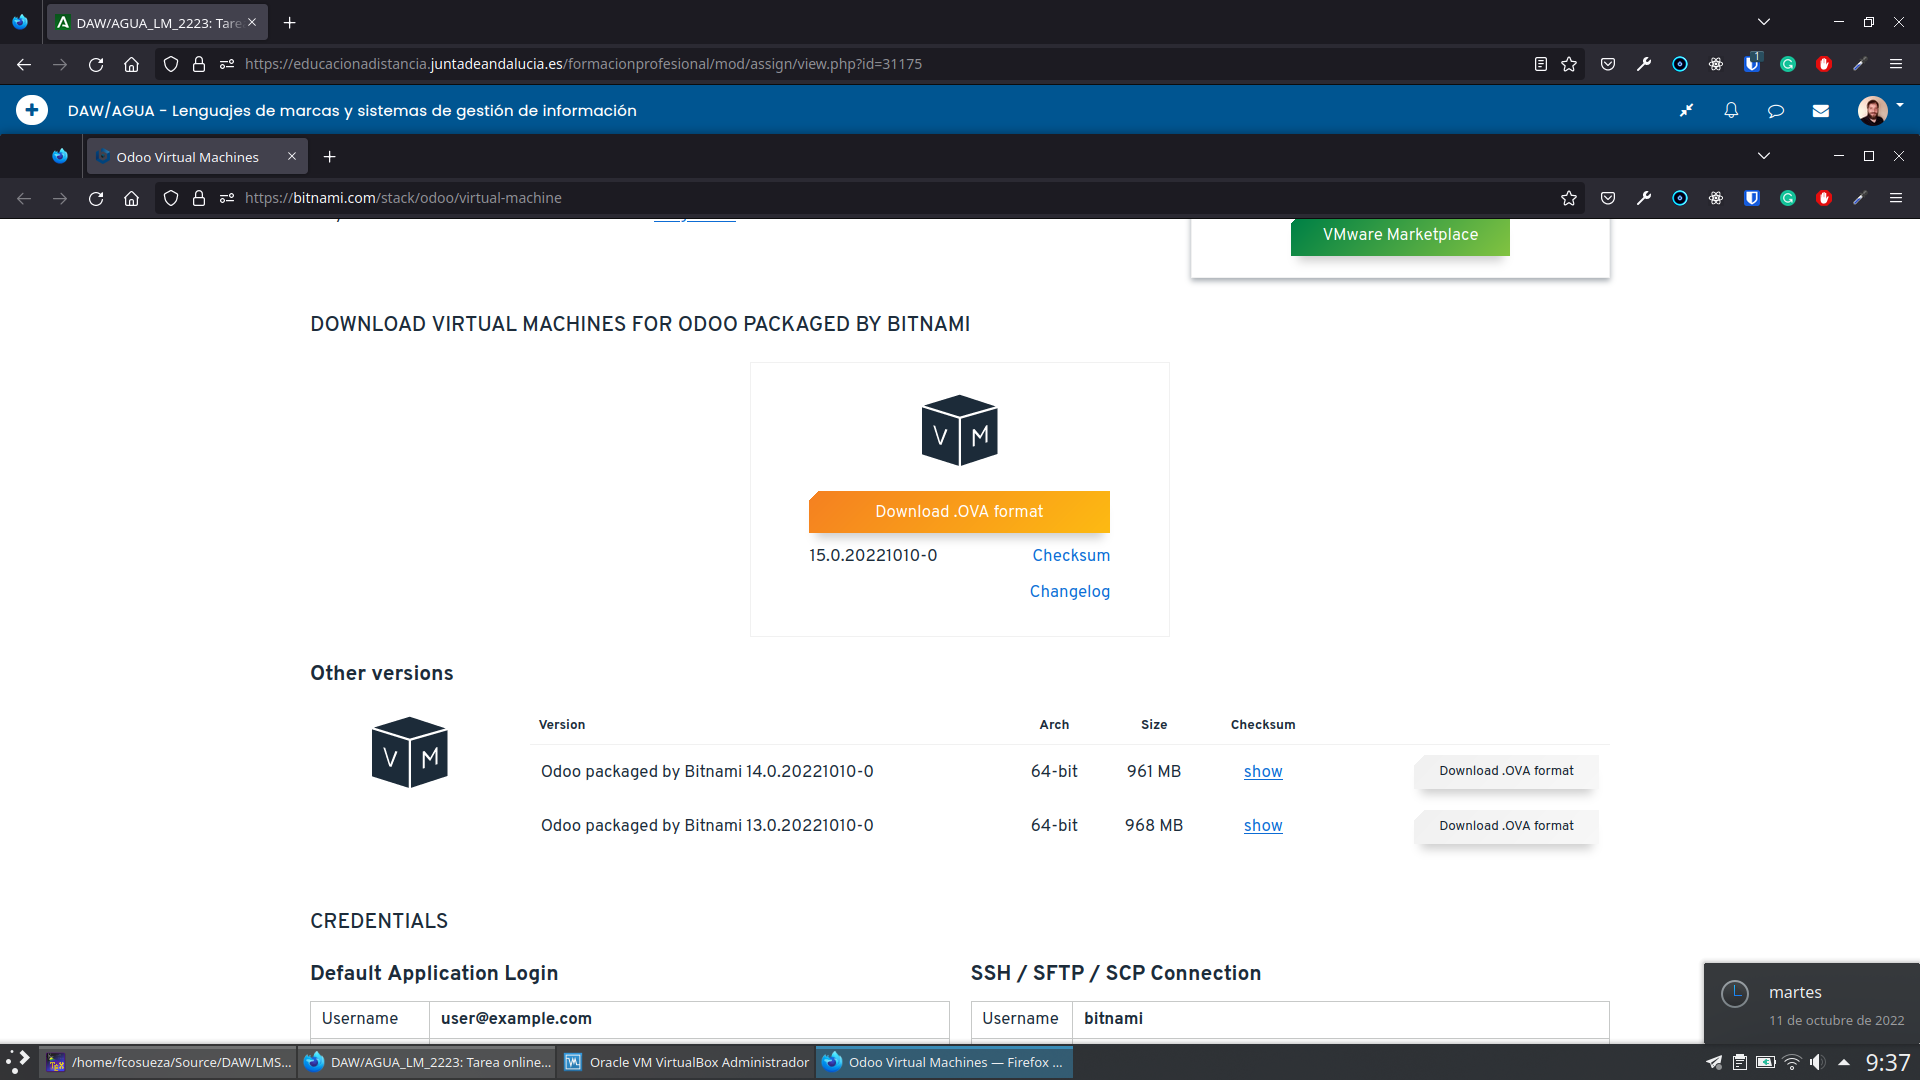
\includegraphics[scale=0.25]{descarga-odoo.png}
    \caption{Página de Bitnami con la imagen de Odoo}
\end{figure}


\subsection{Instalación de la imagen en VirtualBox}
Una vez que tengamos la imagen descargada, tendremos que cargarla en VirtualBox. Para ello, abrimos la aplicaciones y pulsamos el botón importar.

\begin{figure}[ht]
    \centering
    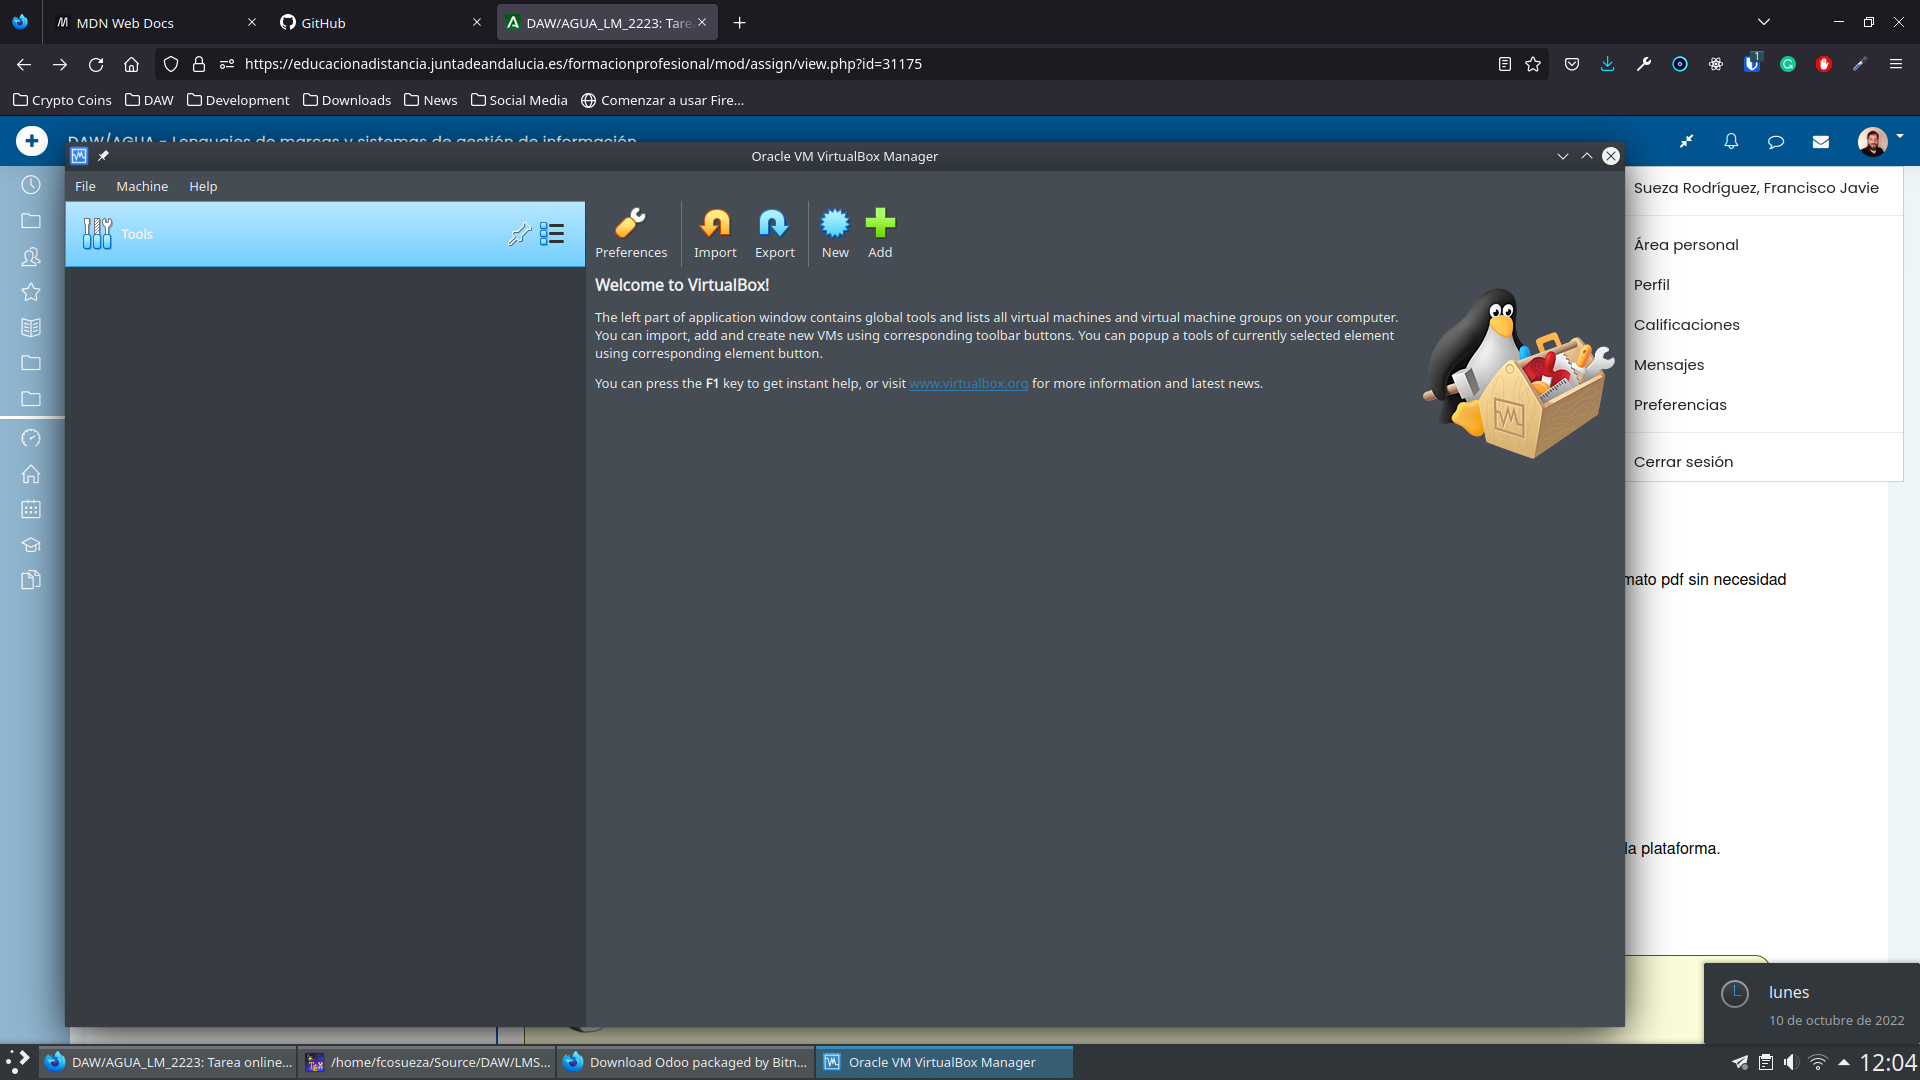
\includegraphics[scale=0.25]{vb-import.png}
    \caption{Pantalla principal de VB}
\end{figure}

A continuación nos saldrá una pantalla donde deberemos seleccionar la imagen que nos hemos descargado y pulsar en siguiente. Una vez seleccionada la imagen, nos mostrará información sobre está, como el tipo de SO, la RAM que utilizará, etc.. Para continuar, deberemos \textbf{pulsar en Importar} de nuevo y la imagen se empezará a cargar en VirtualBox.

Una vez cargada la imagen, ya esta lista para su uso. En la izquierda, tendremos una lista con todas las maquinas virtuales disponibles, en nuestro caso, solo aparece la de Odoo. A la derecha se nos muestra información sobre la máquina virtual seleccionada. Para iniciar la imagen, pulsamos en \textbf{Iniciar}, y comenzará la ejecución de la imagen que hemos descargado.

\begin{figure}[ht]
    \centering
    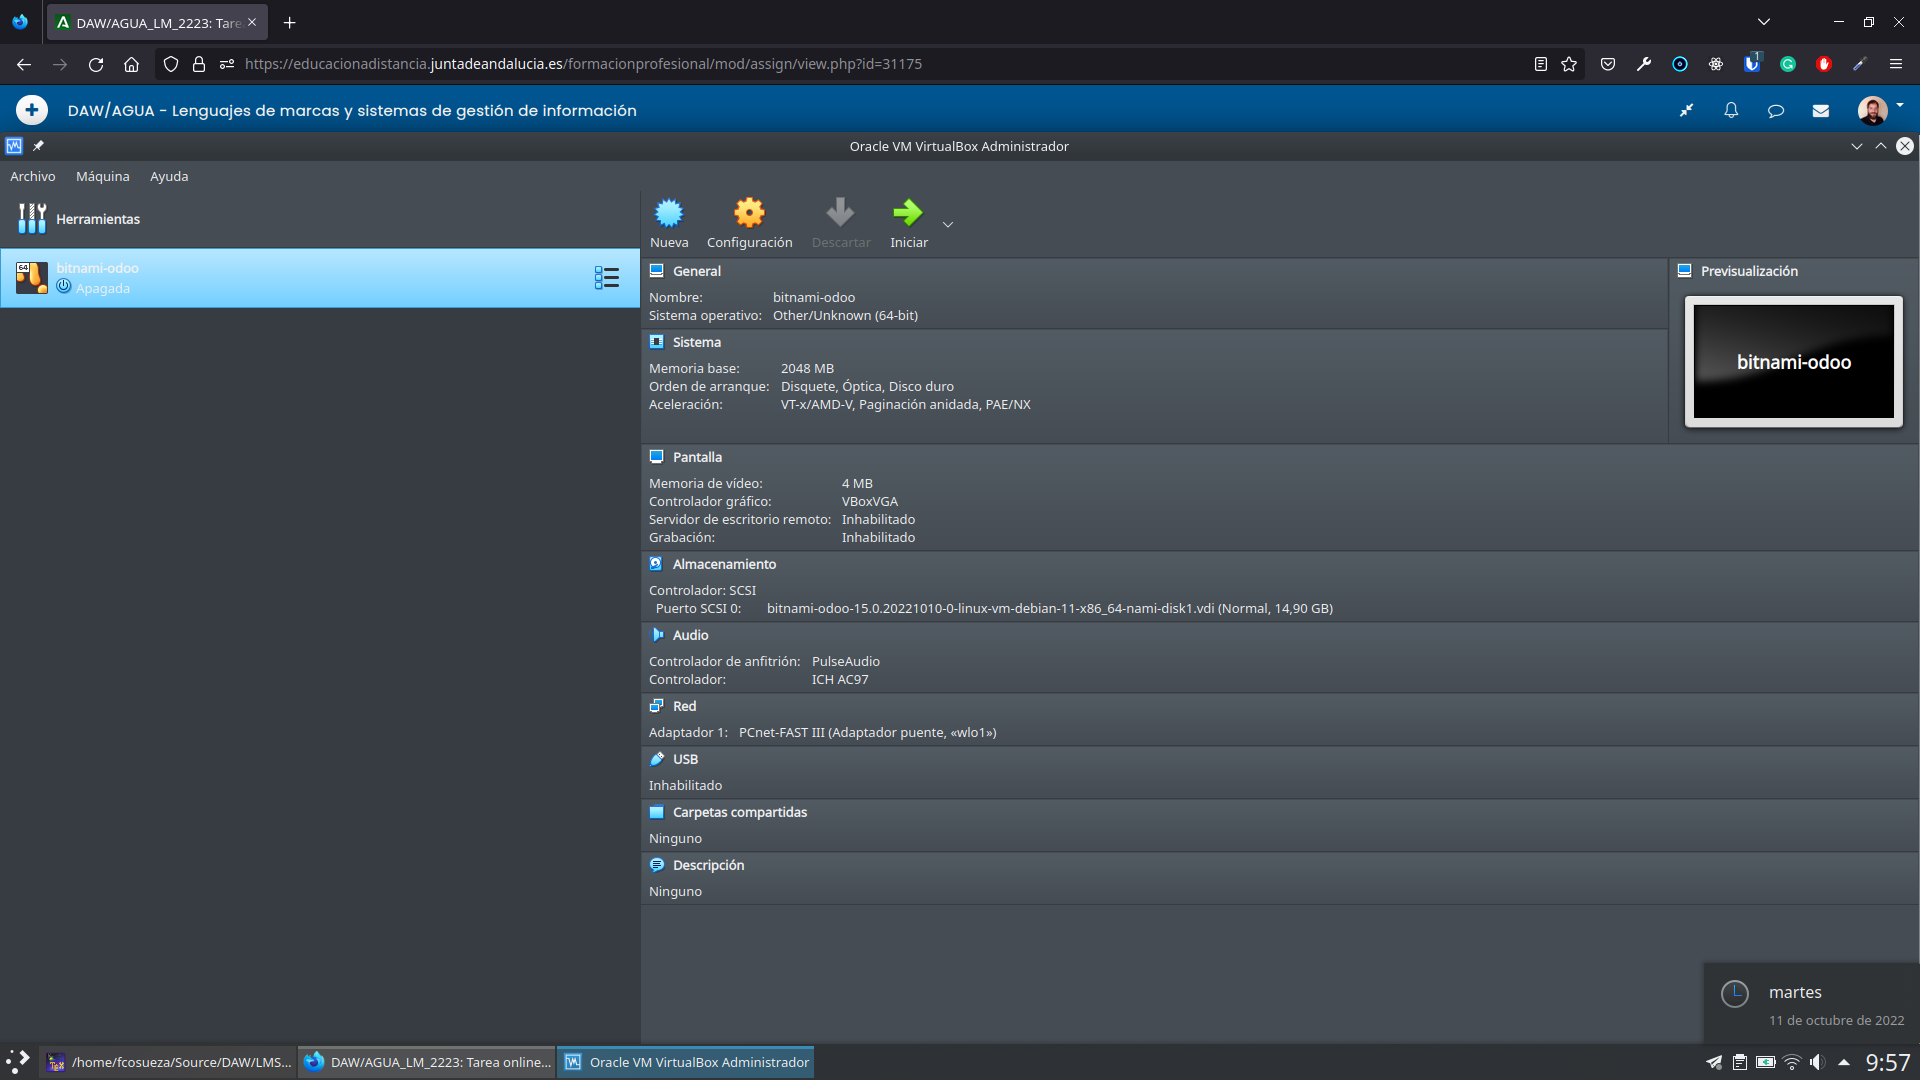
\includegraphics[scale=0.25]{vb-image-info.png}
    \caption{Información de imagen en Virtual Box}
\end{figure}


\subsection{Accediendo a Odoo}
Cuando hayamos iniciado la imagen de Odoo, nos aparecerá una terminal con información muy importante. Por un lado, nos mostrará la \textbf{dirección del servidor} de Odoo, que nos servirá para acceder a la aplicación desde un navegador. Por otro lado, nos mostrará los credenciales por defecto, \textbf{usuario} y \textbf{contraseña}, que nos servirán para hacer login por primera vez.

\begin{figure}[ht]
    \centering
    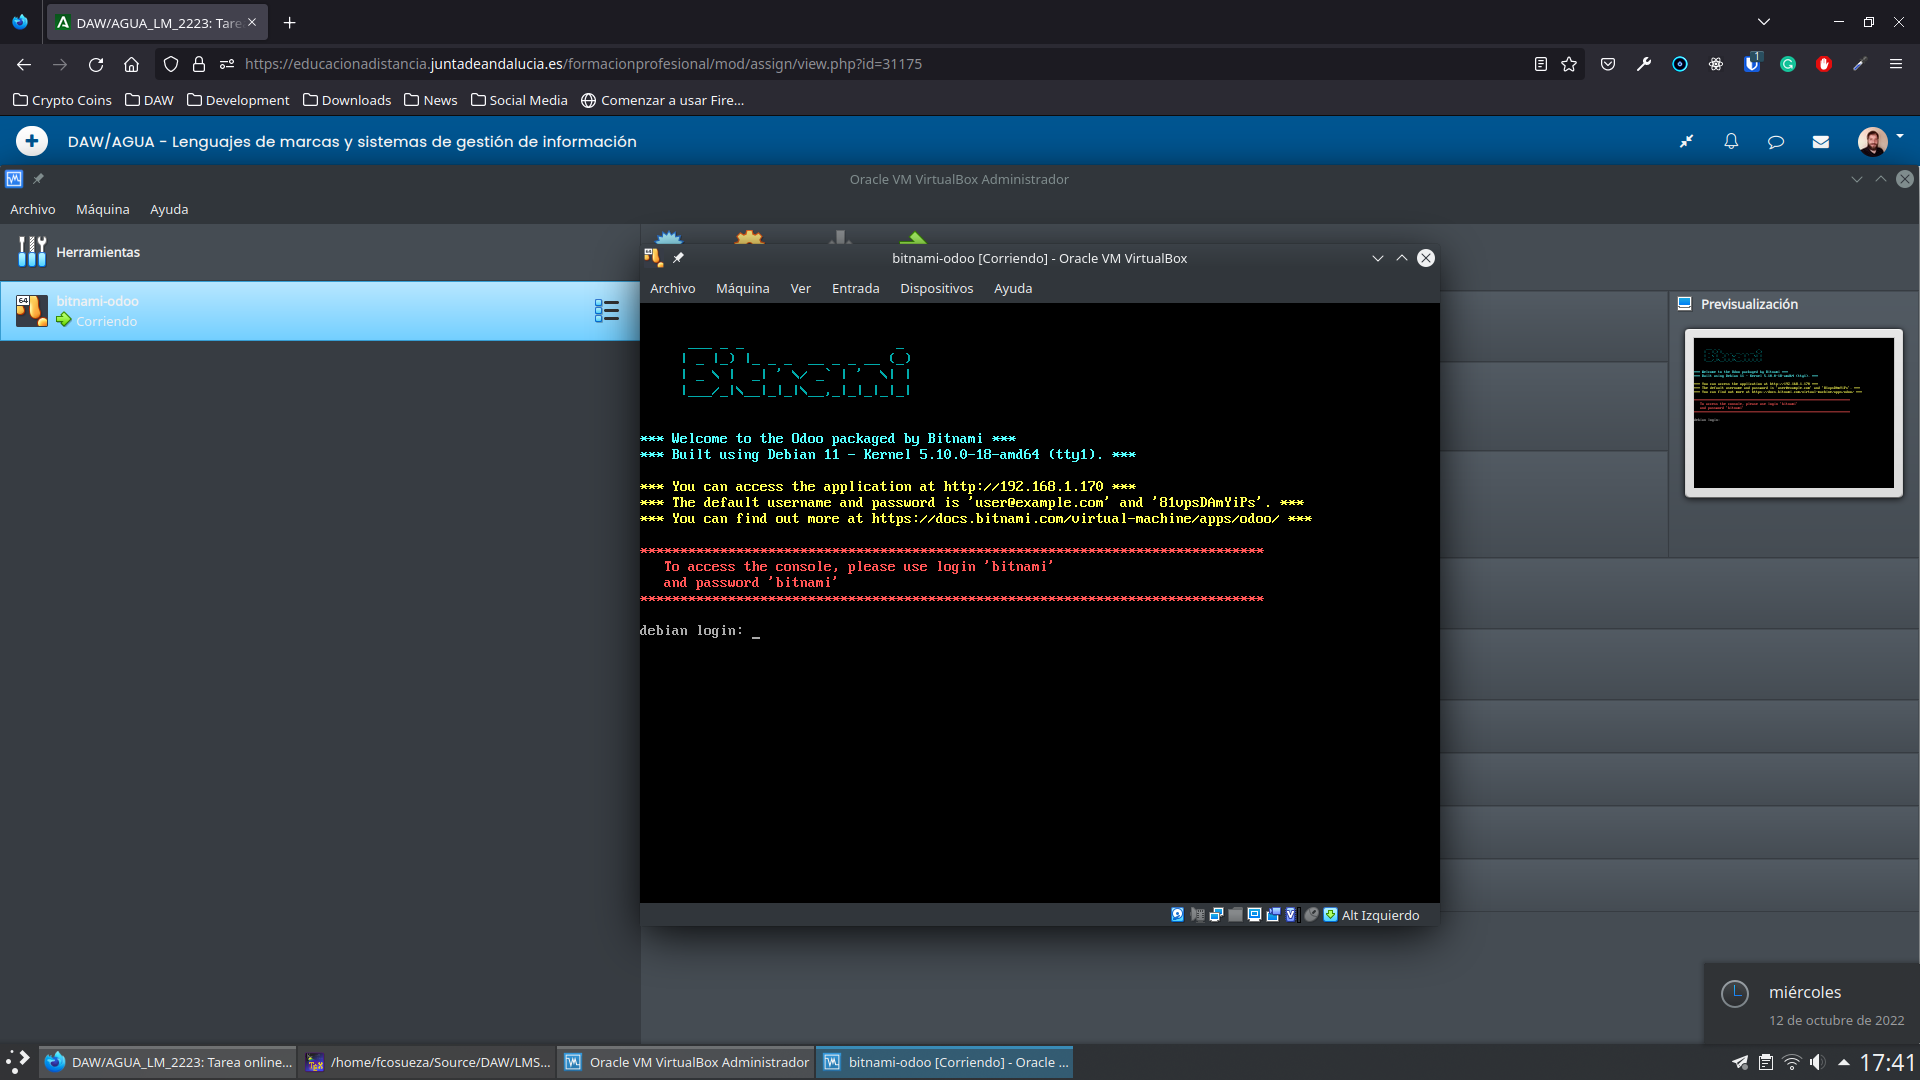
\includegraphics[scale=0.25]{odoo-image-run.png}
    \caption{Terminal inicial de la imagen de Odoo}
\end{figure}

En nuestro caso, la dirección del servidor es \textbf{\textit{http://192.168.1.170}}, mientras que el usuario de acceso a Odoo es \textbf{\textit{user@example.com}} y la contraseña \textbf{\textit{81vpsDAmYiPs}}.

Con estos datos, abrimos un navegador, no importa cual sea, e introducimos la dirección del servidor en la barra de direcciones. Lo que nos mostrará la pantalla inicial de inicio de sesión de Odoo. A continuación introducimos el usuario y la contraseña proporcionados y pulsamos en \textbf{Log in}.


\begin{figure}[ht]
    \centering
    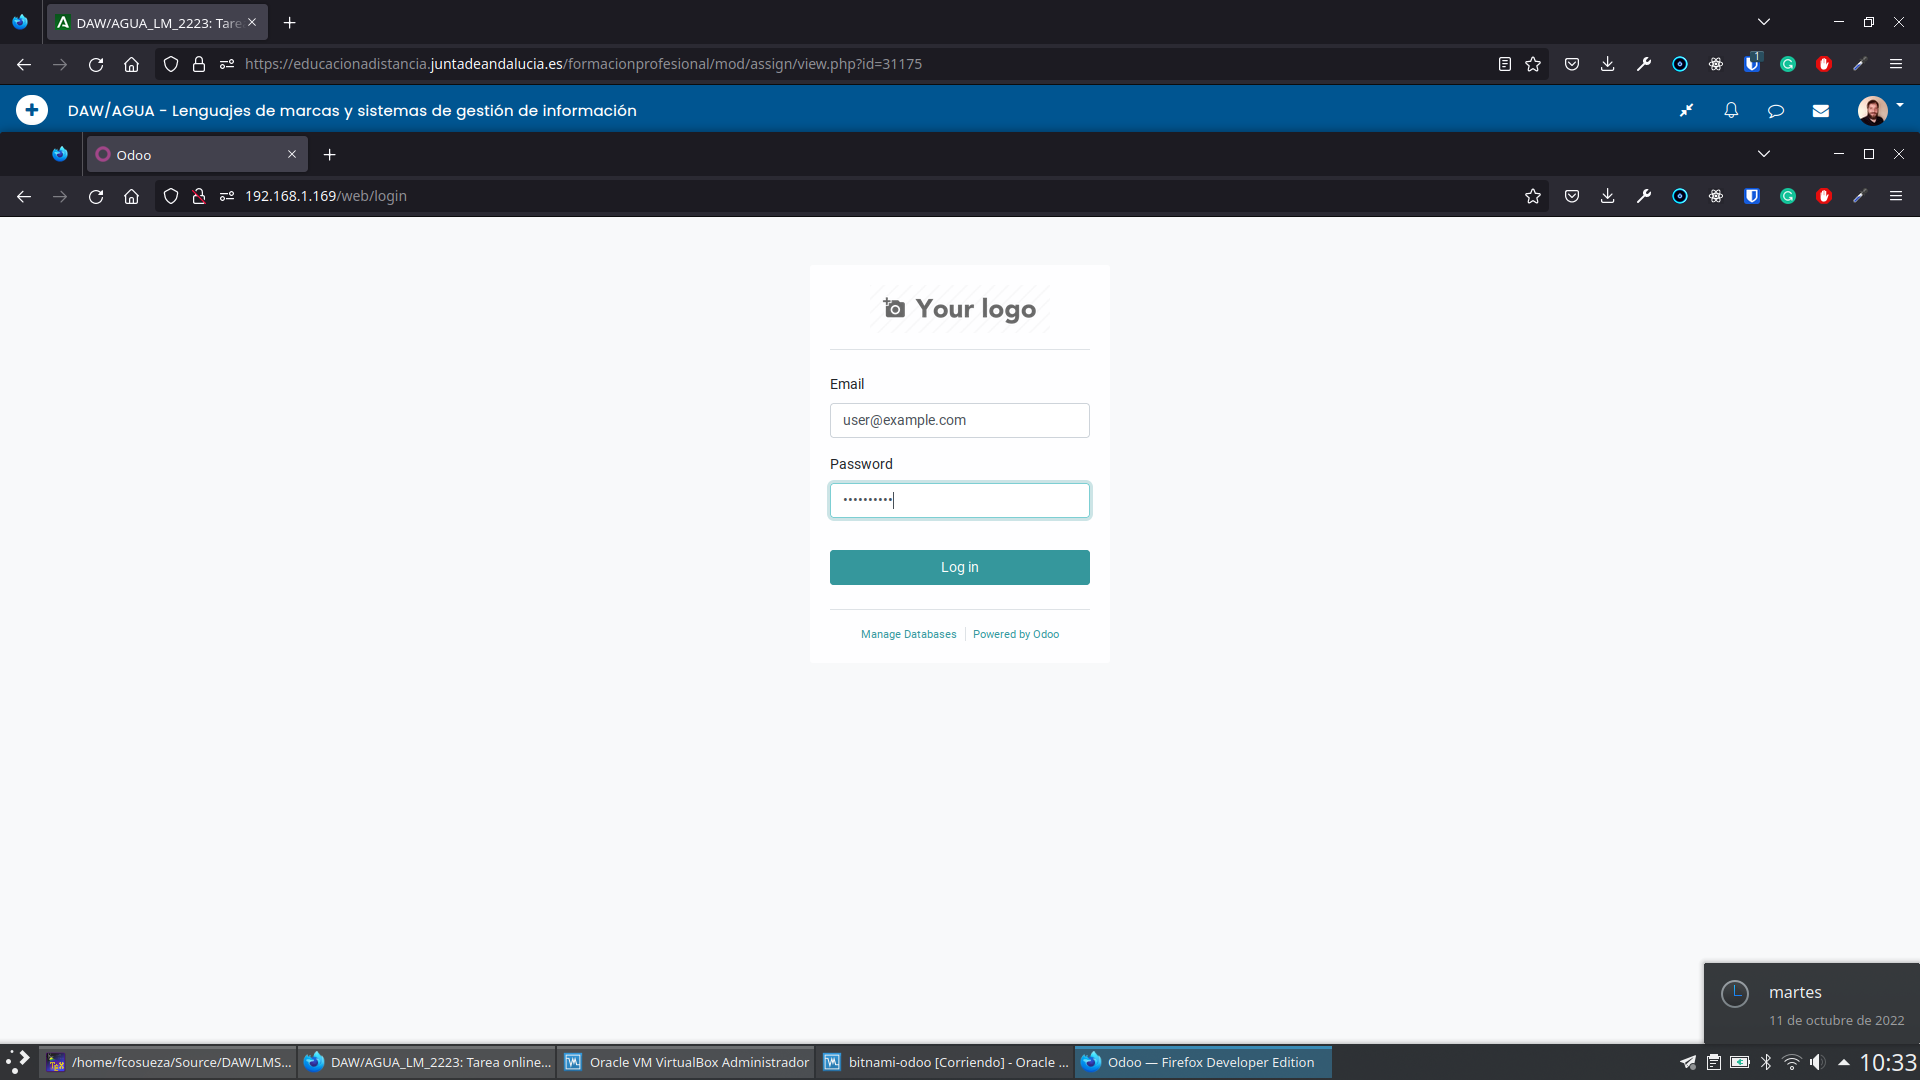
\includegraphics[scale=0.25]{login-odoo.png}
    \caption{Pantalla de inicio de sesión de Odoo}
\end{figure}

\subsection{Cambio de Contraseña e Idioma}
Después de haber iniciado sesión, nos parecerá la pantalla principal de Odoo. Aquí se nos muestran todos los\textbf{ módulos disponibles} para instalar. A la izquierda, podemos \textbf{seleccionar una categoría} y que nos muestre solo los módulos que pertenecen a dicha categoría. Como podemos ver arriba a la derecha, ya se ha creado un \textbf{usuario por defecto}, llamado \textbf{Administrator} y arriba a la izquierda tenemos un \textbf{menú desplegable}.

\begin{figure}[ht]
    \centering
    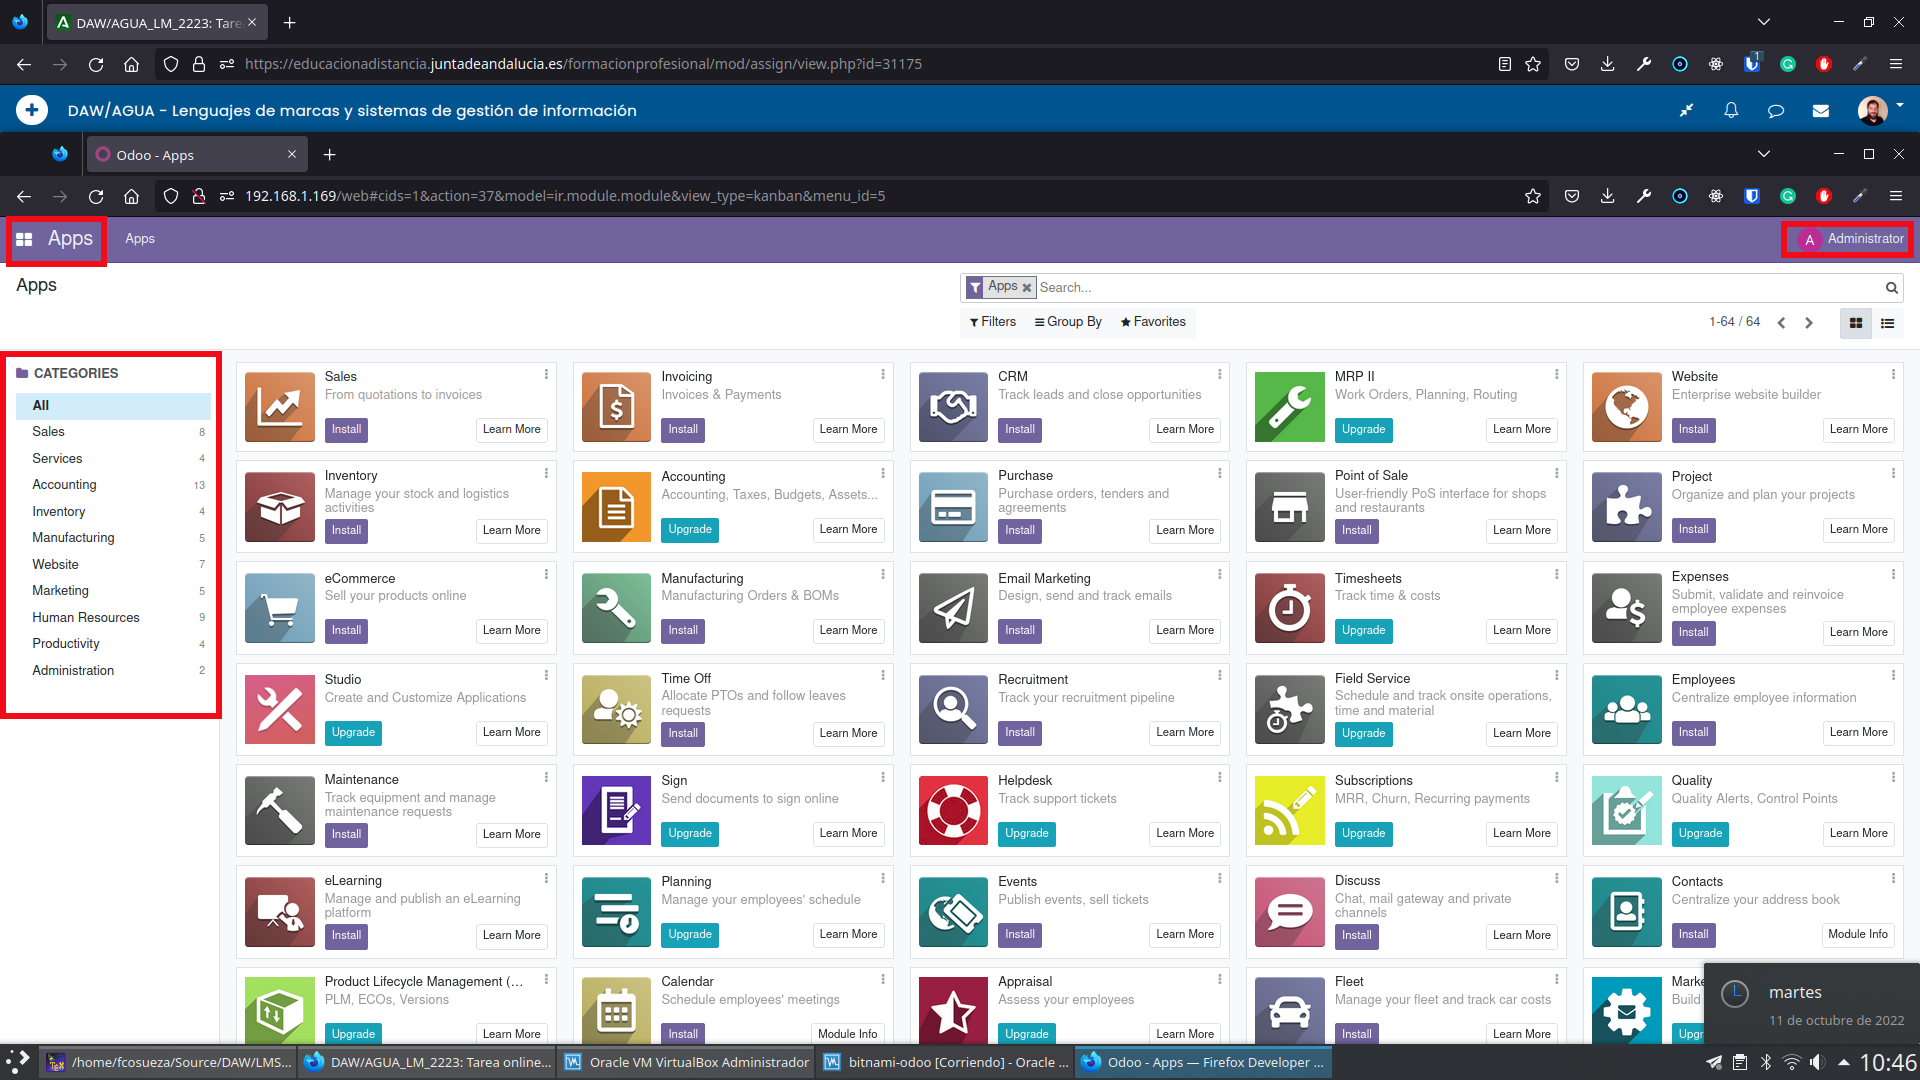
\includegraphics[scale=0.25]{main-odoo.png}
    \caption{Pantalla principal de Odoo}
\end{figure}

Lo primero que deberíamos hacer, es cambiar la \textbf{contraseña de administrador} por la que nosotros queramos. Es conveniente, como en cualquier otra aplicación, utilizar una contraseña fuerte, que sea larga y que alterne números, letra en minúscula y mayúscula, etc..

\begin{enumerate}
    \item Abrimos el menú desplegable, que se encuentra arriba a la derecha, y pulsamos en la opción \textbf{Settings}, que nos abrirá por defecto la pantalla \textbf{Users}.

    \begin{figure}[ht]
        \centering
        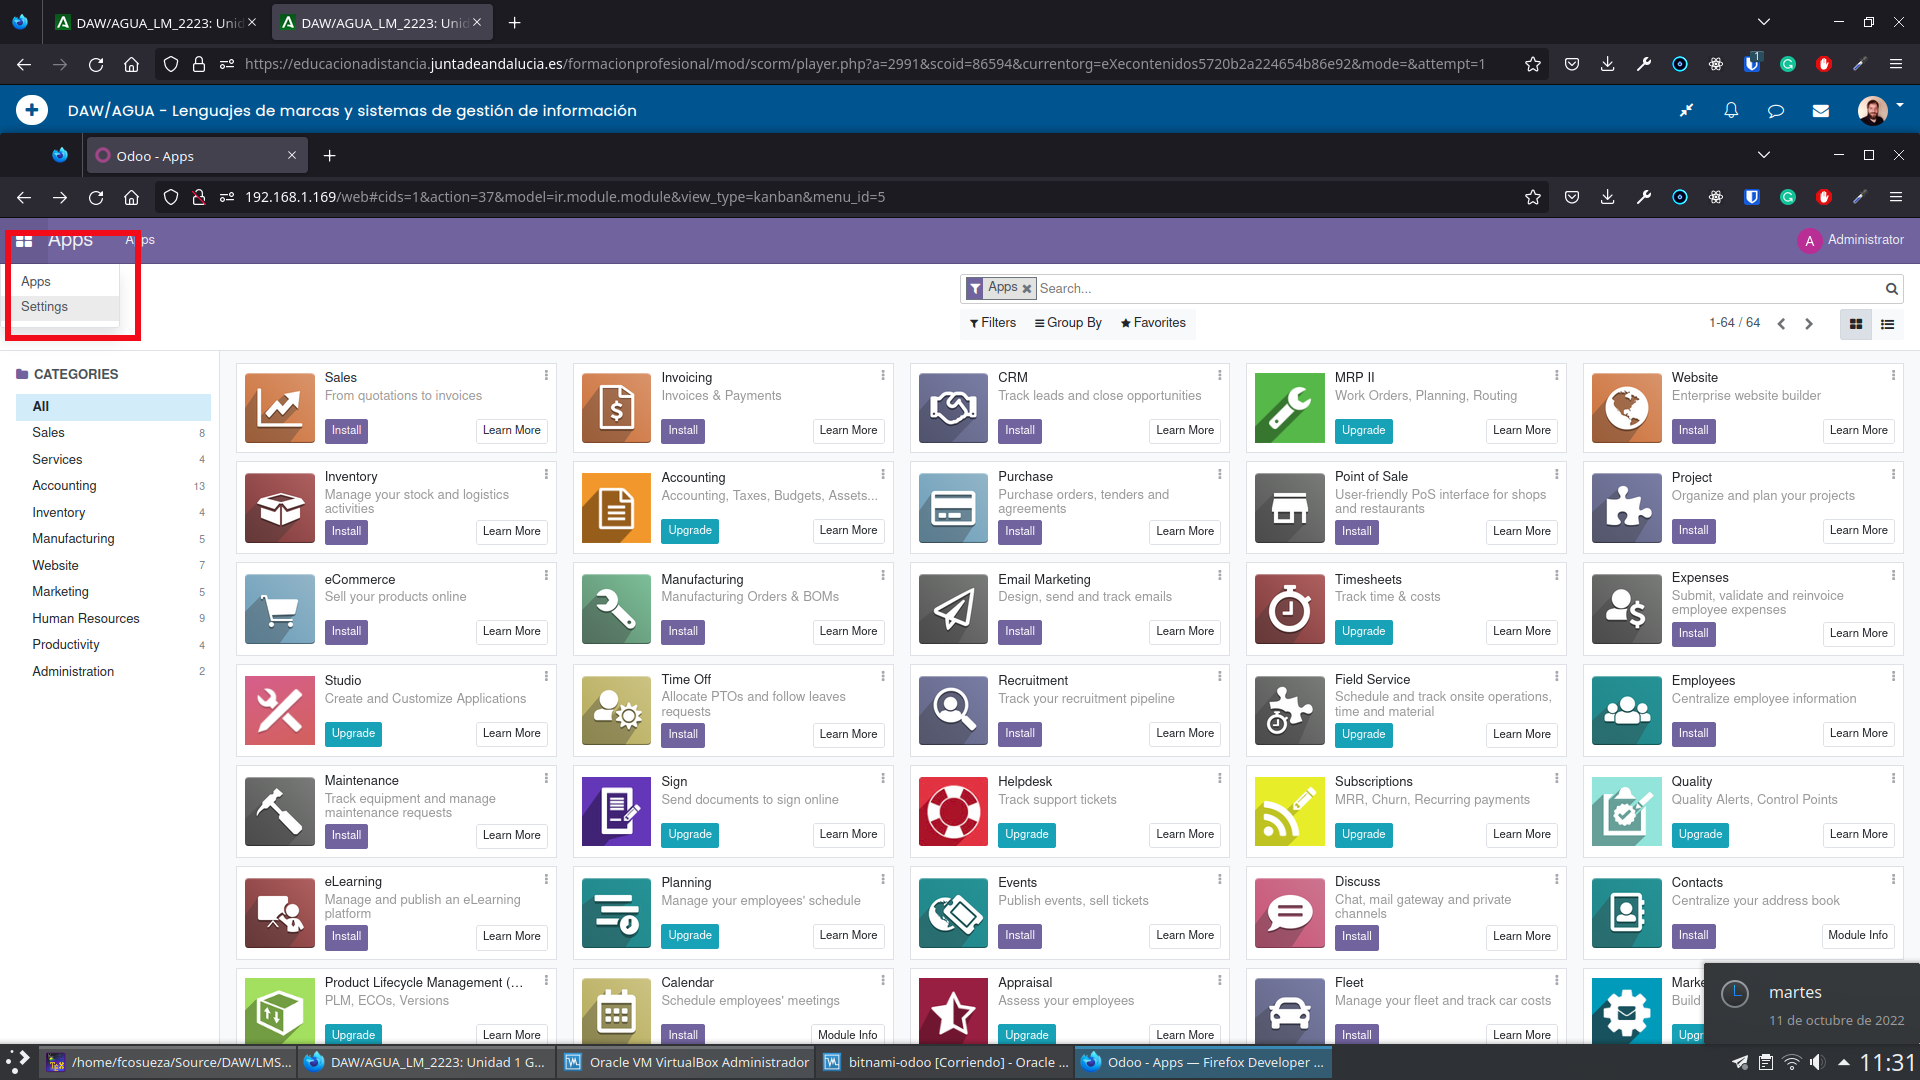
\includegraphics[scale=0.25]{change-pass-01.png}
        \caption{Opción Setting del menú desplegable}
    \end{figure}

    \item En la siguiente pantalla, se nos mostrará la lista de usuarios, en nuestra caso solo tenemos al usuario \textbf{Admnistrator}, seleccionamos este usuario.

    \begin{figure}[ht]
        \centering
        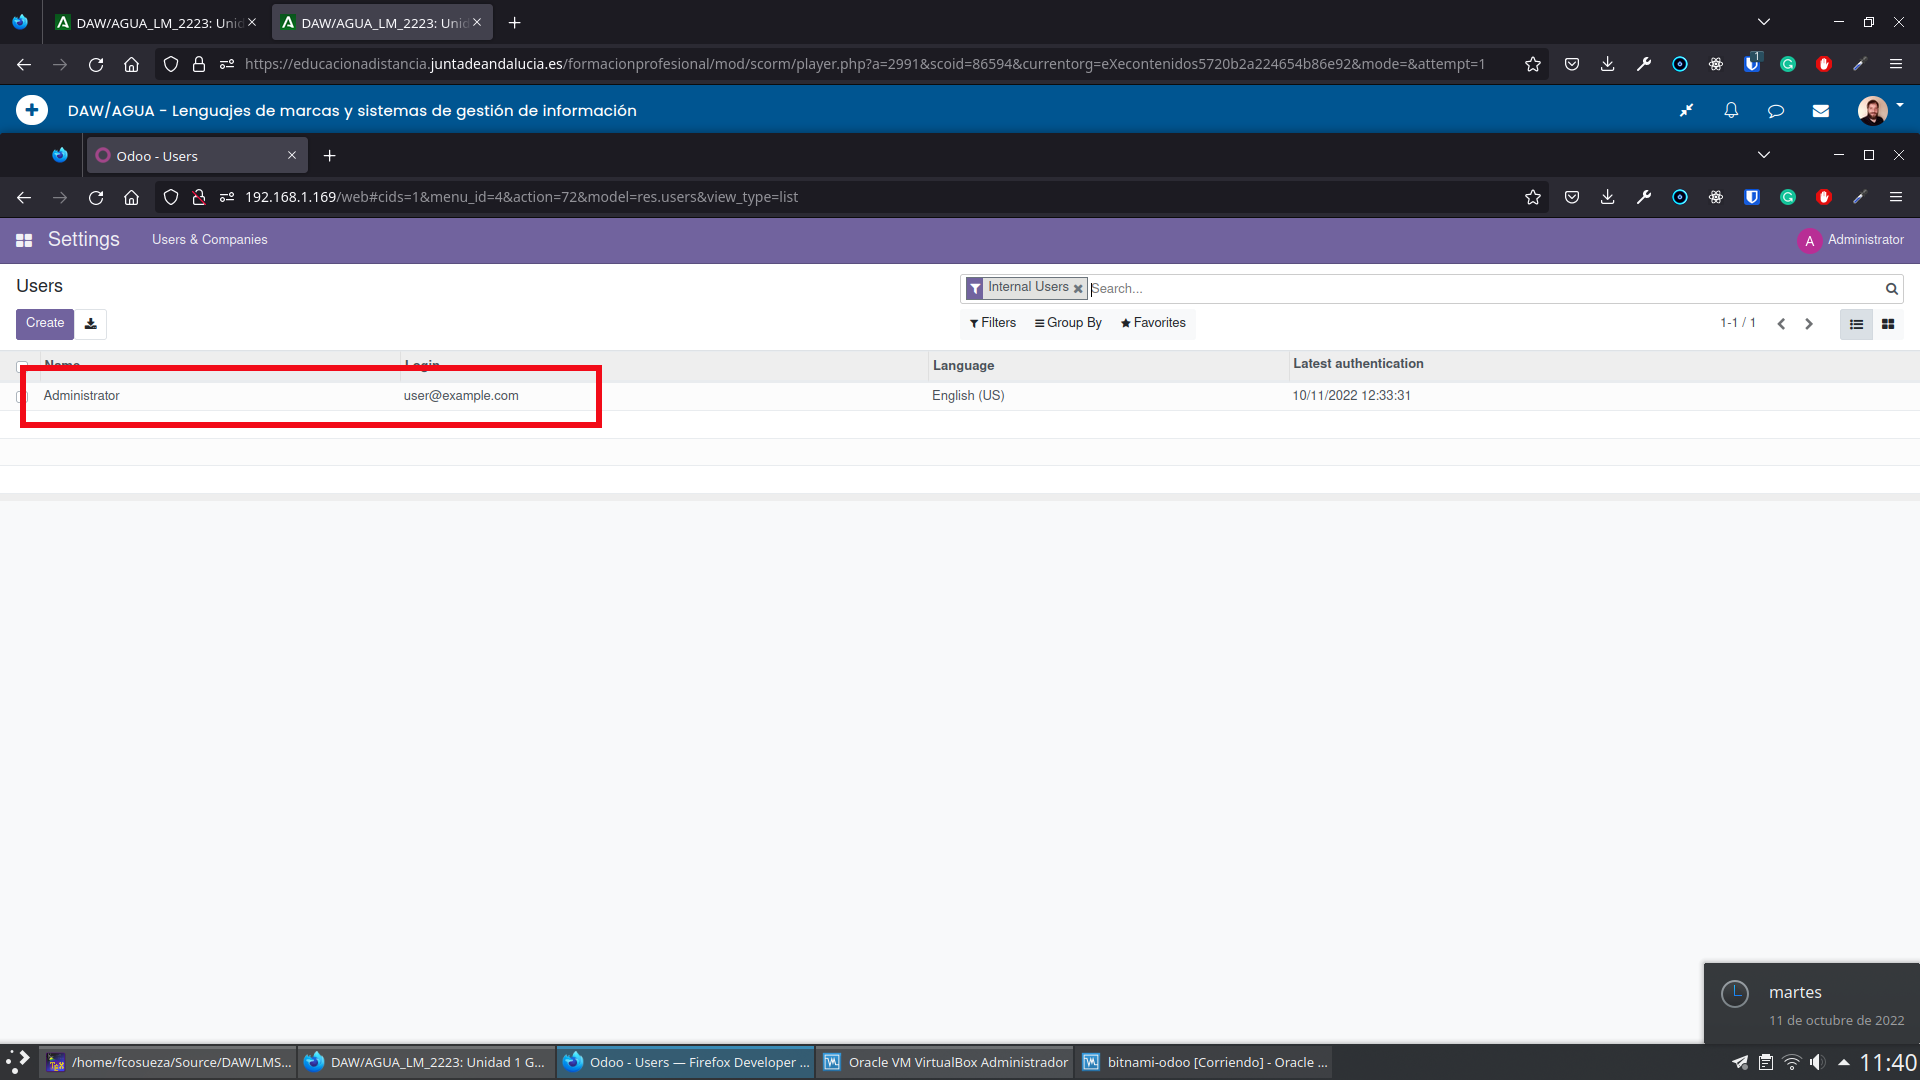
\includegraphics[scale=0.25]{change-pass-02.png}
        \caption{Pantalla de gestión de usuarios de Odoo}
        \label{fig:user}
    \end{figure}

    \item Una vez hayamos seleccionado el usuario nos mostrará una pagina con un ficha con información del usuario, como su correo, el nombre, una foto, en caso de que la tenga, y en la parte inferior los derechos de acceso (Access Rights), las preferencias (Preferences) y la configuración de seguridad de la cuenta (Account Security).

    Como a nosotros solo nos interesa, cambiar la contraseña, vamos a desplegar el \textbf{menú Action}, que se encuentra en la parte superior, y seleccionar la opción \textbf{Change Password}.

    \vspace{8ex}

    \begin{figure}[ht]
        \centering
        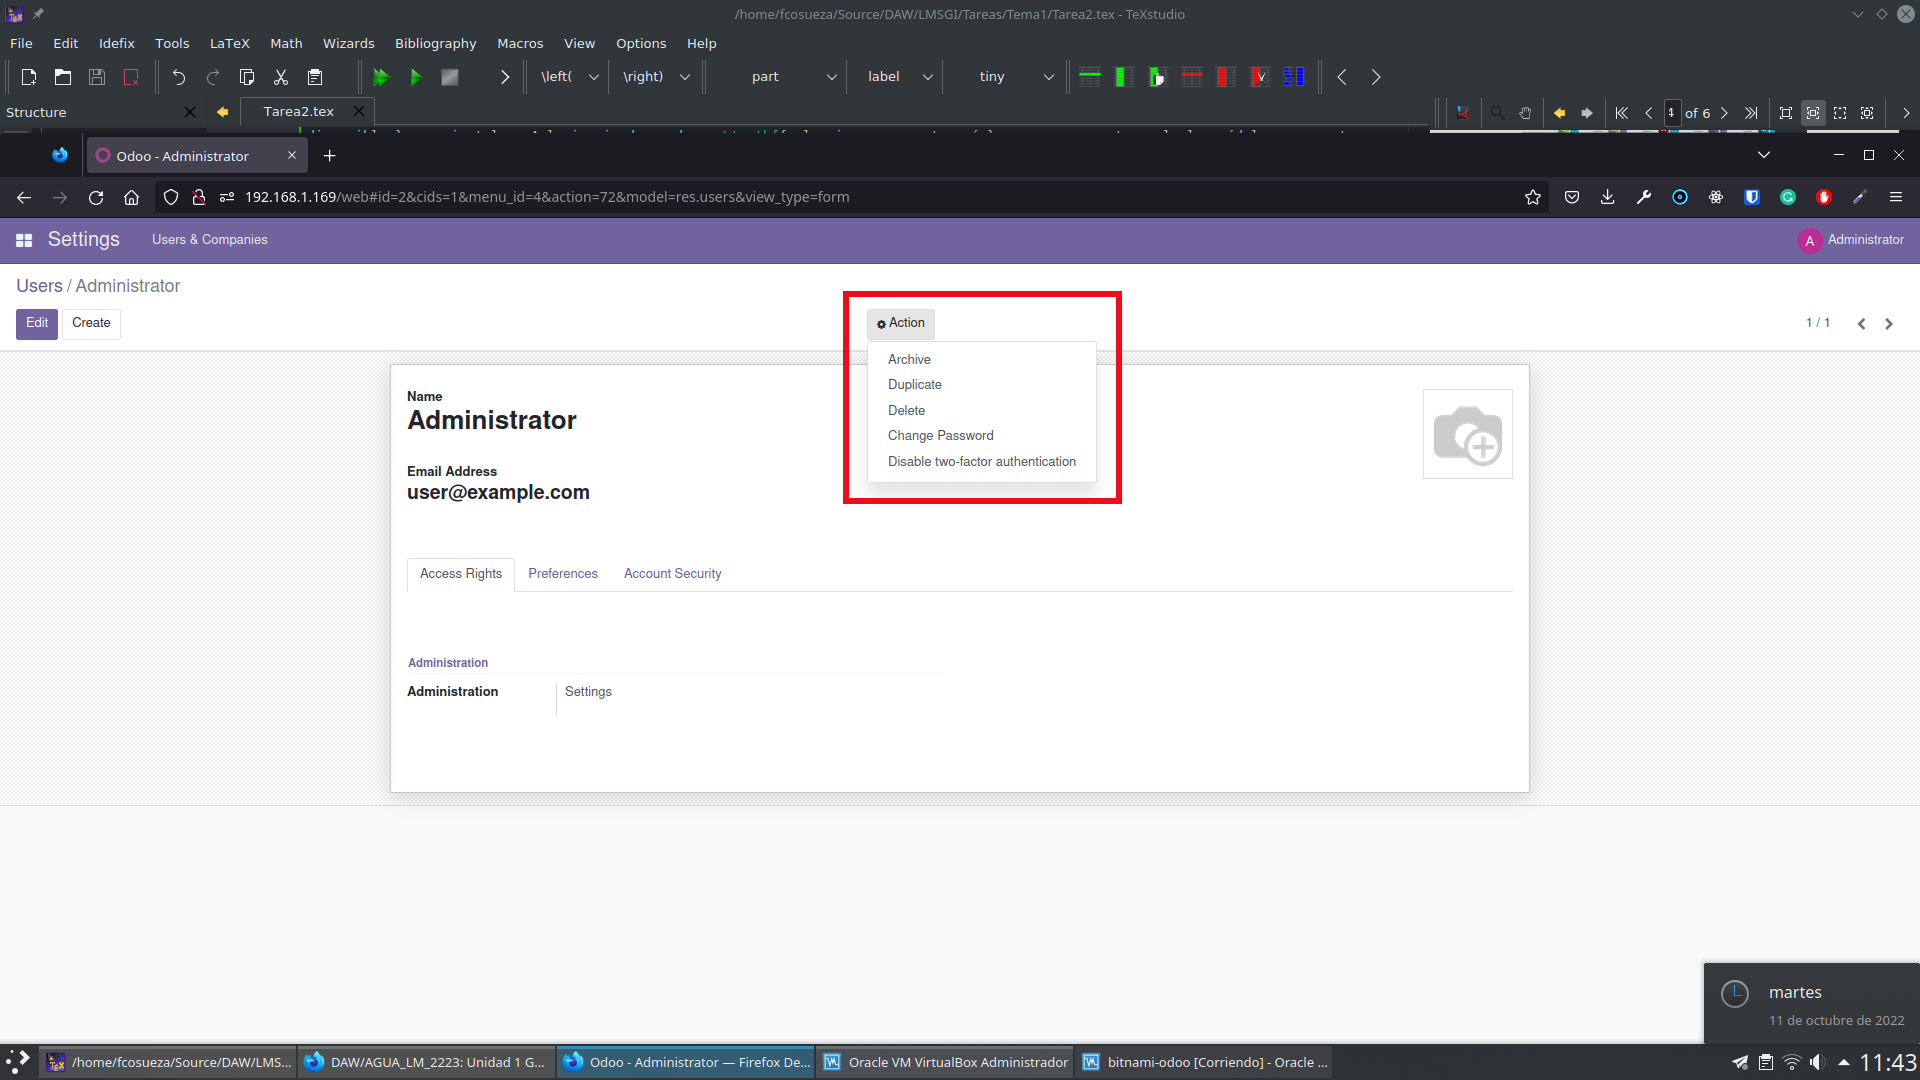
\includegraphics[scale=0.25]{change-pass-03.png}
        \caption{Pantalla con ficha de usuario}
        \label{fig:card}
    \end{figure}

    \item A continuación aparecerá una pantalla donde se nos mostrará el usuario y al lado un una entrada de formulario para introducir la nueva contraseña. La introducimos, pulsamos el botón \textbf{Change Password} y se habrá completado el proceso. Tras el cambio, no redirigirá a la pantalla de Log In.

    \begin{figure}[ht]
        \centering
        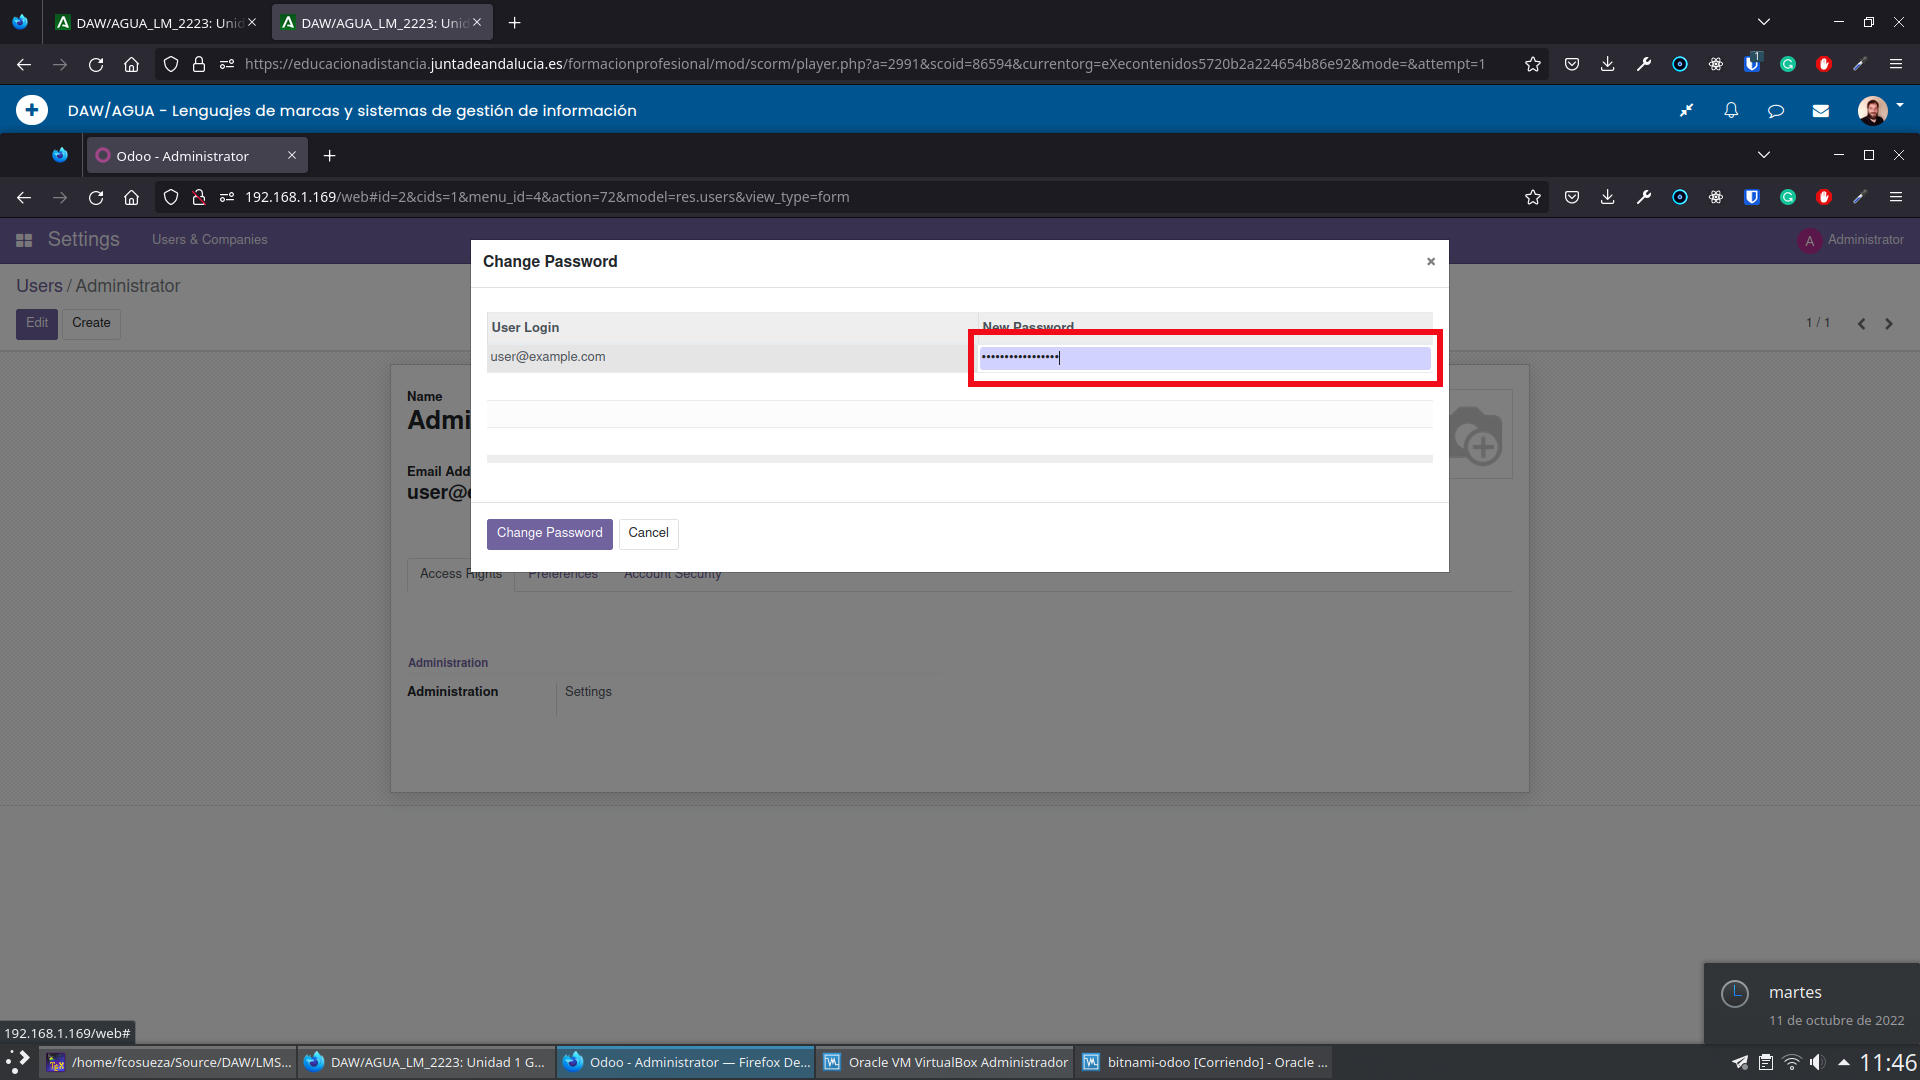
\includegraphics[scale=0.25]{change-pass-04.png}
        \caption{Pantalla de cambio de contraseña}
    \end{figure}
\end{enumerate}

Una vez cambiada la contraseña, vamos a \textbf{cambiar el idioma} y ponerlo en español. Para ello, vamos a seguir los siguientes pasos.

\begin{enumerate}
    \item Desde la pagina donde nos aparece la ficha de usuario, como en la Figura \ref{fig:card}, pulsamos en el botón \textbf{Edit} que se encuentra en la parte superior izquierda. Una vez pulsado ahí, pulsamos en la pestaña \textbf{Preferences}, que nos encontramos en el centro debajo del \textbf{email} del usuario.

    \vspace{10ex}

   \begin{figure}[ht]
       \centering
       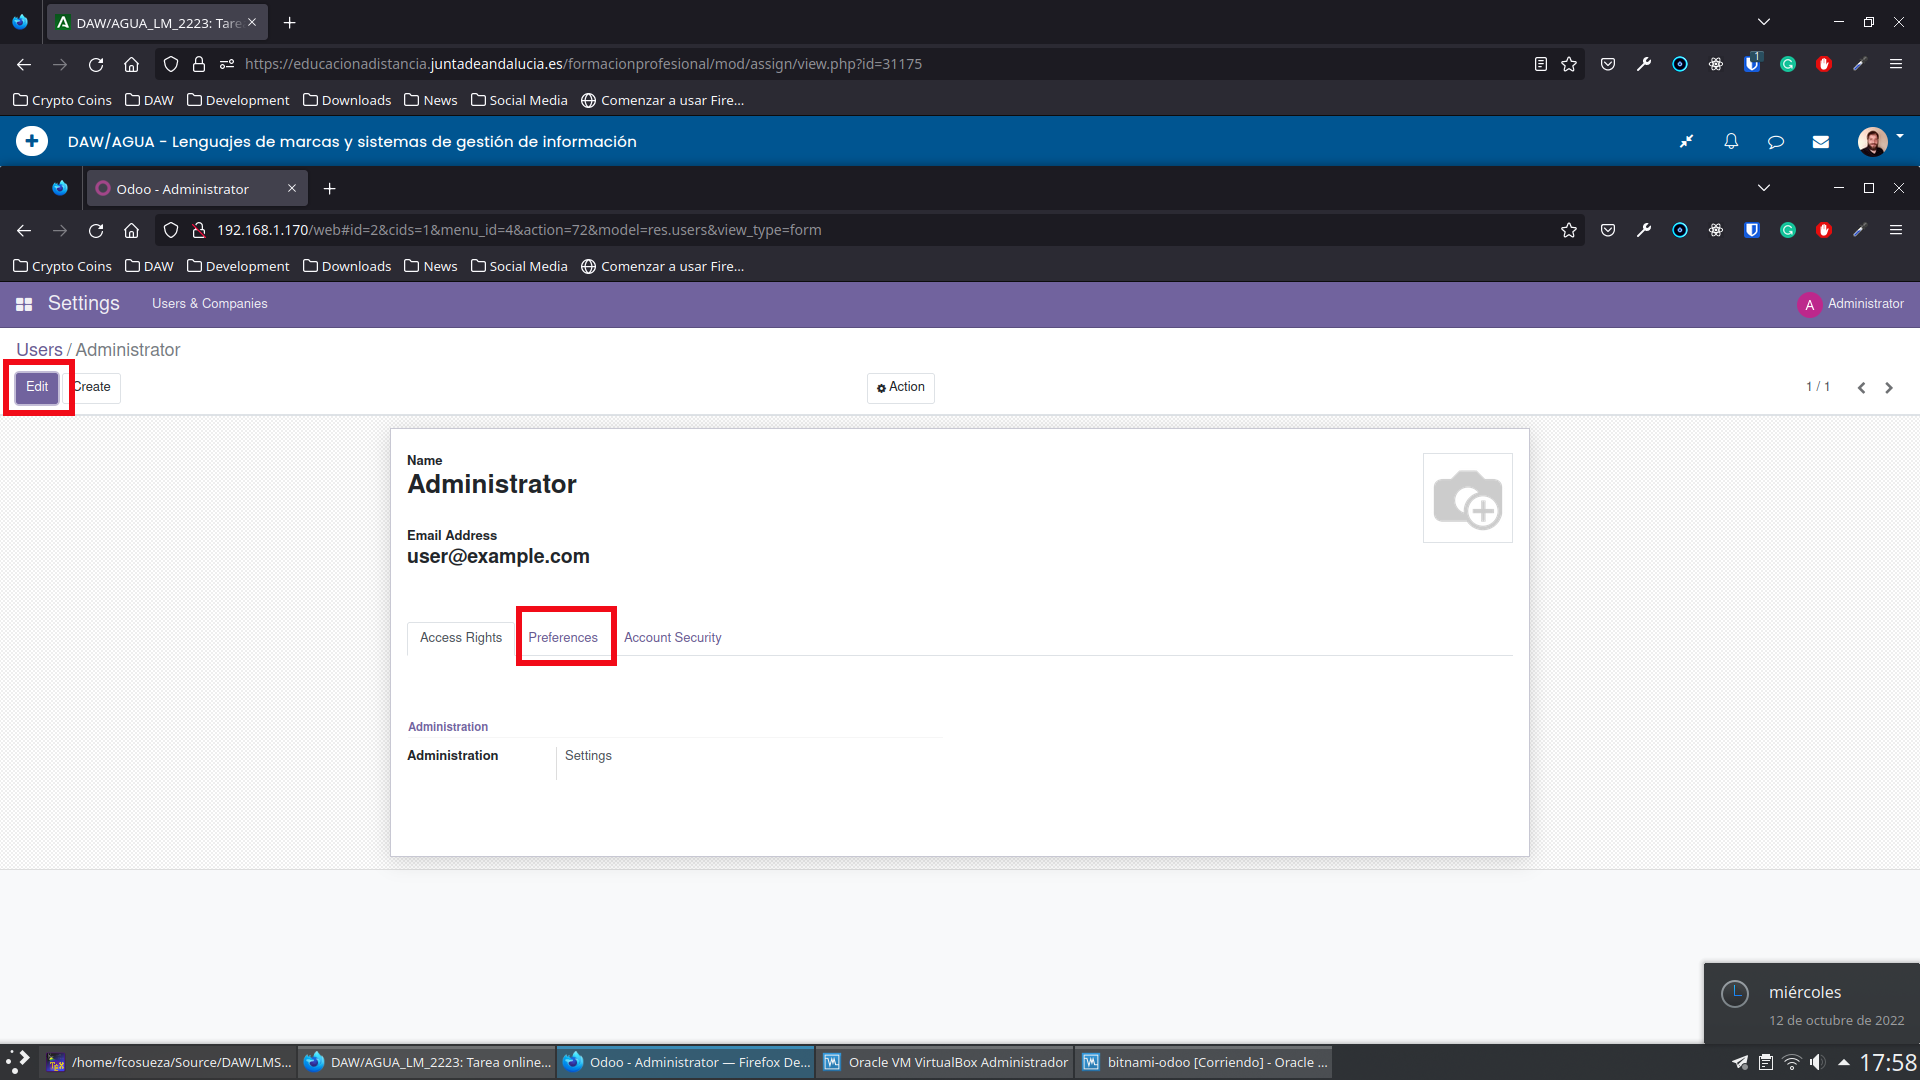
\includegraphics[scale=0.25]{ficha-usuario.png}
       \caption{Ficha de usuario y botón Edit}
   \end{figure}

   \item Dentro de la pestaña \textbf{Preferences}, debemos pulsar en el \textbf{icono} en los aparece a la derecha del menú desplegable de la opción \textbf{Language}.

   \begin{figure}[ht]
       \centering
       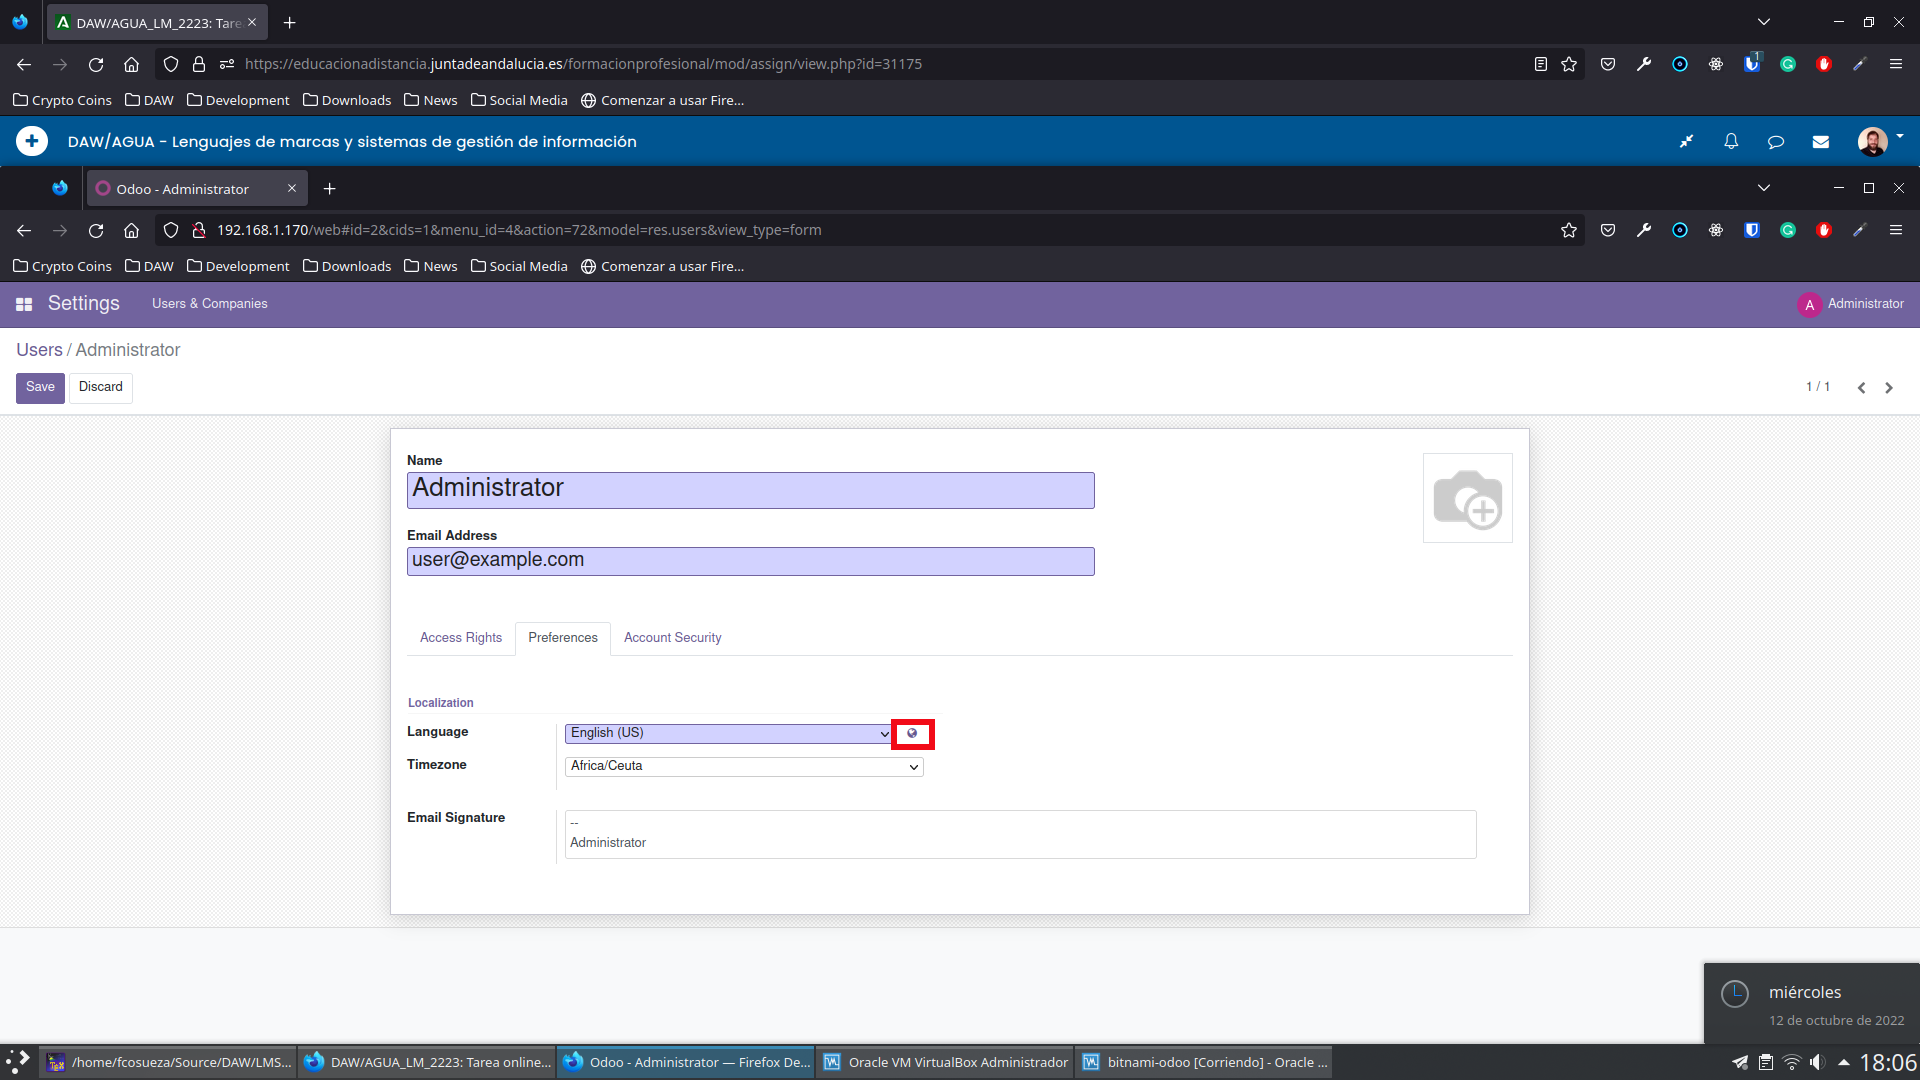
\includegraphics[scale=0.25]{ficha-usuario-preferences.png}
       \caption{Ficha de usuario, pestaña Preferences}
   \end{figure}

   \item Nos saldrá una lista de idiomas, debemos buscar la opción \textbf{Spanish}, marcar la casilla que nos encontraremos a su izquierda y pulsar en \textbf{Activate}, que se encuentra en la misma fila a la derecha. Una vez que hayamos pulsado, se nos abrirá una ventana emergente. Ahí deberemos pulsar en la opción \textbf{Add} y posteriormente en la opción \textbf{Switch to spanish/español \& Close}.

   Una vez hecho esto, ya habremos cambiado el idioma para este usuario. Si queremos cambiarlo para toda la aplicación, el procedimiento es diferente y no se cubre en este documento.

    \vspace{15ex}
   \begin{figure}[ht]
       \centering
       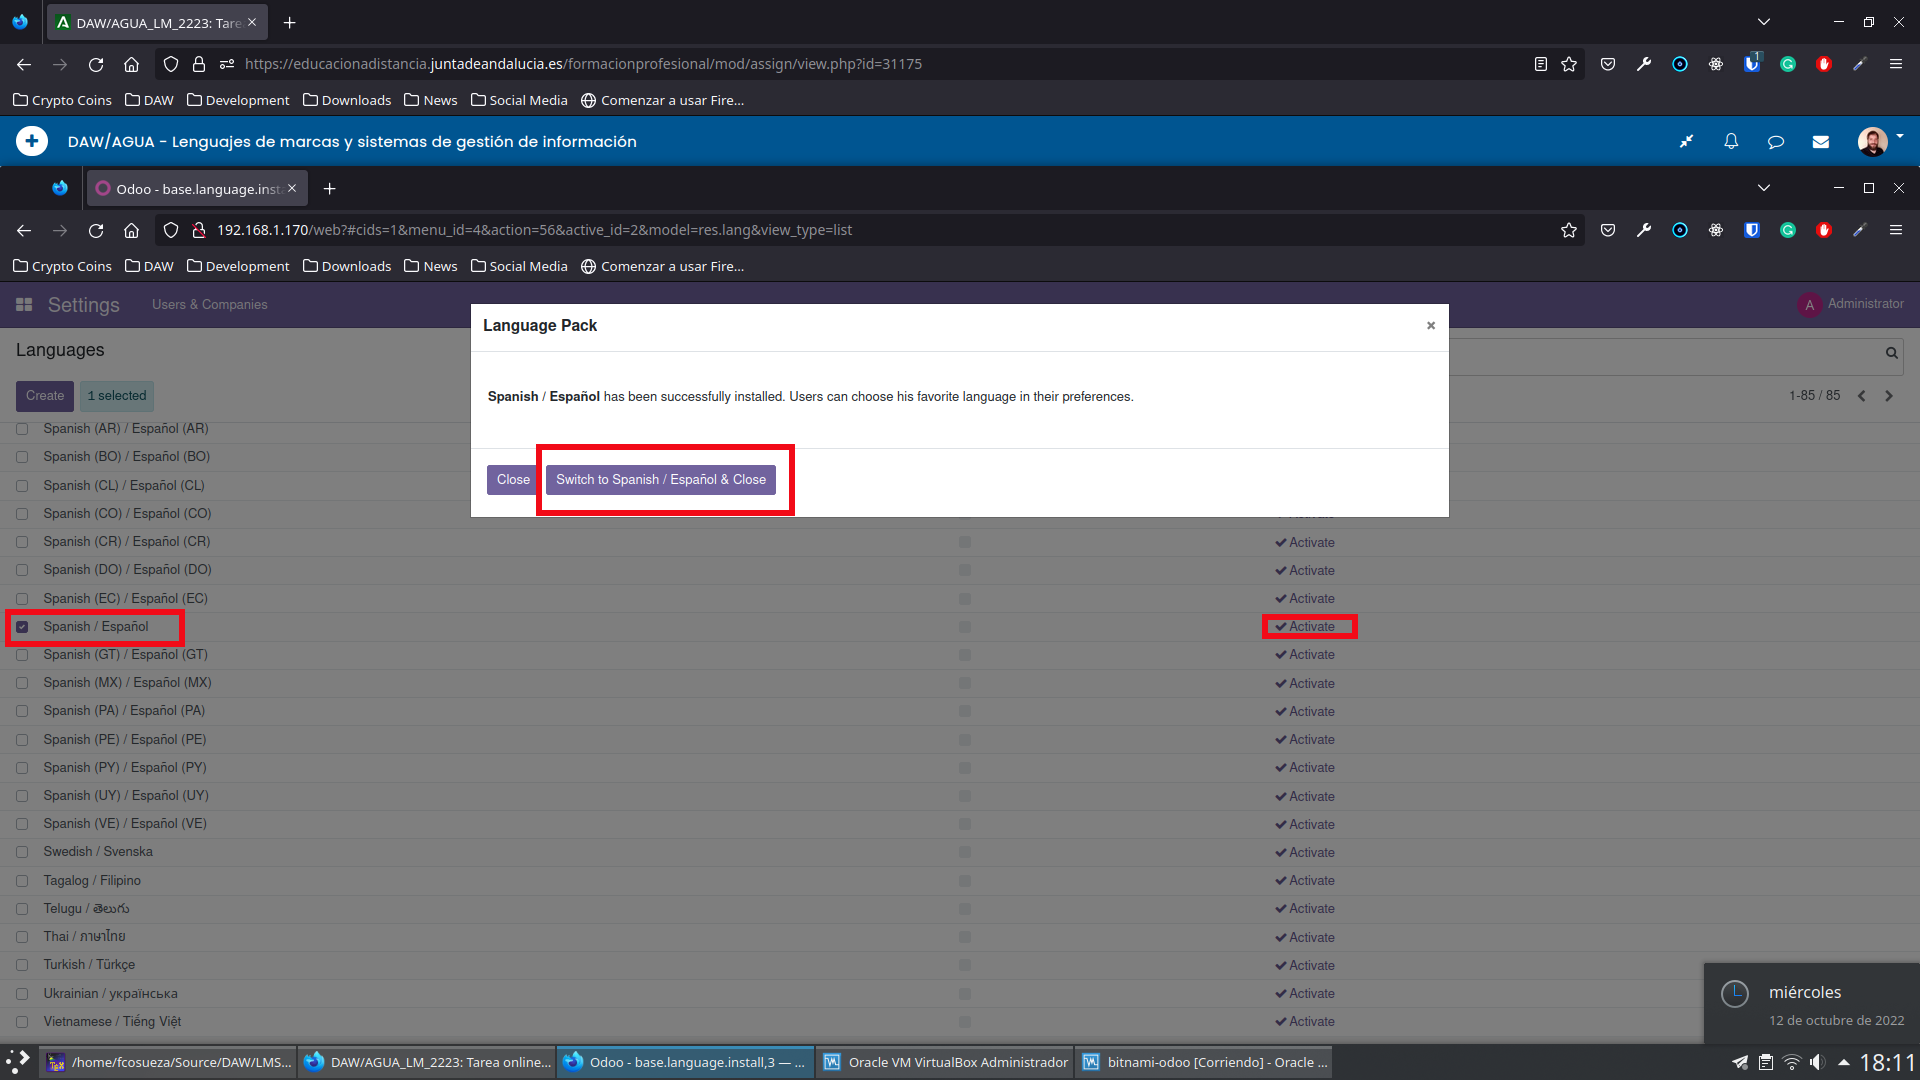
\includegraphics[scale=0.25]{language-switch.png}
       \caption{Cambio de lenguaje a español}
       \label{fig:lang}
   \end{figure}
\end{enumerate}

\section{Datos de la Empresa y Creación Usuarios}

En este punto vamos a añadir los datos de nuestra empresa ficticia \textit{Llegaya S.L}, y posteriormente crearemos dos usuarios.

\subsection{Datos de la Empresa}
Primero vamos ha añadir los datos de nuestra empresa. Para ello, vamos a seguir los siguientes pasos.

\begin{enumerate}
    \item Desde la lista de usuarios (Figura \ref{fig:user}), abrimos el menú \textbf{Usuario y Compañías}y  pulsamos en la opción \textbf{Compañías}. Seleccionamos \textbf{My Company} en la lista de compañías que se nos mostrará.

    \begin{figure}[ht]
        \centering
        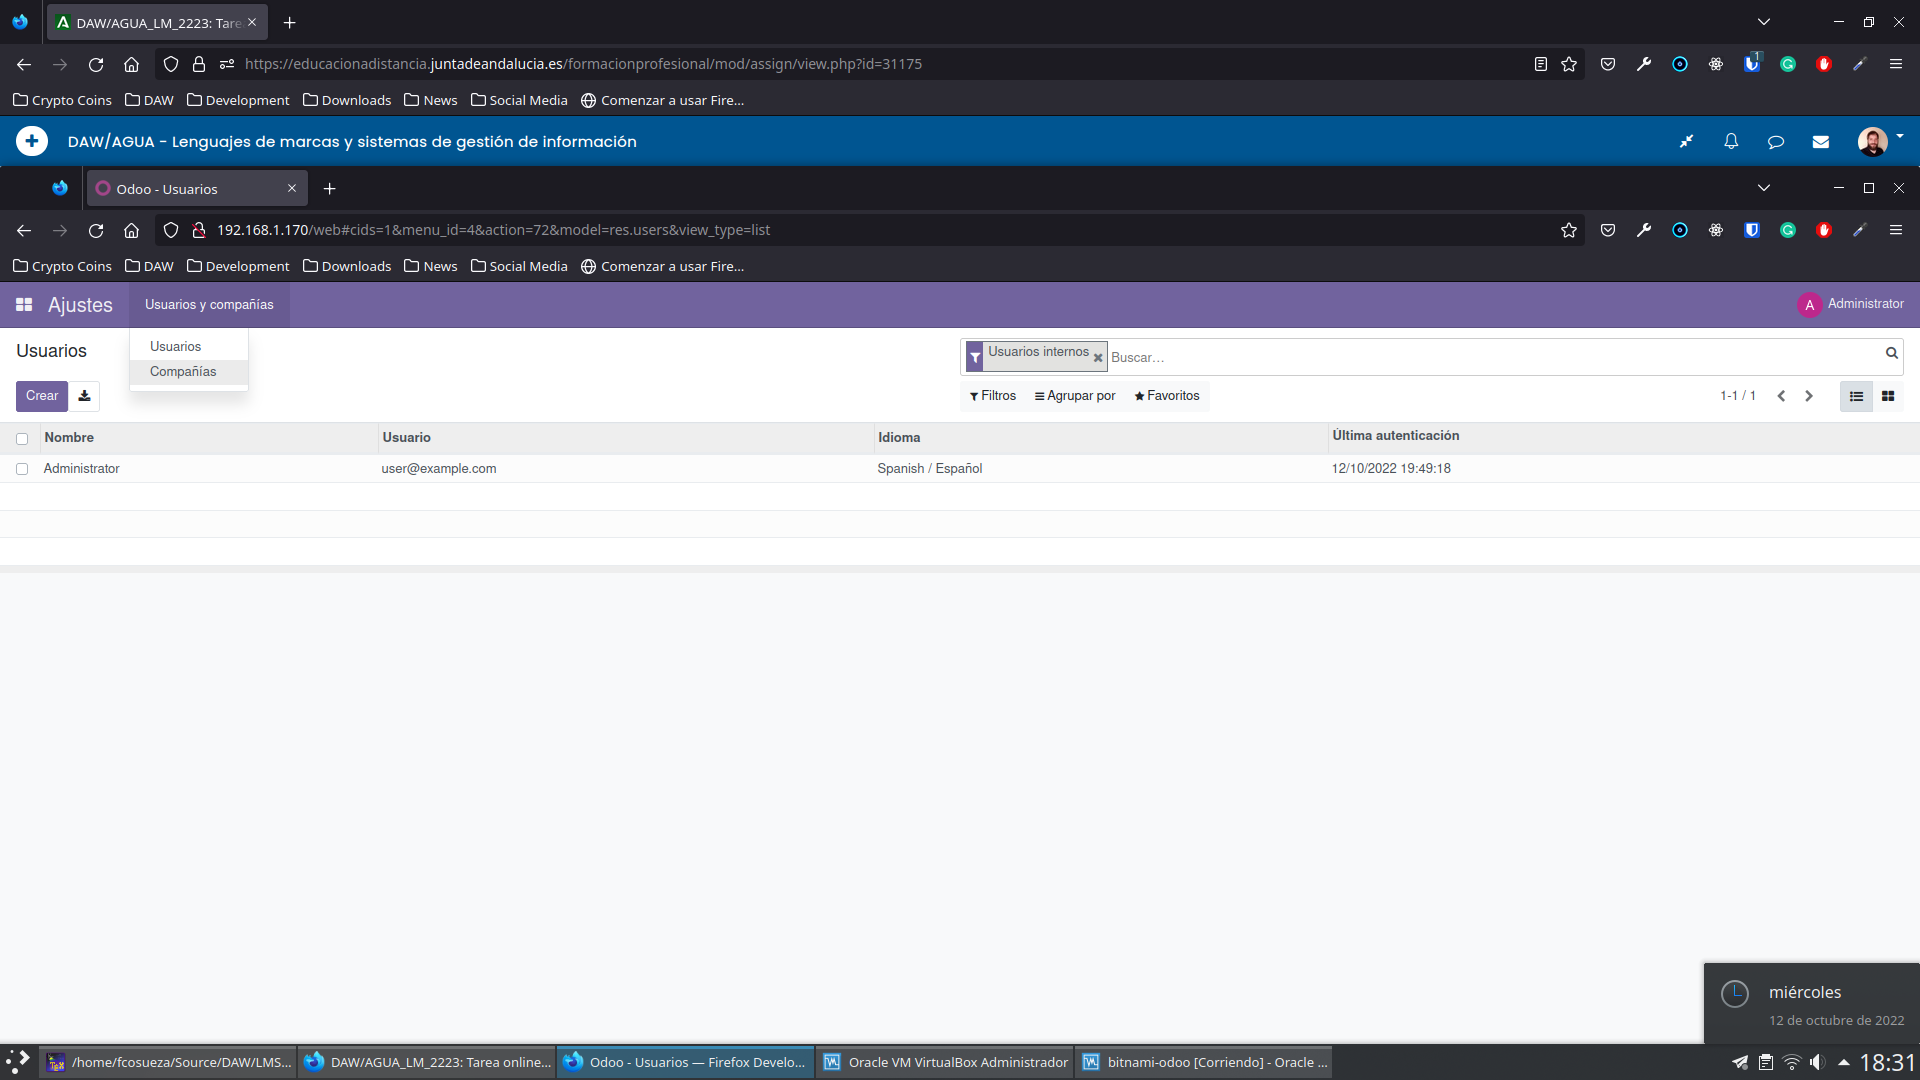
\includegraphics[scale=0.25]{companias.png}
        \caption{Lista de compañías añadidas en la aplicación}
    \end{figure}

    \vspace{5ex}

   \item Después de seleccionar la compañía, nos aparecerá una ficha con los datos de \textbf{My Company}, que es la que viene creada por defecto. Pulsamos en el botón \textbf{Editar}, arriba a la izquierda, y se desbloquearán los campos para poder cambiarlos con los datos que queramos. En nuestro caso, los de la compañía ficticia \textbf{Llegaya S.L}.

   \begin{figure}[ht]
       \centering
       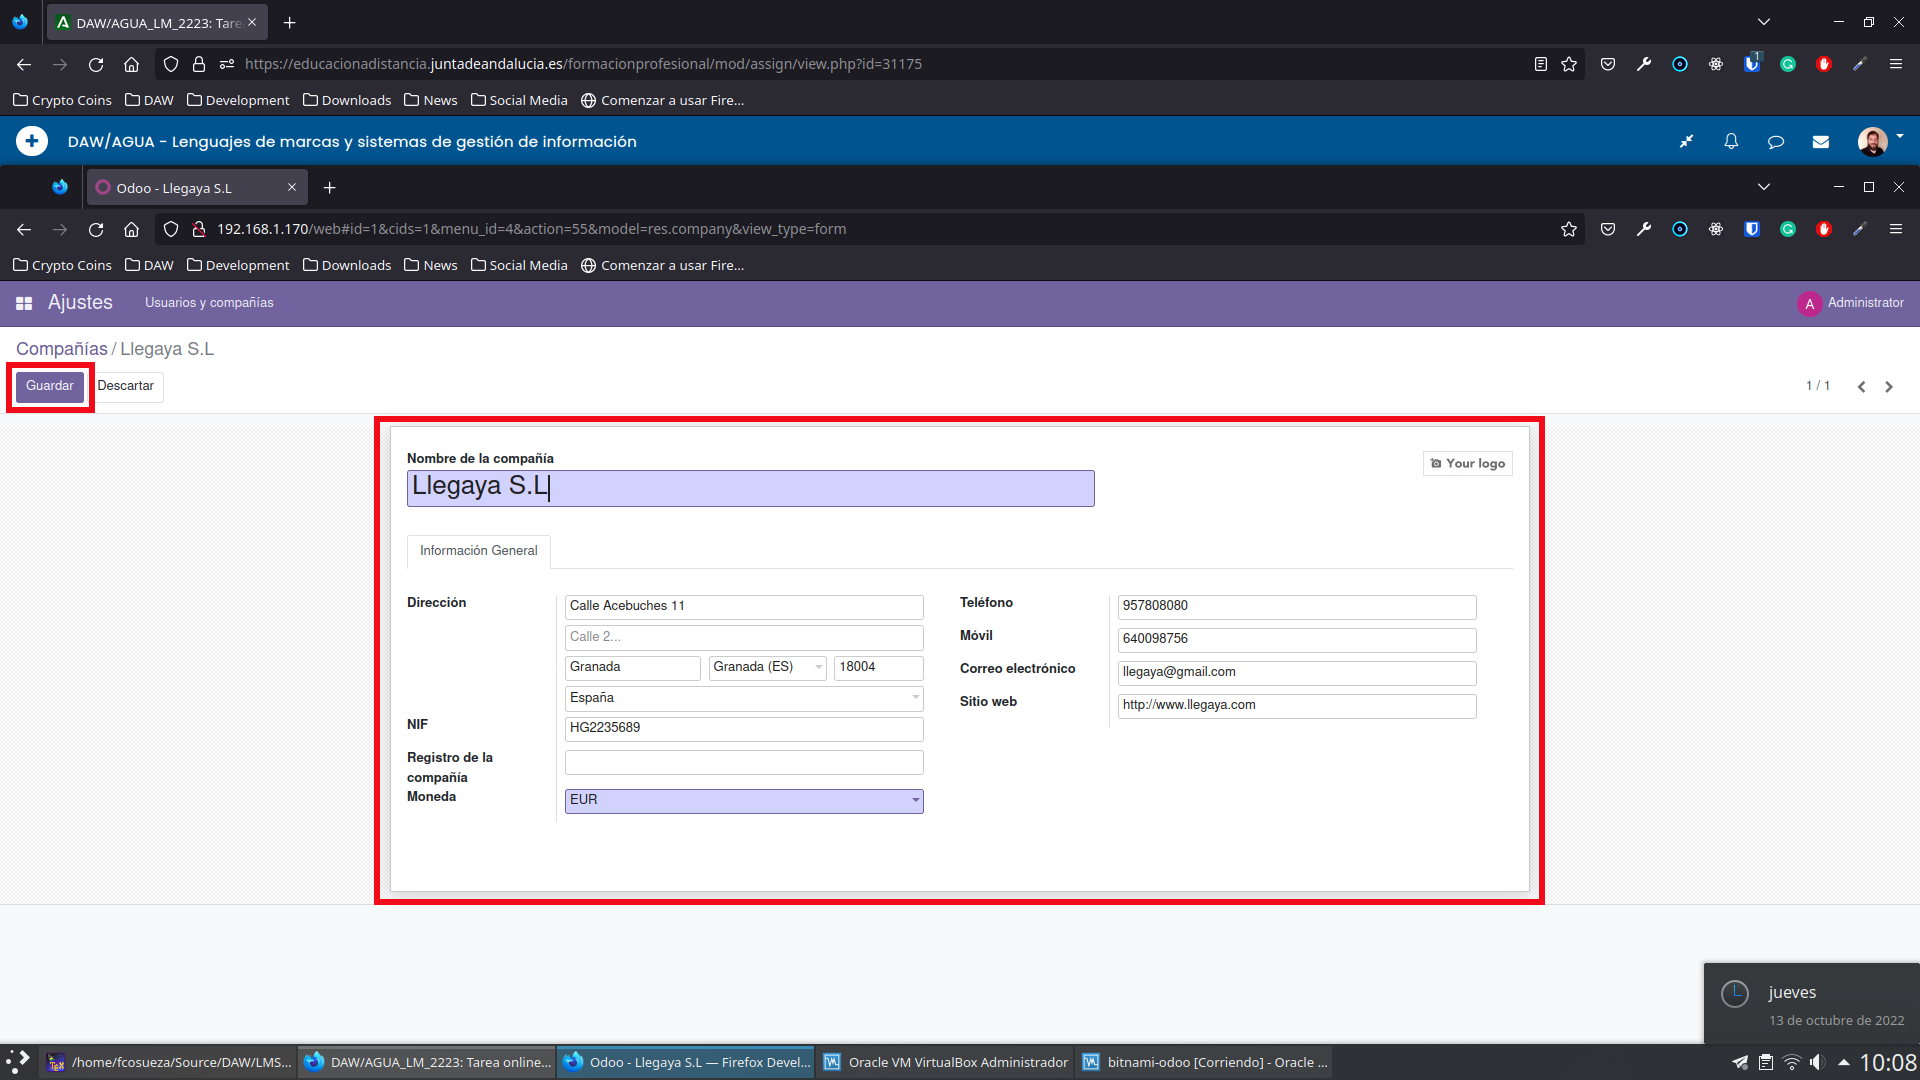
\includegraphics[scale=0.25]{companias-ficha.png}
       \caption{Ficha de la empresa editada}
   \end{figure}

   \item Por último pulsamos en \textbf{Guardar} y ya se habrán actualizado los datos de la compañía con los nuestros. En el caso de que queramos crear una empresa en vez de modificarla, solo deberemos pulsar en \textbf{Crear}, siendo el procedimiento el mismo.

   \begin{figure}[ht]
       \centering
       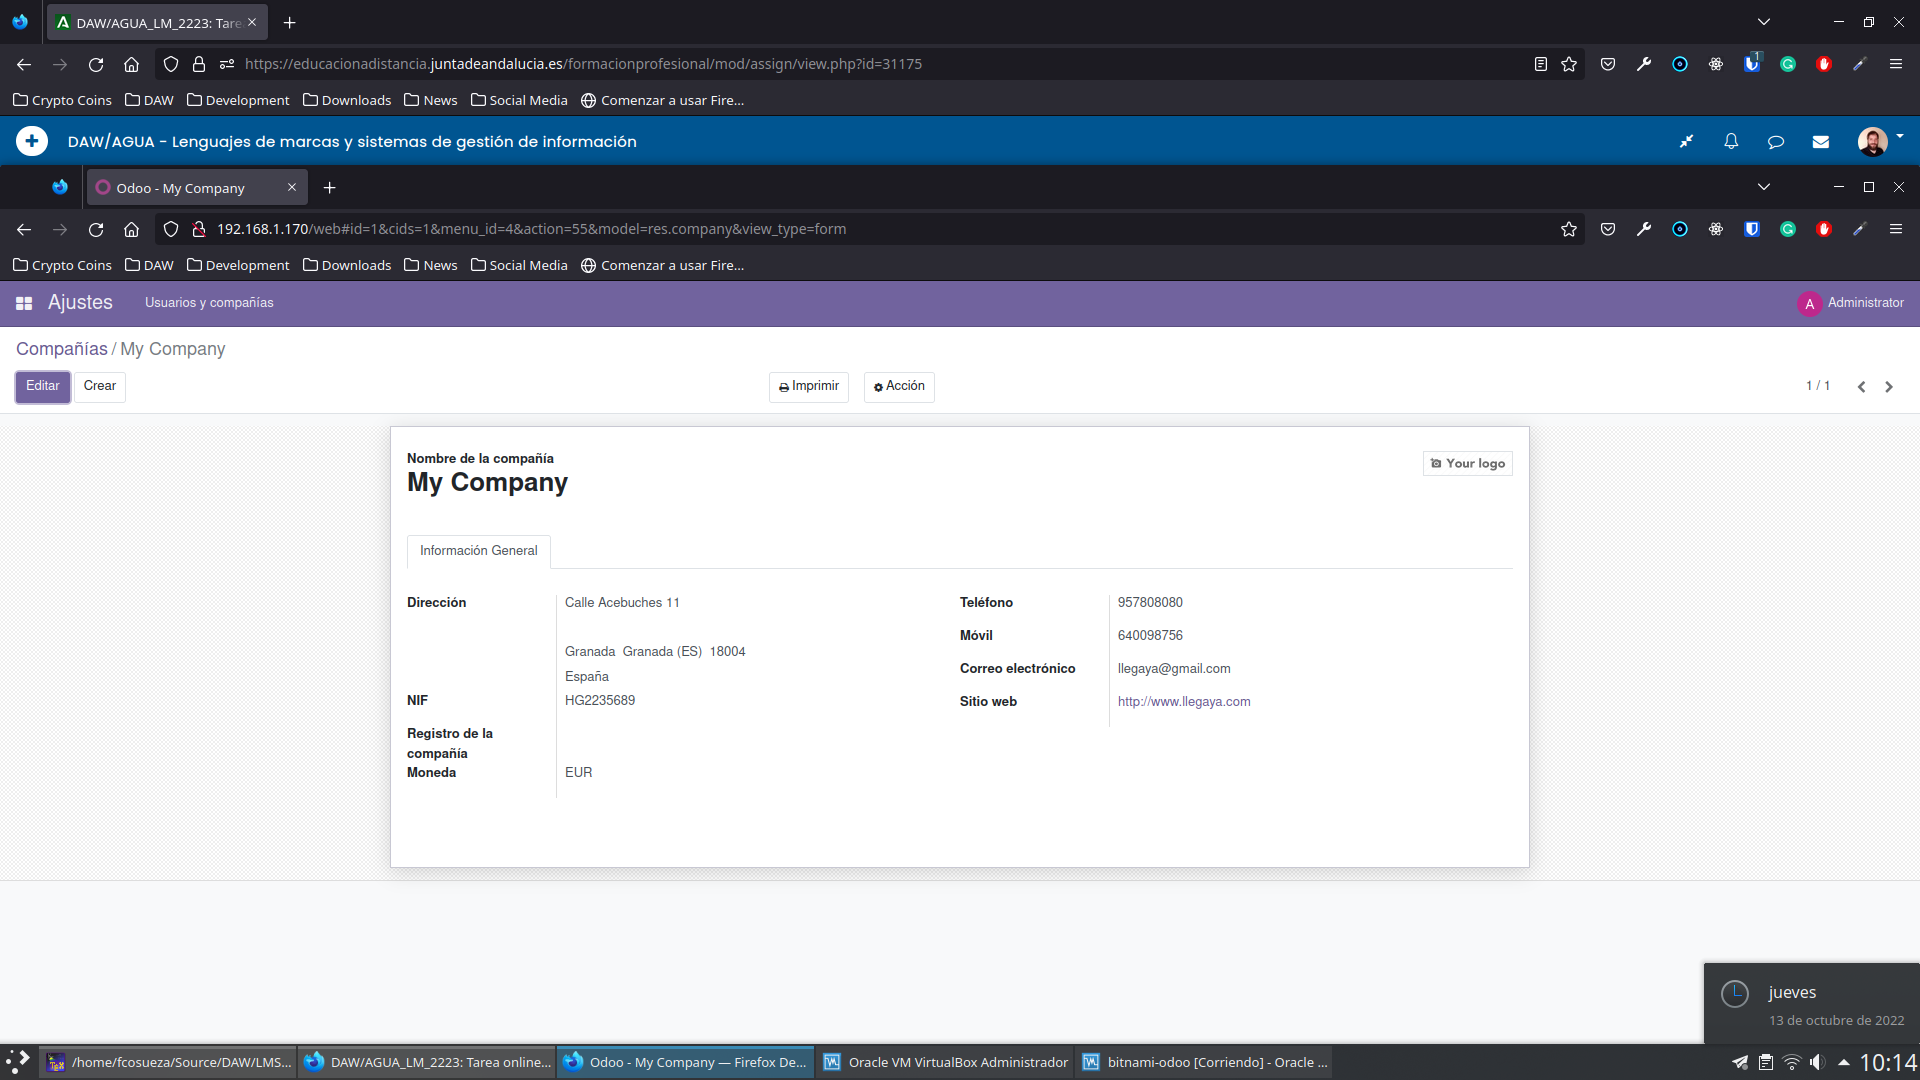
\includegraphics[scale=0.25]{compania-actualizada.png}
       \caption{Datos de la compañía actualizados}
   \end{figure}
\end{enumerate}

\subsection{Creación de Usuario}
A continuación, vamos a añadir dos usuarios al sistema, a parte del que ya viene por defecto. Para ello vamos a seguir los siguientes pasos.

\begin{enumerate}
    \item Desde la página que nos muestra la lista de usuarios, Figura \ref{fig:user}, pulsamos en el botón \textbf{Crear} en la parte superior izquierda.

     \begin{figure}[ht]
        \centering
        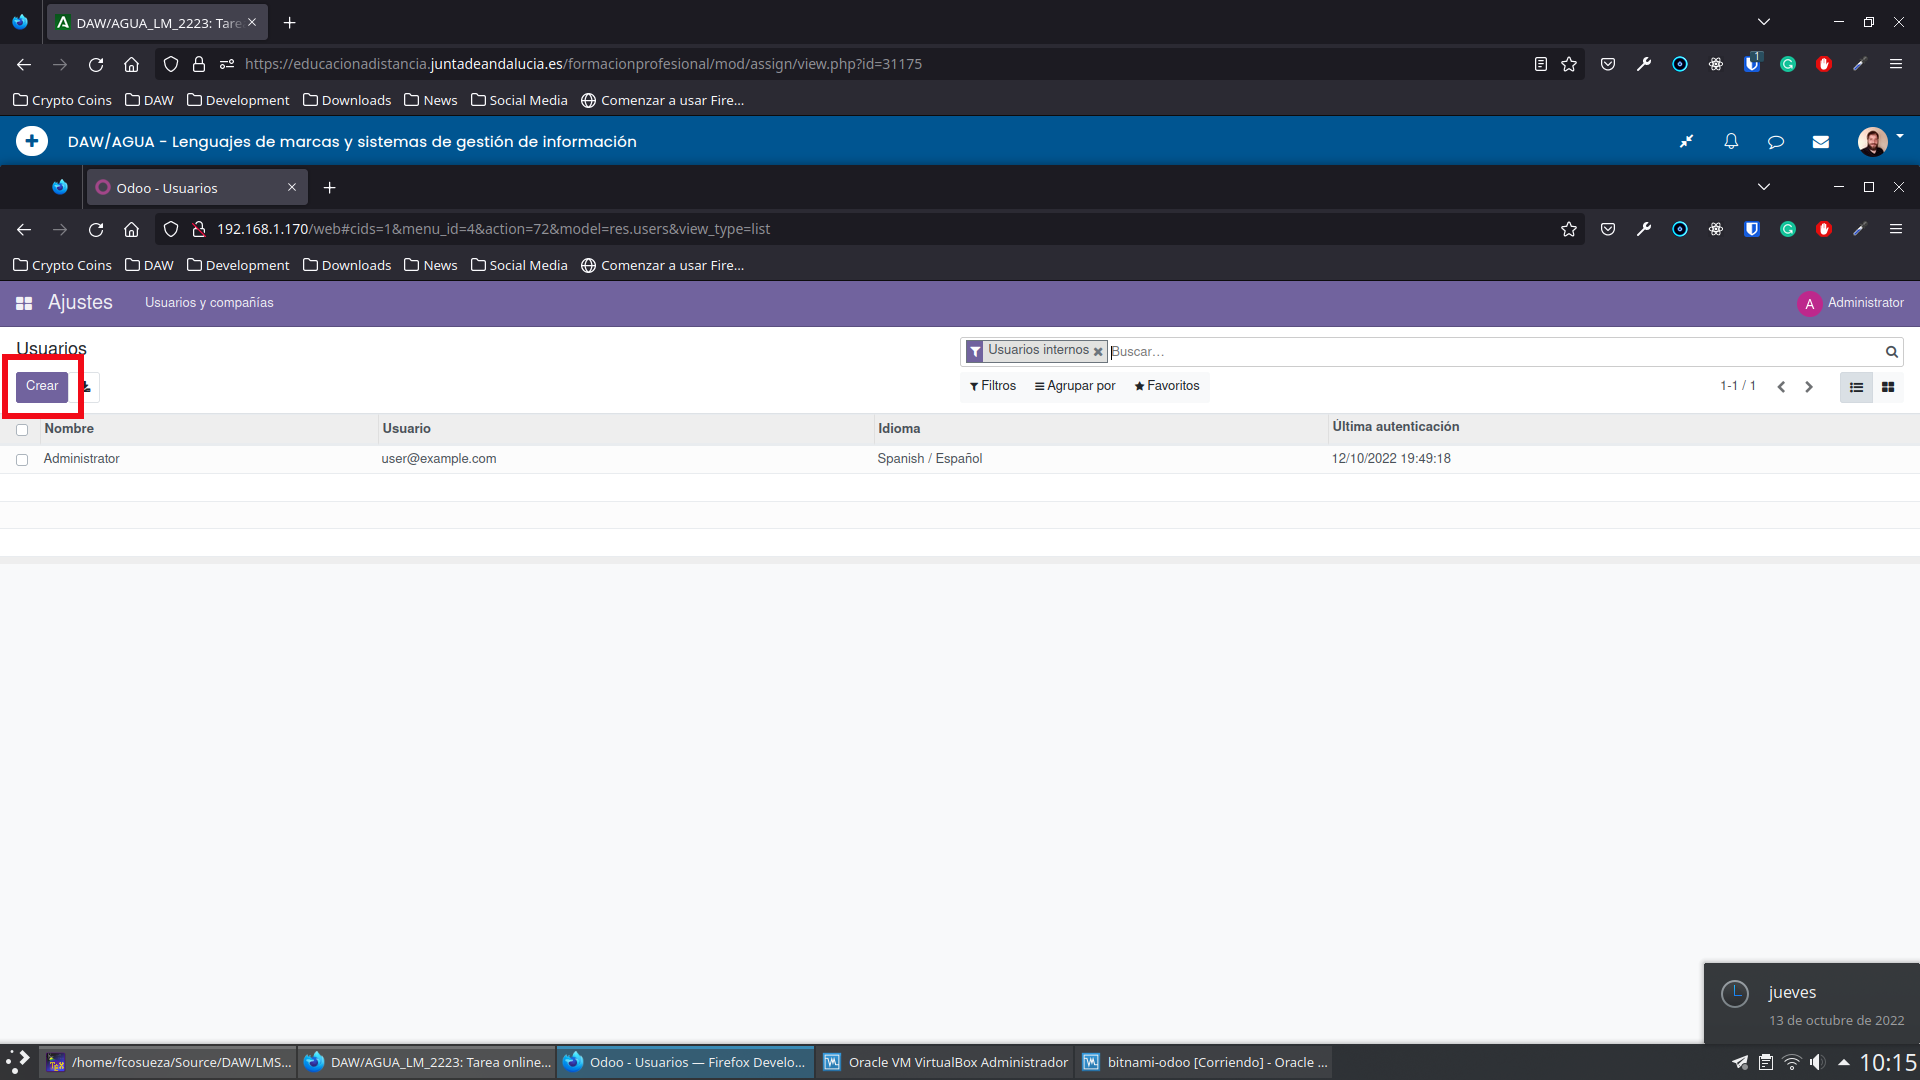
\includegraphics[scale=0.25]{usuarios-crear.png}
        \caption{Crear Usuario Nuevo}
    \end{figure}

    \item A continuación se nos mostrará una ficha de usuario que podemos editar. Introducimos el nombre y el correo de nuestro usuario. En la parte de abajo tenemos dos pestañas, en \textbf{Permisos de Usuario} podemos atribuirle permisos de administración al usuario, mientras que en \textbf{Preferencias} podremos cambiar opciones como la \textbf{zona horaria}, \textbf{idioma} o la \textbf{firma de correo electrónico}. Una vez introducidos los datos, pulsamos en Guardar y el usuario se habrá creado.

    \begin{figure}[ht]
        \centering
        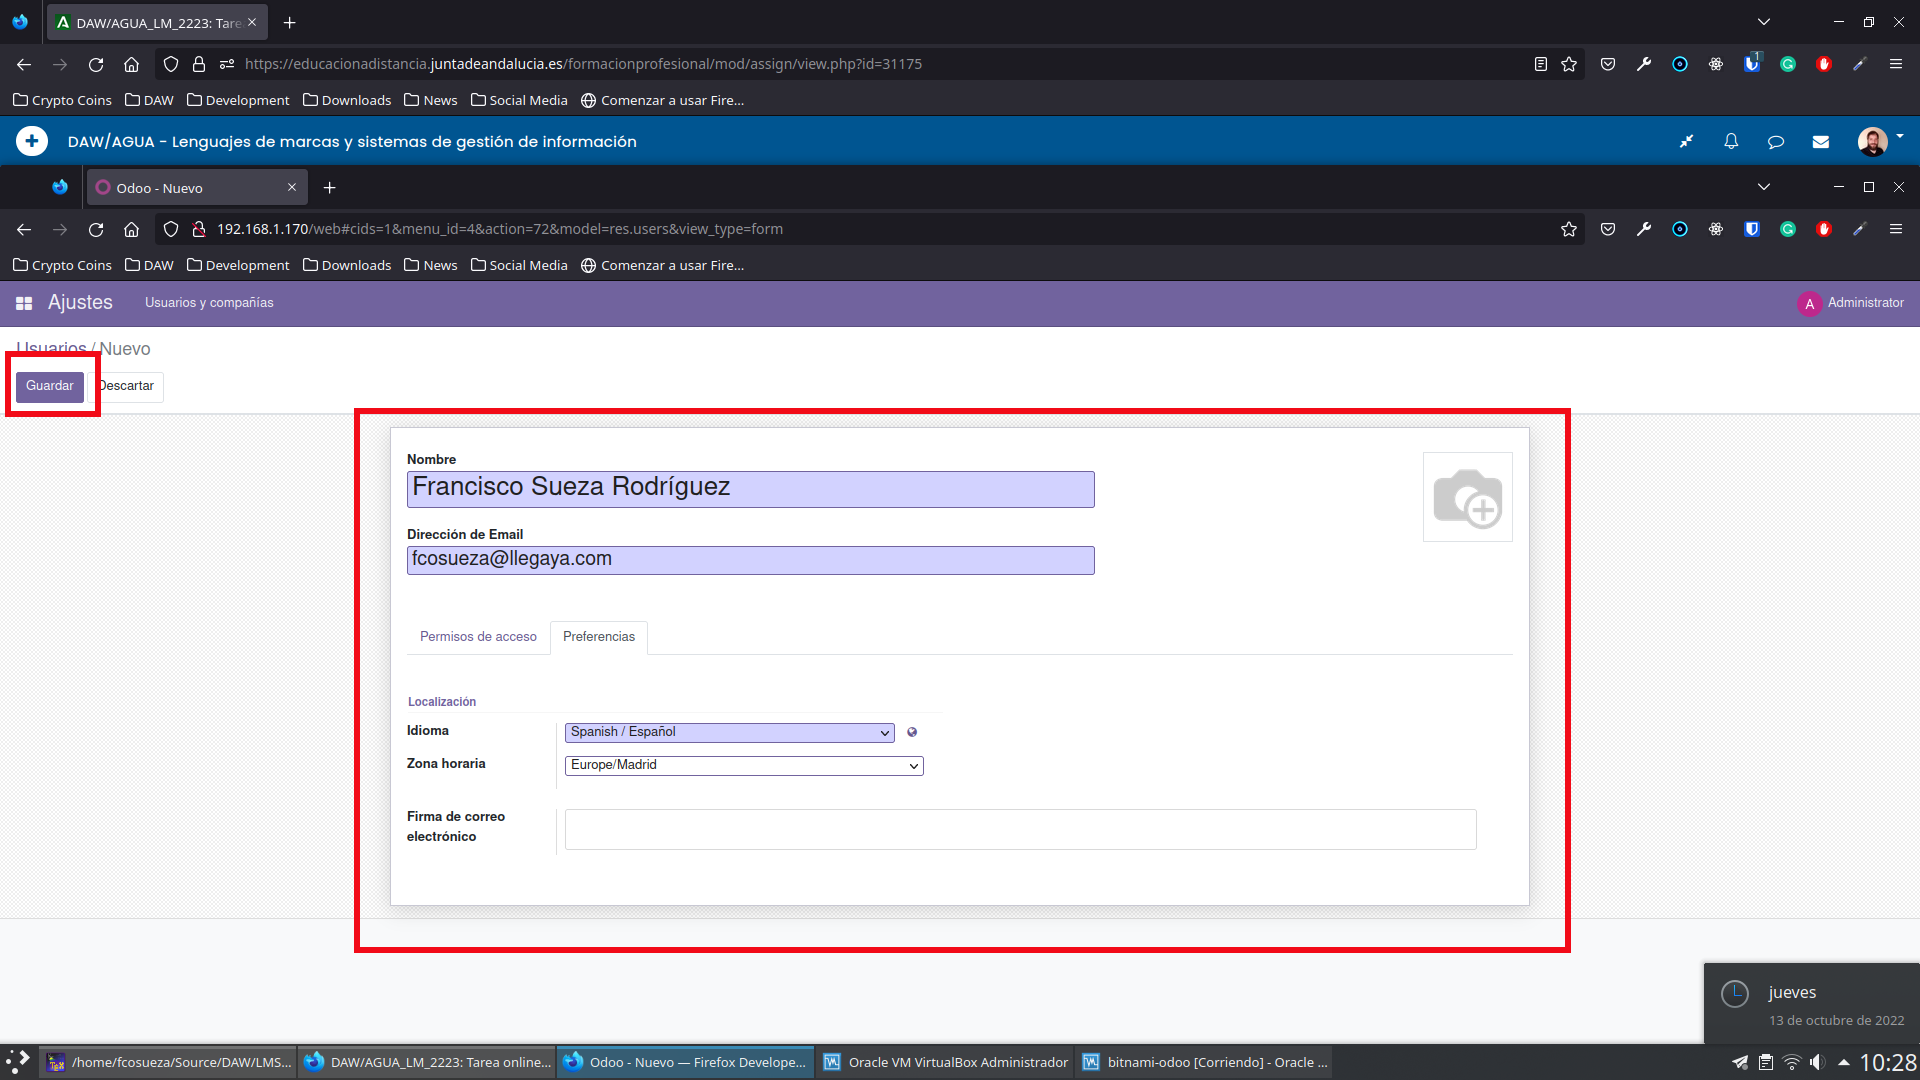
\includegraphics[scale=0.25]{usuario-crear-datos.png}
        \caption{Introducción de datos de usuario nuevo}
    \end{figure}
\end{enumerate}

Se han creado dos usuarios, uno con los datos del alumno (los míos) y otro con los datos del profesor, siguiendo el procedimiento descrito, como se puede ver en la siguiente captura.

\begin{figure}[ht]
    \centering
    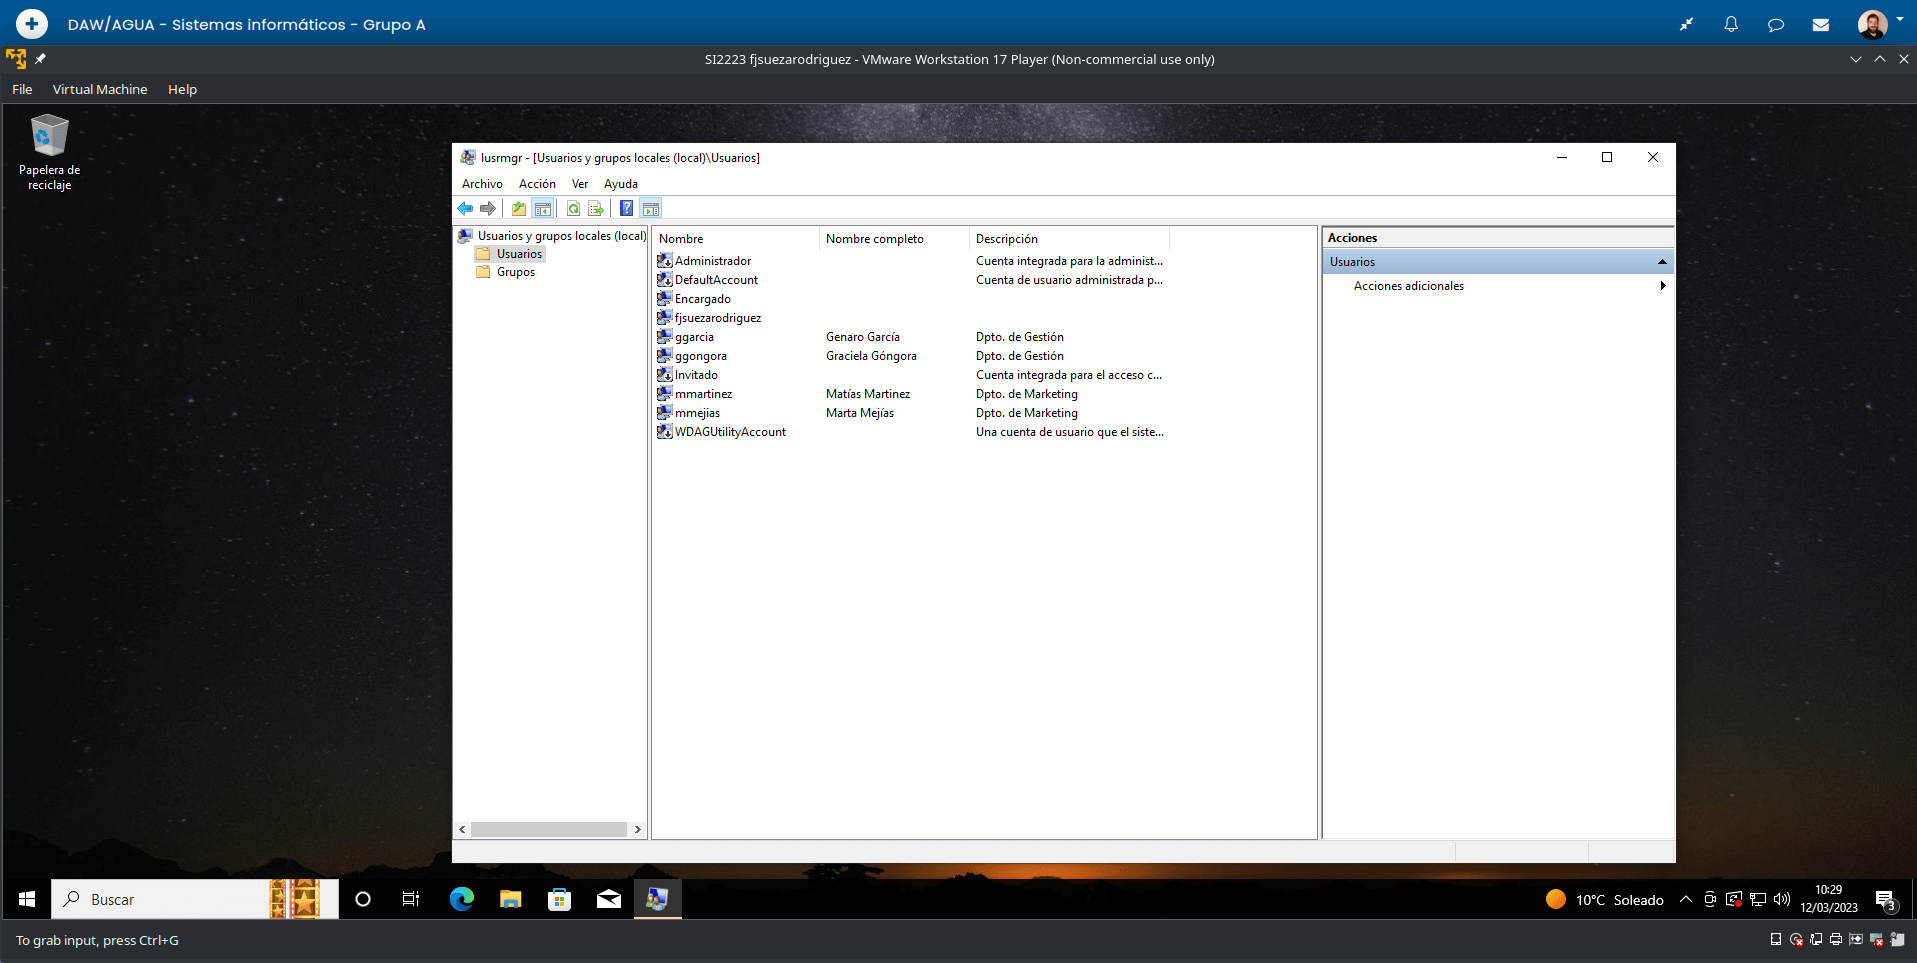
\includegraphics[scale=0.25]{usuarios-creados.png}
    \caption{Lista con los usuarios creados}
\end{figure}

\section{Instalación de Módulos y Generación de Informes}
En esta sección vamos a instalar un módulo de Odoo, en concreto el módulo \textbf{Inventario}, para posteriormente \textbf{crear tres paquetes} diferentes y generar un informe de los paquetes creados.

\subsection{Instalación de Módulo Inventario}
La instalación de módulos se realiza de forma muy sencilla. Desde la página principal de Odoo, donde se muestran todas las aplicaciones, solo tenemos que pulsar en el botón \textbf{Instalar} del módulo que queramos y el proceso de hará de forma automática.

\begin{figure}[ht]
    \centering
    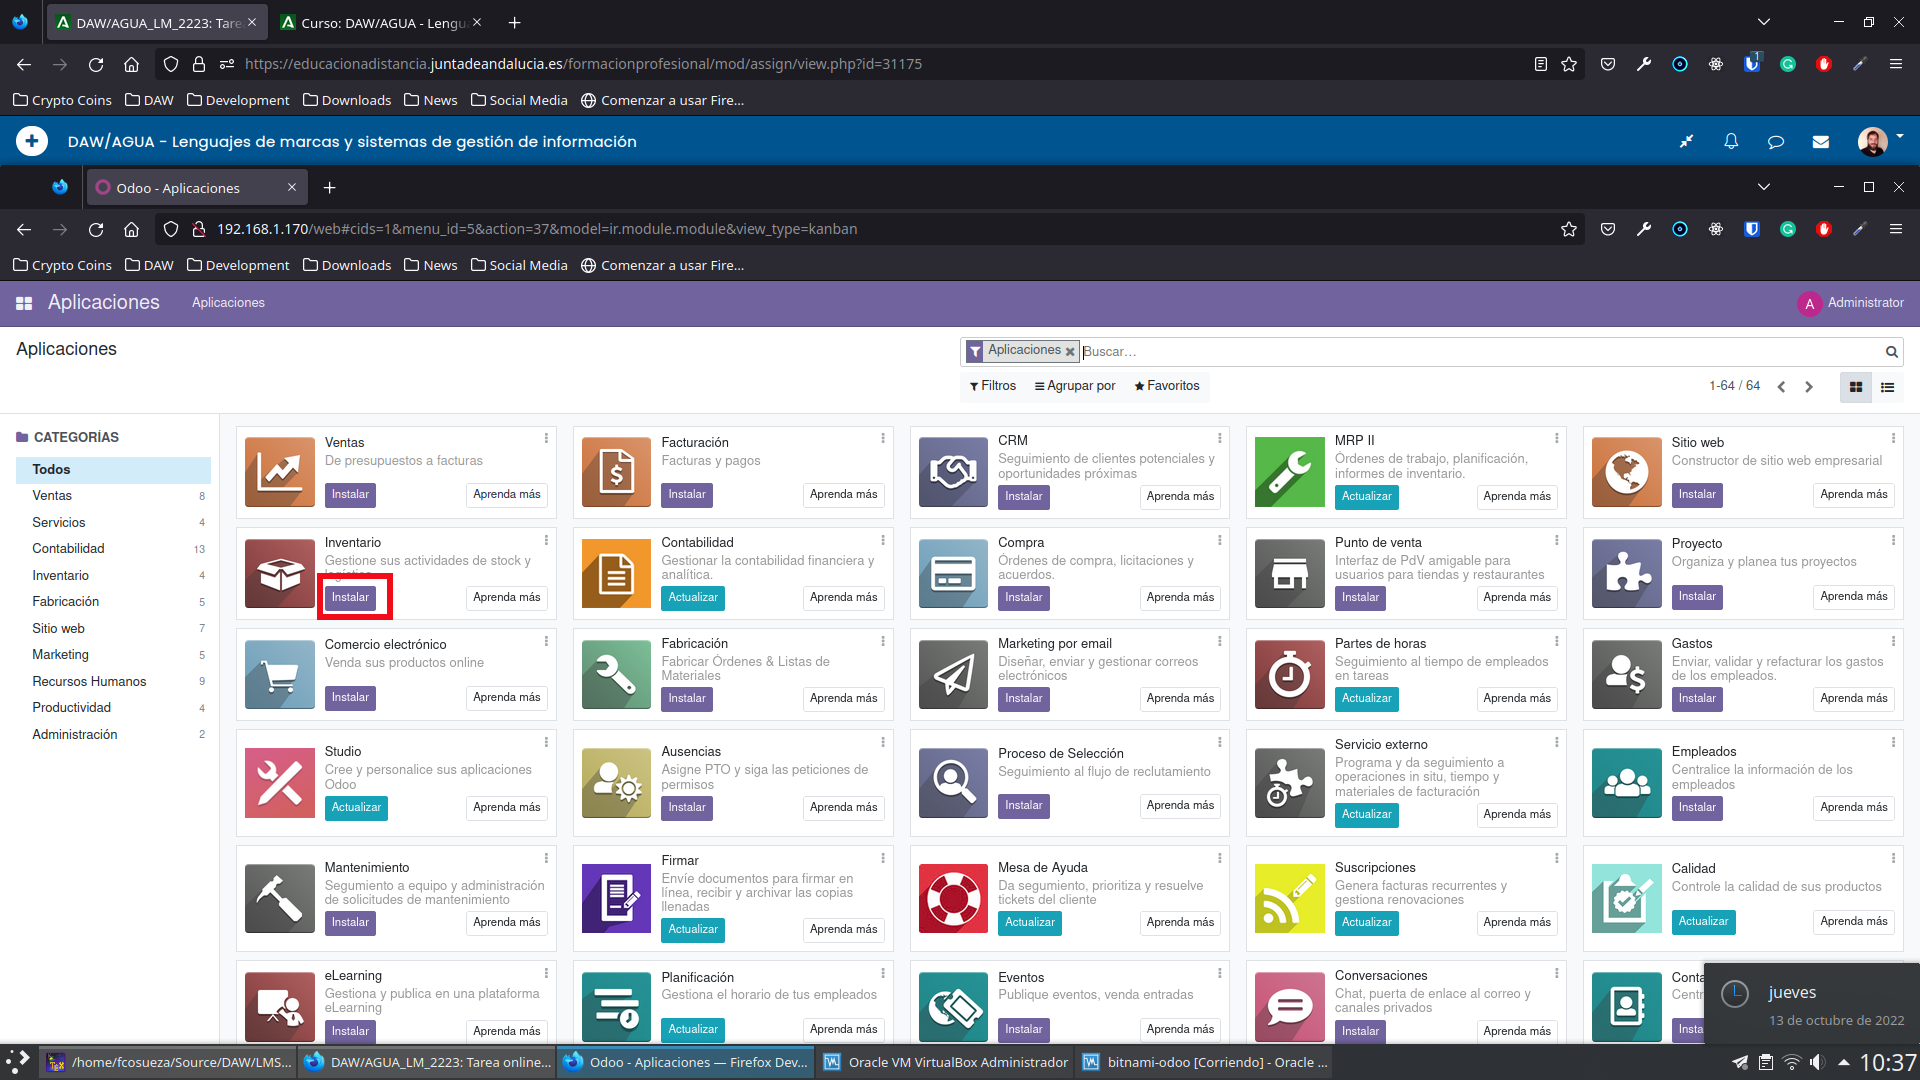
\includegraphics[scale=0.25]{instalar-modulo.png}
    \caption{Instalación de módulo Inventario}
\end{figure}

Una vez hayamos instalado el módulo, y siendo este el primero que instalamos, se habrá añadido automáticamente el \textbf{módulo Conversaciones}, que se usa para comunicaciones internas y para obtener ayuda a través de un ChatBot, \textbf{Odoobot}. Además, ya podremos acceder desde el menú desplegable tanto al módulo Inventario como a Conversaciones.

\begin{figure}[ht]
    \centering
    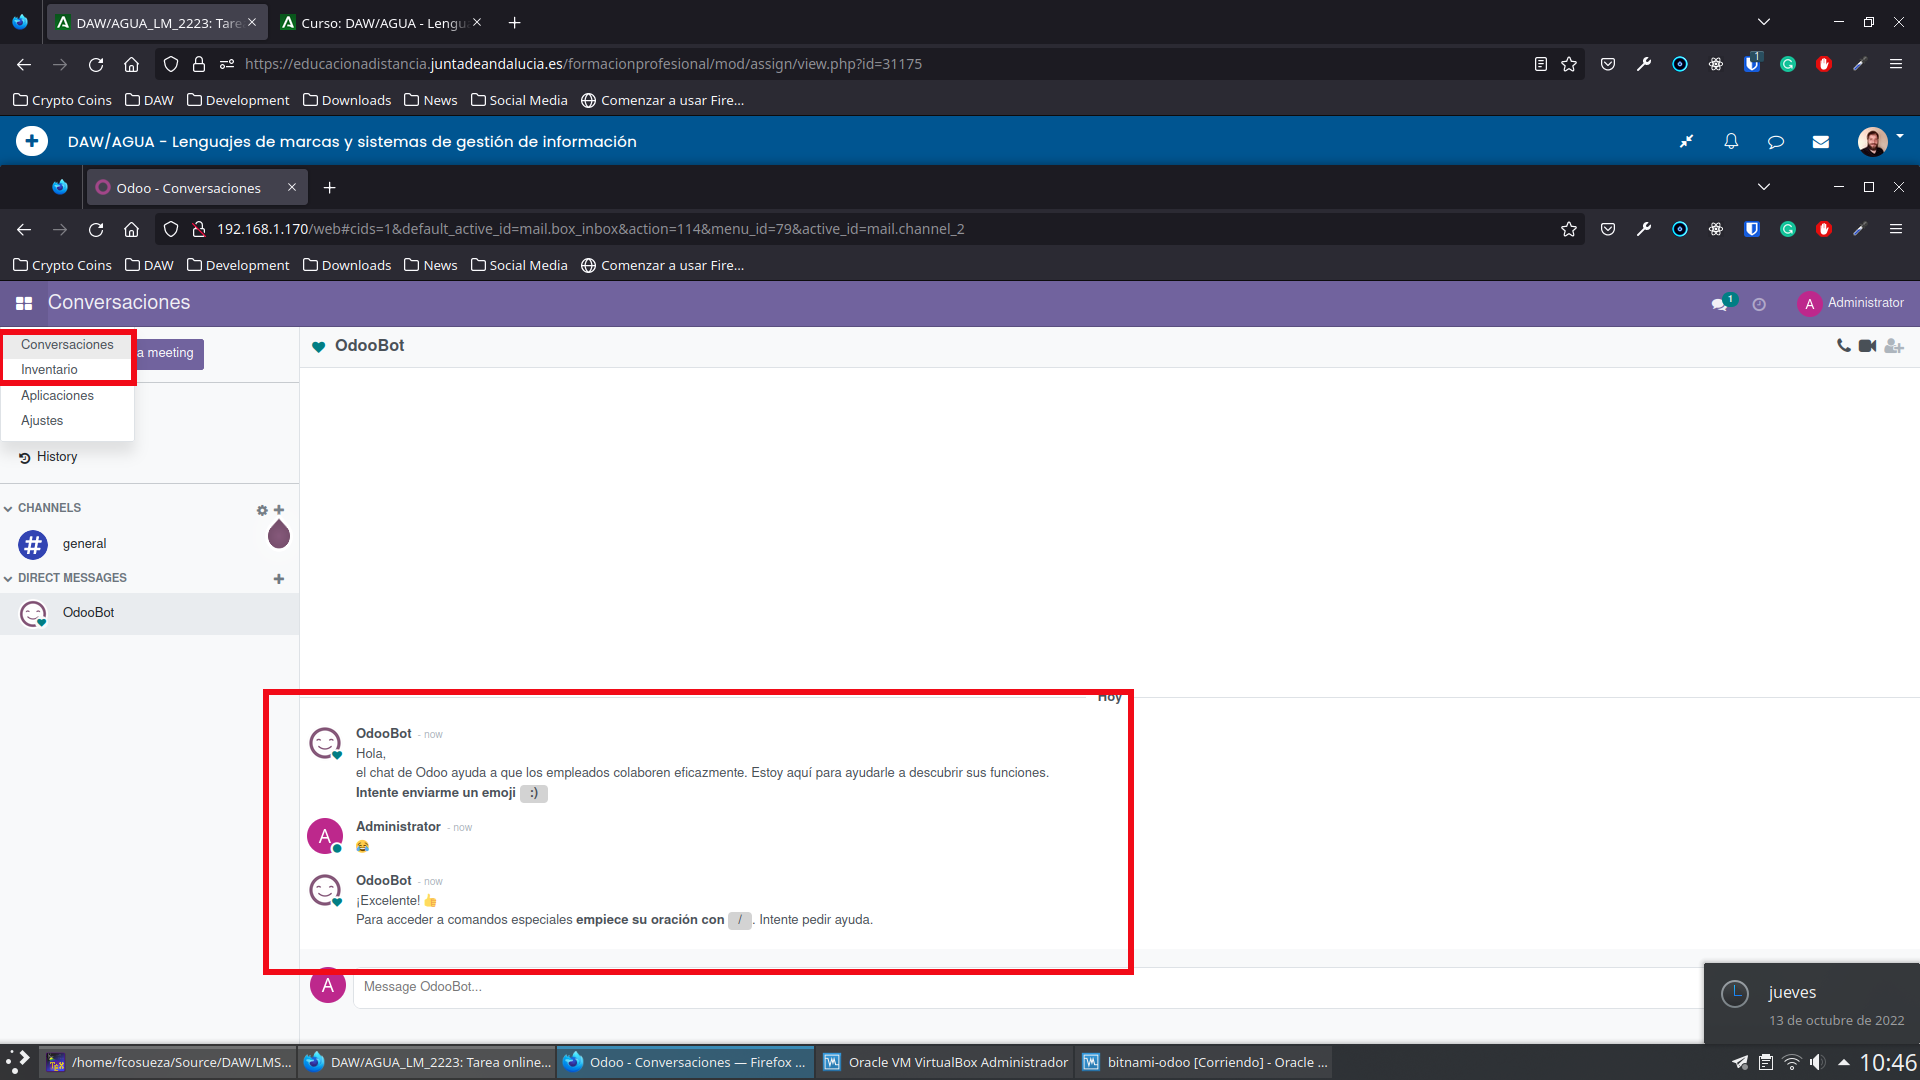
\includegraphics[scale=0.25]{odoobot.png}
    \caption{Odoobot en el módulo Conversaciones}
\end{figure}

\subsection{Creación de Productos}
Una vez instalado el módulo Inventario, podemos seleccionarlo desde el menú desplegable. Se nos mostrará la página con información general del módulo, donde podemos ver las \textbf{Recepciones}, \textbf{Expediciones} y \textbf{Devoluciones} (Returns) de los productos que tenemos en el inventario. Ahora mismo se muestra vacío, ya que no tenemos ningún producto almacenado.

\begin{figure}[ht]
    \centering
    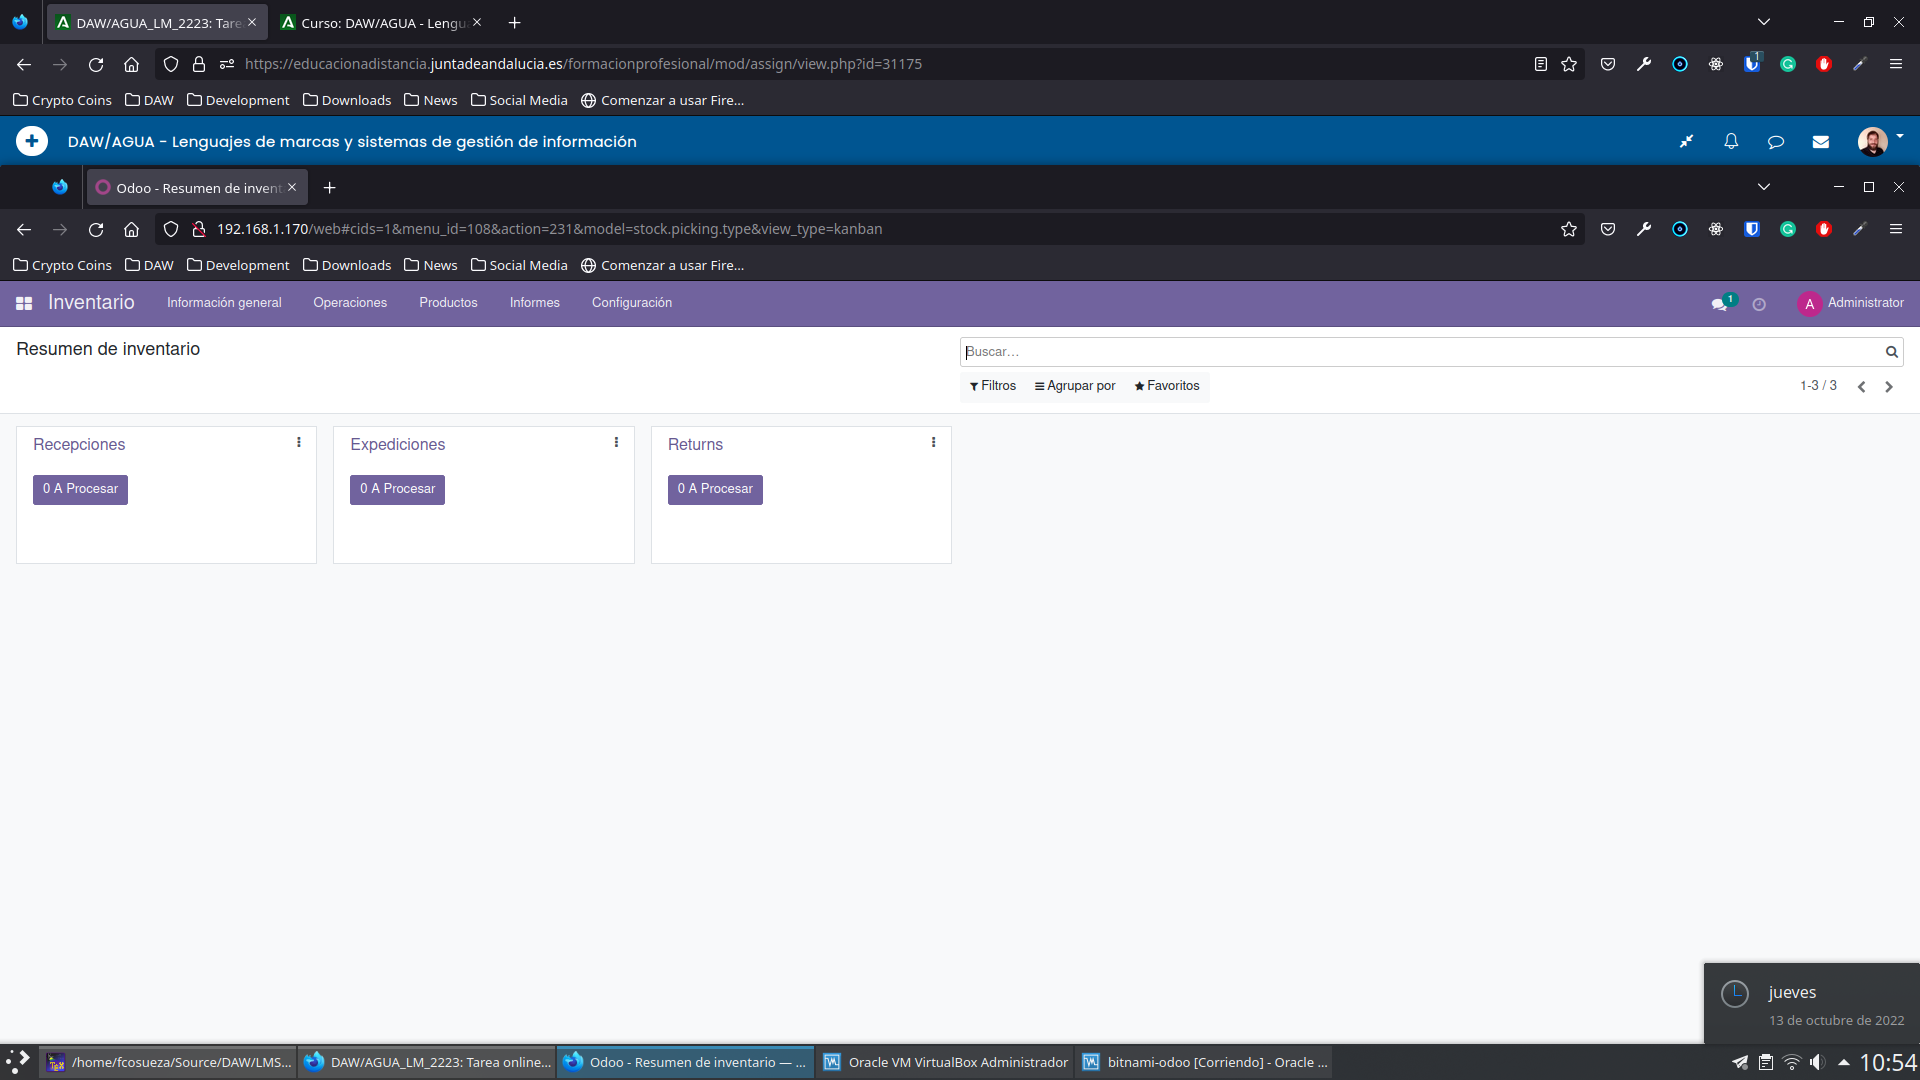
\includegraphics[scale=0.25]{inventario-info.png}
    \caption{Página principal del módulo Inventario}
\end{figure}

Para crear los paquetes diferentes que se nos piden, deberemos añadir 3 productos con una cantidad de 1 cada uno. Para hacerlo, debemos seguir los siguientes pasos.

\vspace{5ex}

\begin{enumerate}
    \item En primer lugar, pulsamos en la barra superior, en el menú \textbf{Productos} y seleccionamos la opción \textbf{Productos}. Esto nos llevará a una página donde se mostrarán todos los productos almacenados. Ahora mismo vacía.

    \begin{figure}[ht]
        \centering
        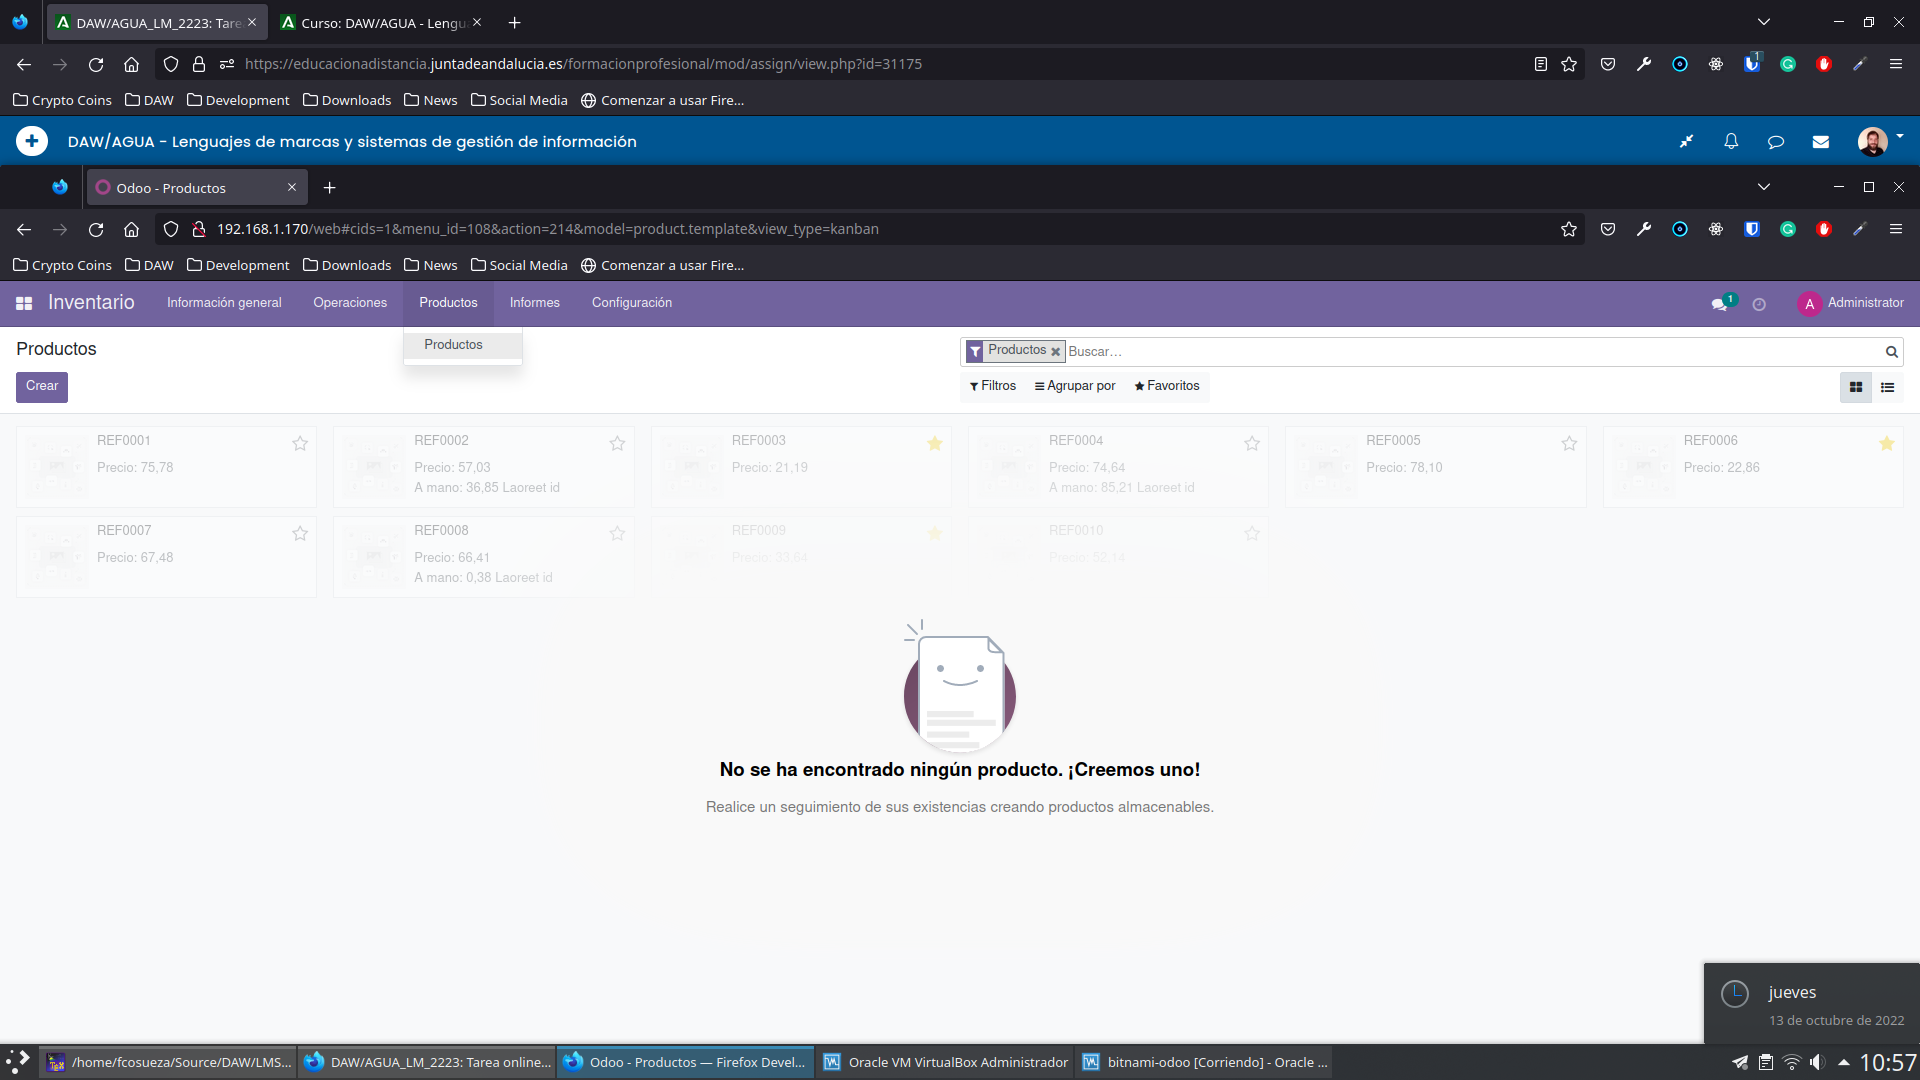
\includegraphics[scale=0.25]{inventario-productos.png}
        \caption{Apartado Productos del modulo Inventario}
    \end{figure}

    \item A continuación pulsamos el botón \textbf{Crear}, arriba a la izquierda, y se nos mostrará una ficha editable con diferente información que debemos rellenar sobre nuestro producto, como el \textbf{nombre}, \textbf{precio de venta}, \textbf{coste}, etc.. Si pulsamos en la pestaña \textbf{Inventario} podremos añadir mas información como el \textbf{responsable de su almacenamiento}, \textbf{peso}, \textbf{volumen}, etc..

    Arriba a la derecha, también tenemos varias opciones, como \textbf{Imprimir etiquetas}, \textbf{Actualizar cantidad} y \textbf{Reabastecer}. Nosotros en primer lugar vamos a meter los datos de nuestro producto, en este caso, \textbf{Paquete Grande}.

    \begin{figure}[ht]
        \centering
        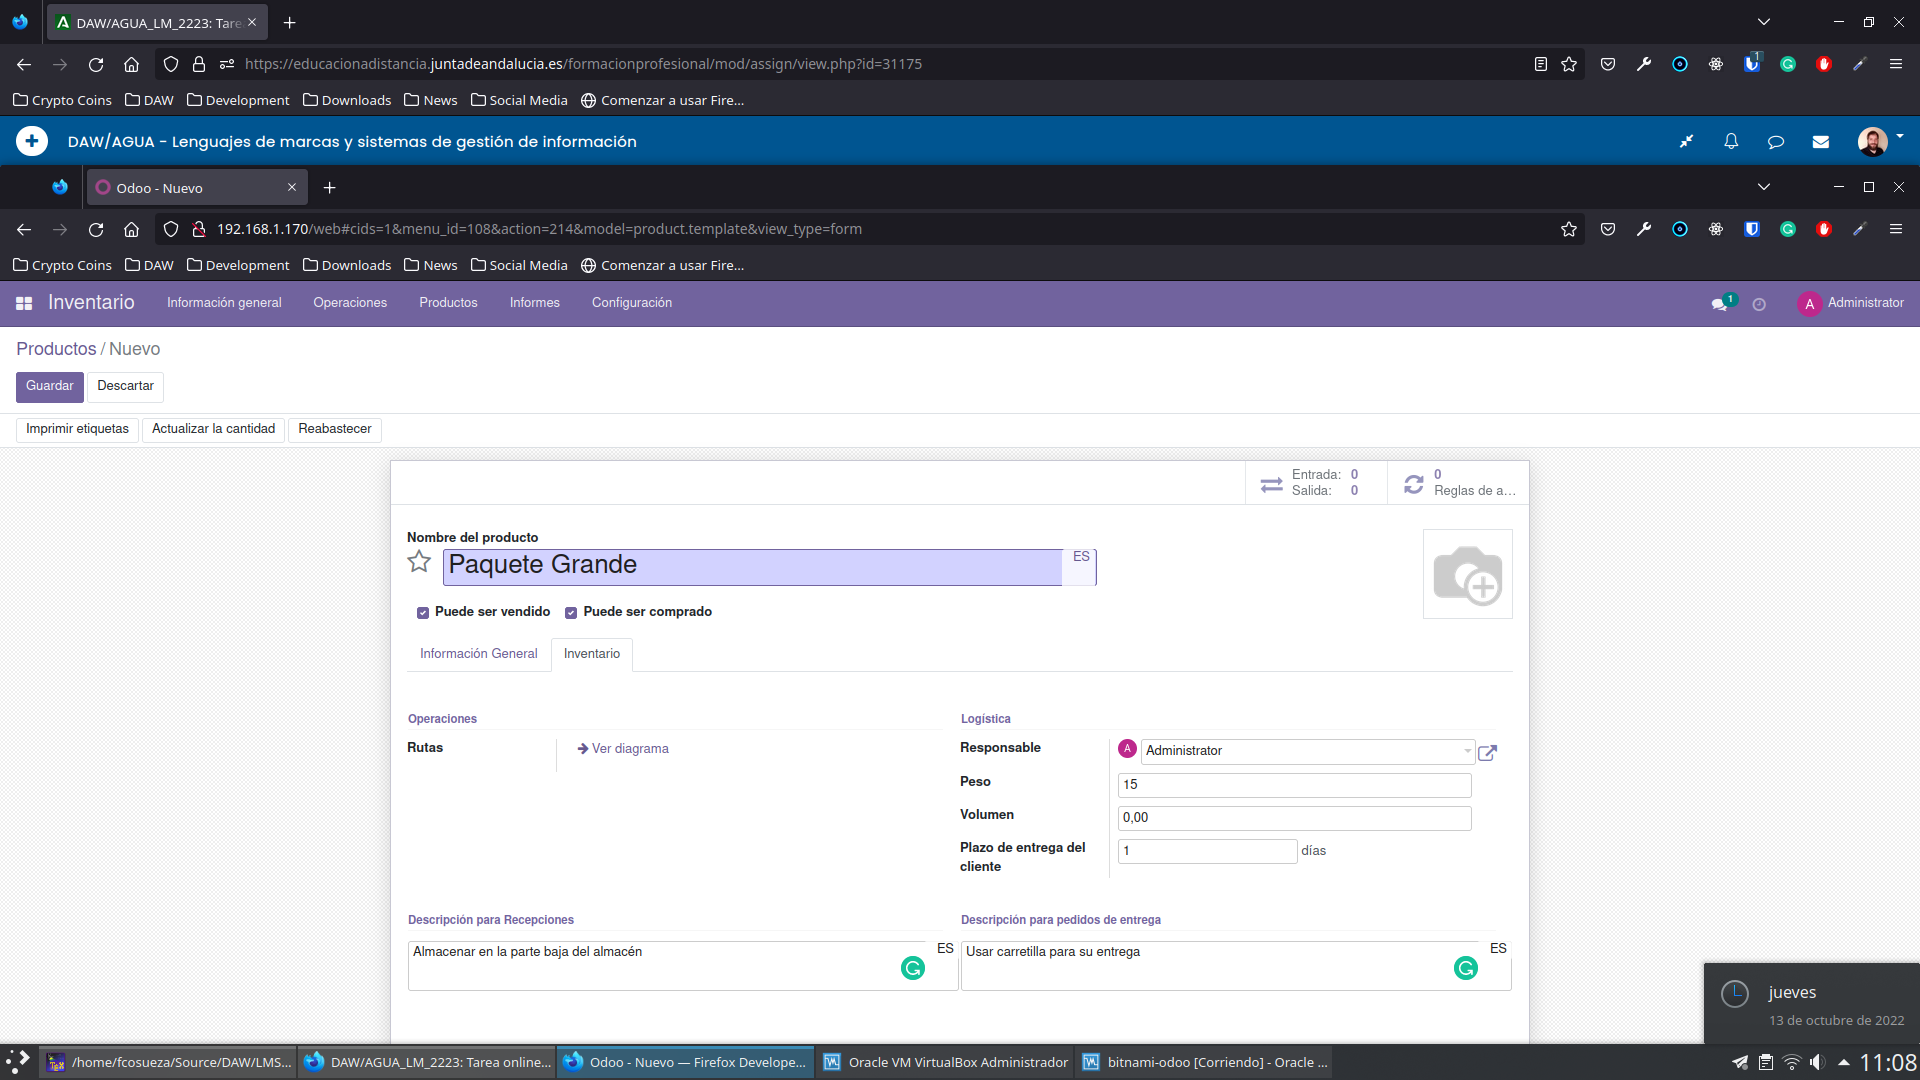
\includegraphics[scale=0.25]{inventario-paquete.png}
        \caption{Formulario de creación de Producto}
    \end{figure}

    \vspace{5ex}

    \item Una vez introducidos los datos vamos a actualizar la cantidad de tenemos en stock, una unidad en este caso. Para ello pulsamos en la opción \textbf{Actualizar cantidad} e introducimos la cantidad deseada y pulsamos en \textbf{Aplicar} para actualizar la información sobre el producto.

    \begin{figure}[ht]
        \centering
        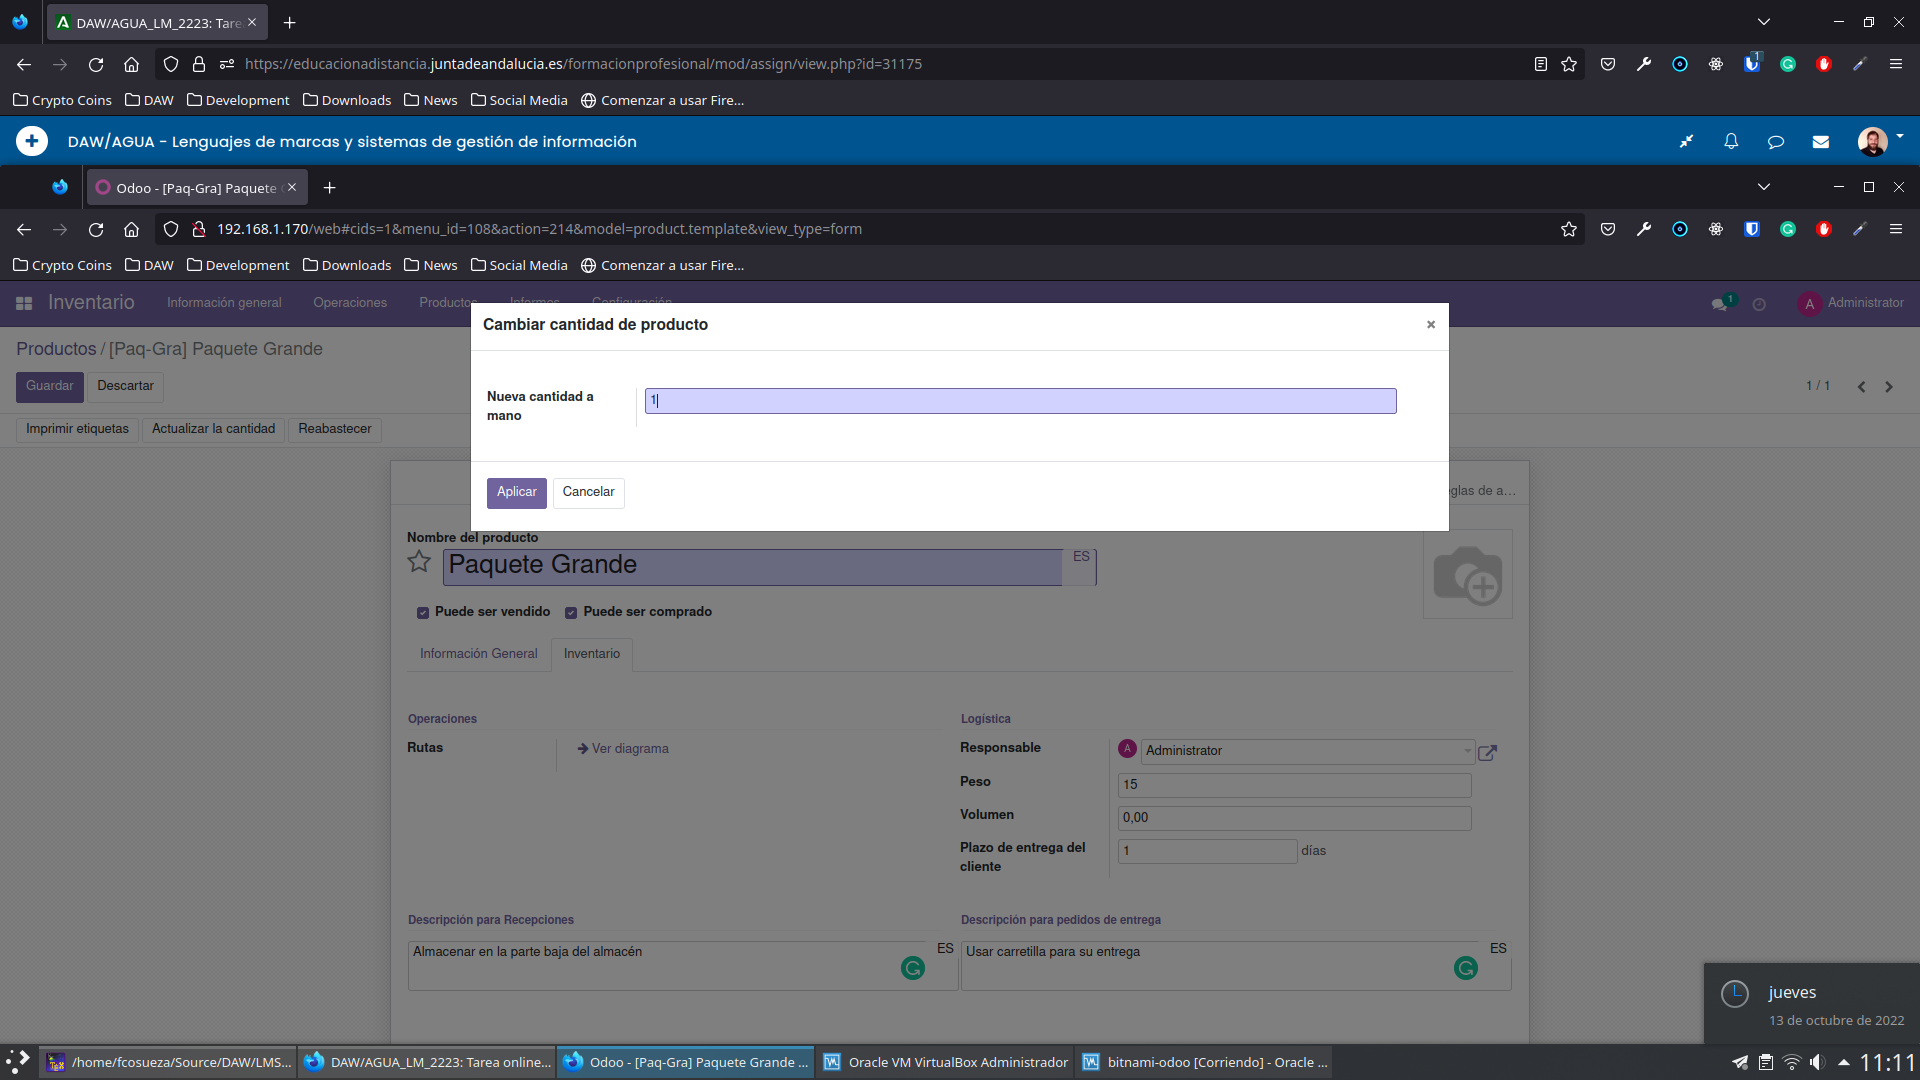
\includegraphics[scale=0.25]{inventario-paquete-cantidad.png}
        \caption{Actualización cantidad de producto}
    \end{figure}

    \item Por último, pulsamos en \textbf{Guardar} y nuestro producto se habrá creado correctamente. Ya podemos visualizarlo en la página principal de Productos.

    \begin{figure}[ht]
        \centering
        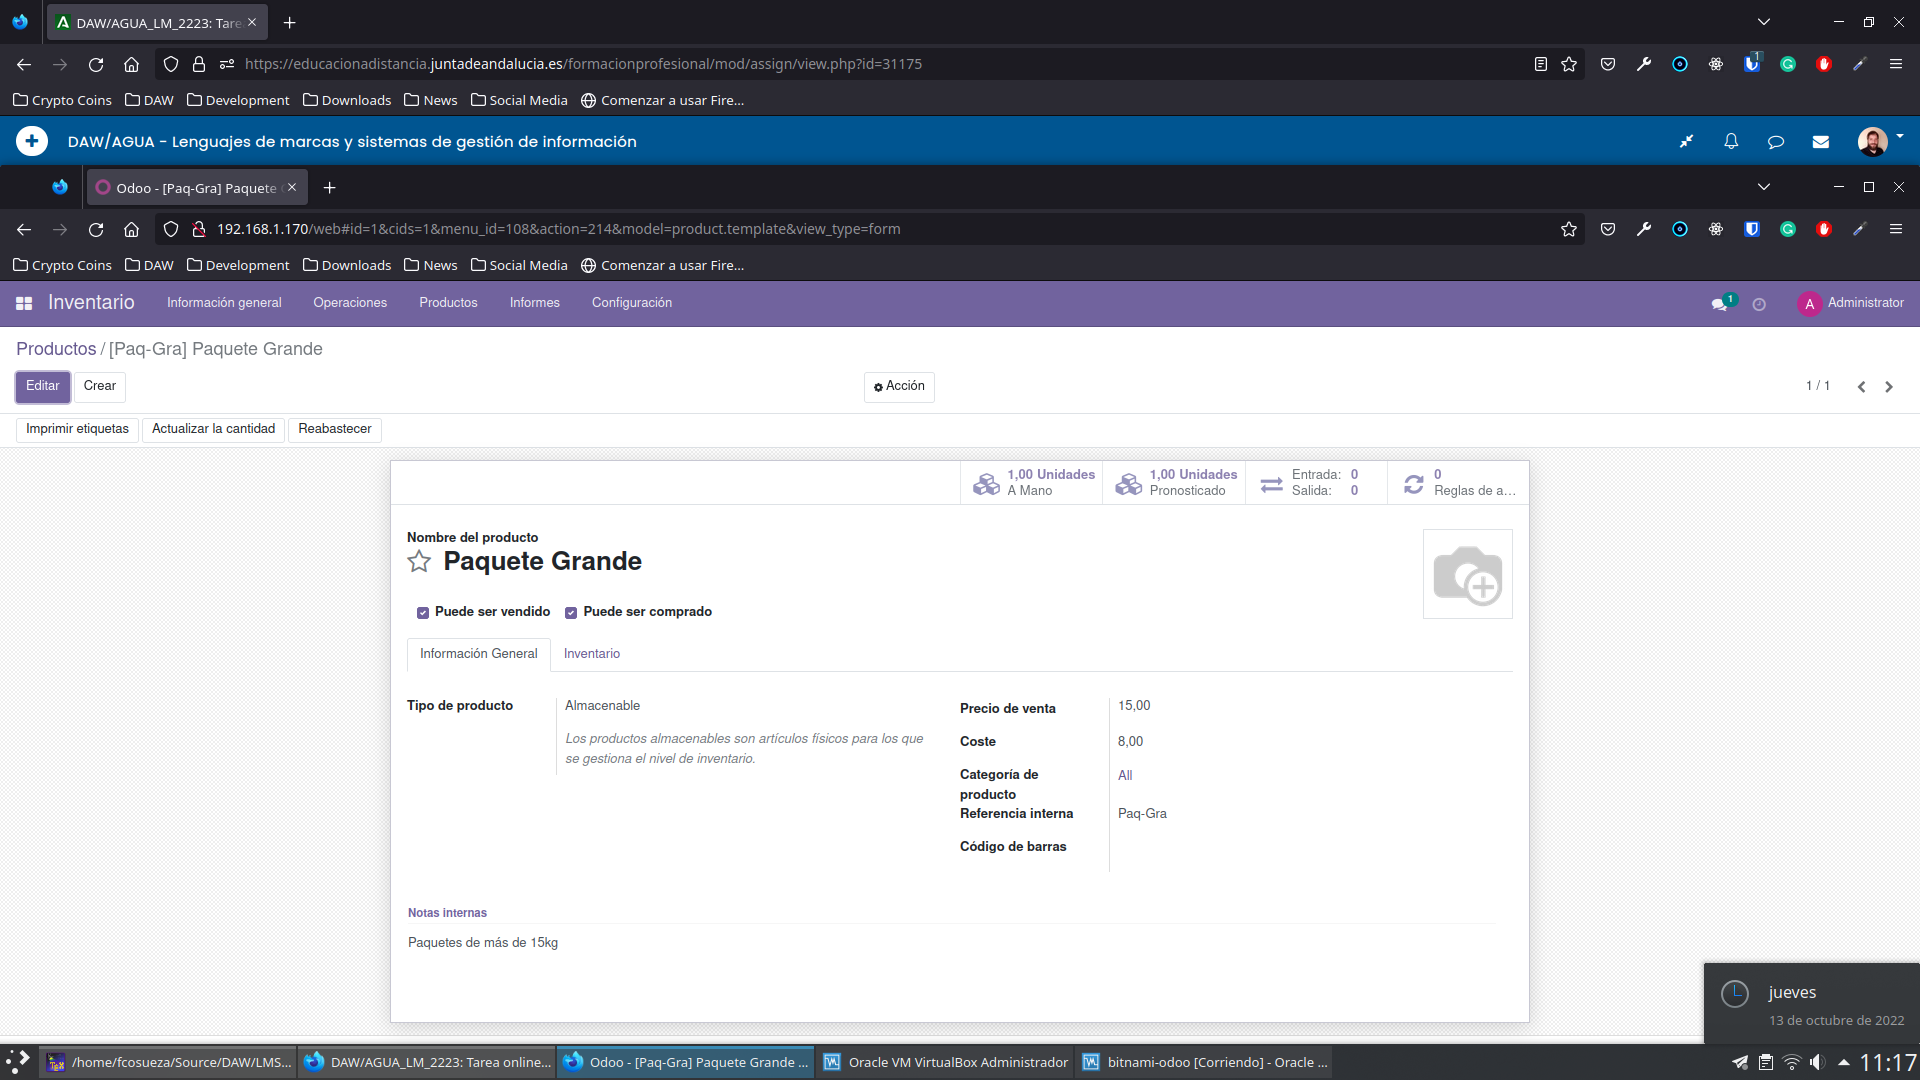
\includegraphics[scale=0.25]{inventario-producto-creado.png}
        \caption{Producto creado}
    \end{figure}
\end{enumerate}

Se han creado tres paquetes diferentes, \textbf{Paquete Grande}, \textbf{Paquete Mediano} y \textbf{Paquete Pequeño}, cada uno con unas características diferentes. En la pagina principal de productos podemos ver todos los paquetes añadidos.

\begin{figure}[ht]
    \centering
    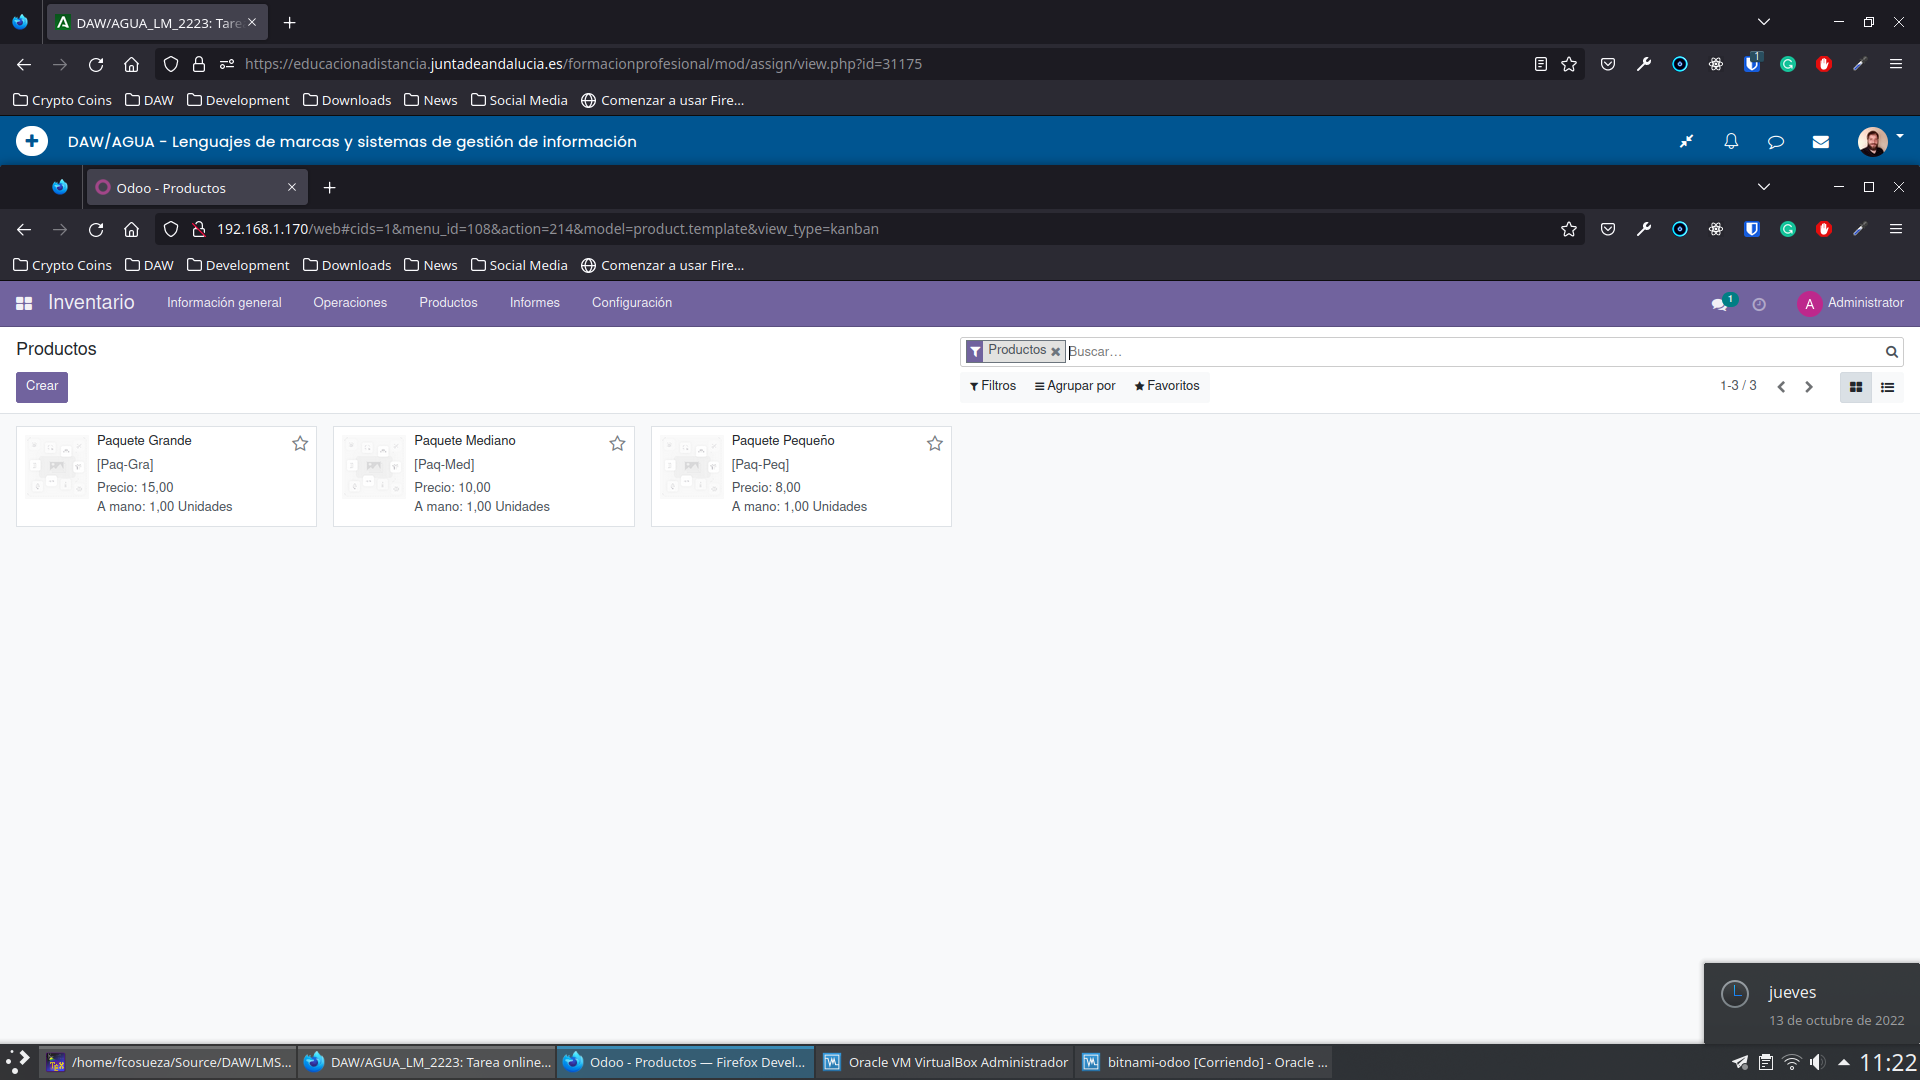
\includegraphics[scale=0.25]{inventario-paquetes-lista.png}
    \caption{Lista de productos creados}
\end{figure}

\vspace{8ex}

\subsection{Generación de Informe de Productos en Stock}
La generación de informes se hace de forma muy sencilla. Para ello solo tendremos que pulsar el \textbf{menu Informes} en la parte superior y seleccionar la opción \textbf{Informe de Inventario}.

Esto nos mostrará una página con la información de todos los productos que tenemos en inventario y en que almacén se encuentran, en nuestro caso en WH/Stock (Warehouse/Stock) que es el que viene por defecto, así como la cantidad de producto,

\begin{figure}[ht]
    \centering
    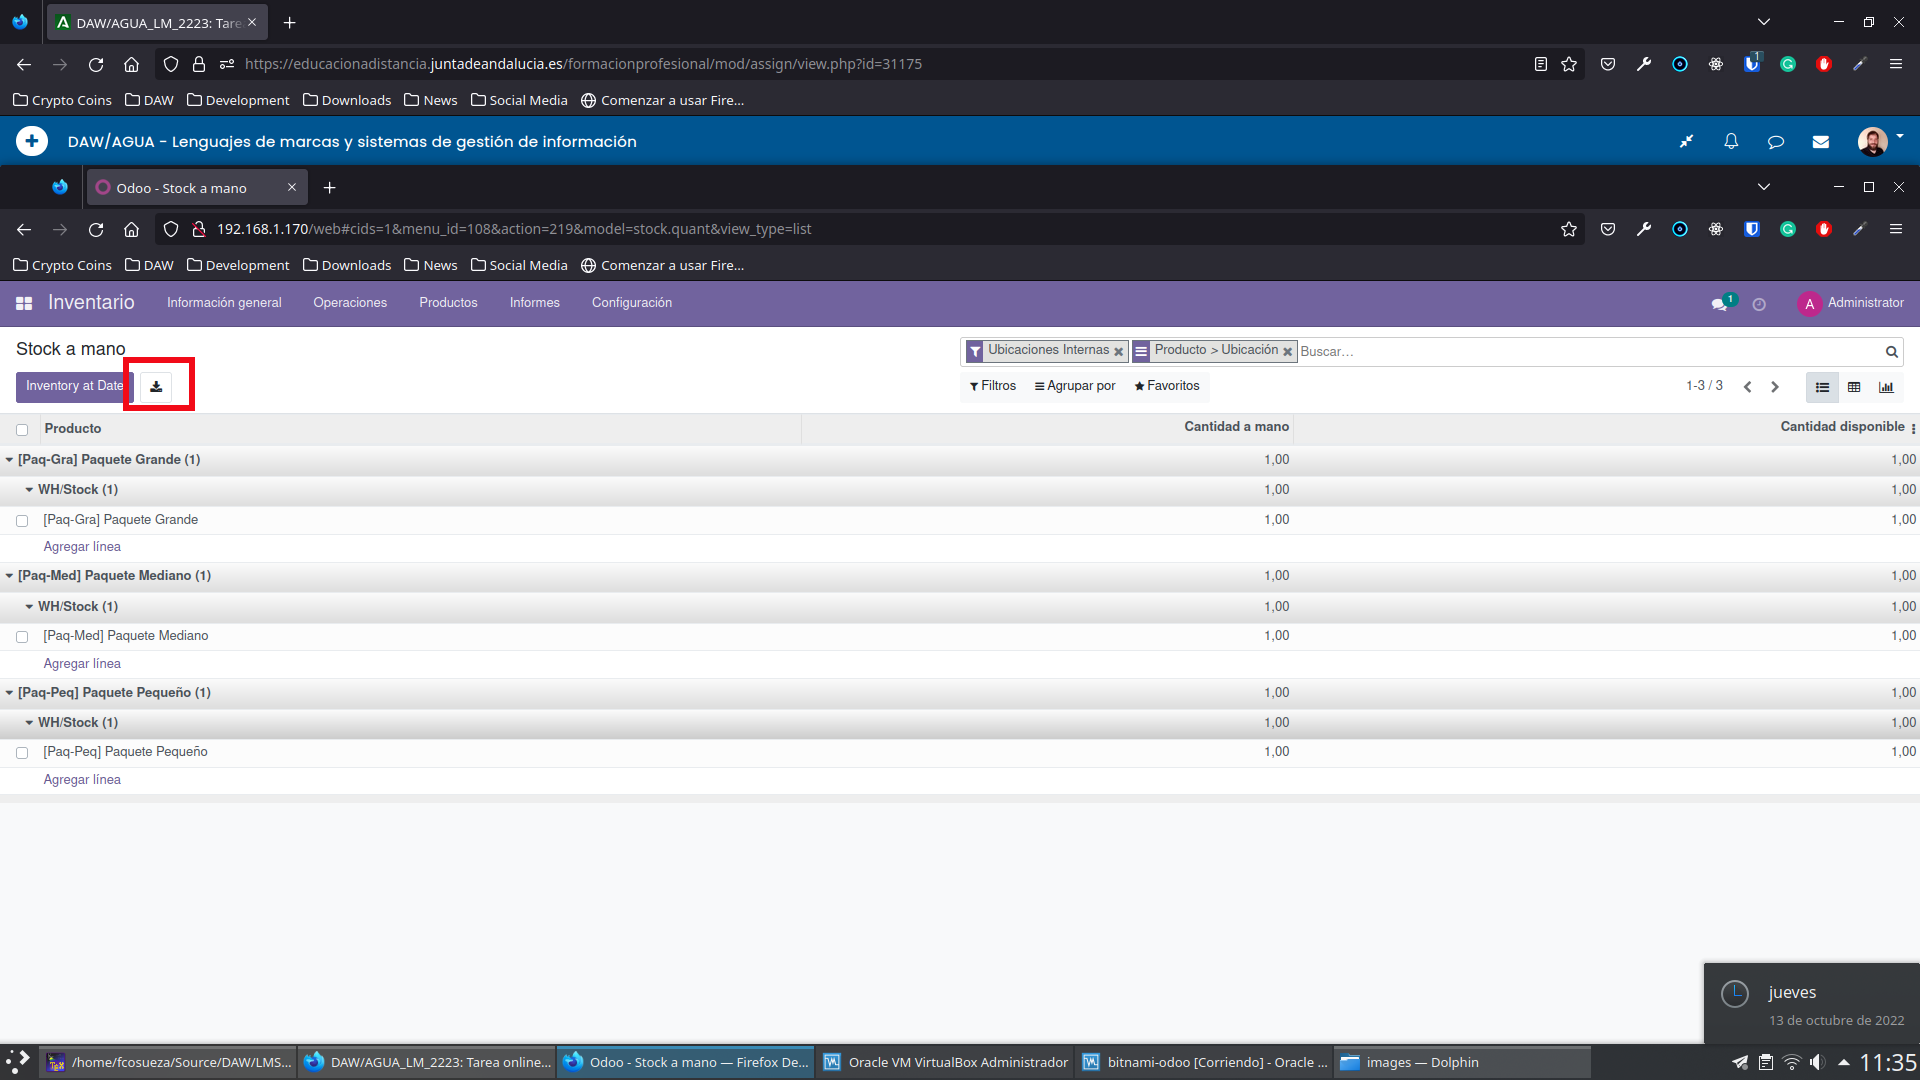
\includegraphics[scale=0.25]{inventario-informe.png}
    \caption{Informe de Inventario}
\end{figure}

Para exportar el informe en formato de \textbf{hoja de cálculo} solo deberemos pulsar el botón \textbf{Exportar todo}, a la derecha de \textbf{Inventory at Date}, remarcado en la captura anterior, y elegir el nombre del fichero en el que queremos almacenarlo y se creará el documento que podremos visualizar con cualquier aplicación de hoja de cálculo. En nuestro caso hemos usado LibreOffice.

\begin{figure}[ht]
    \centering
    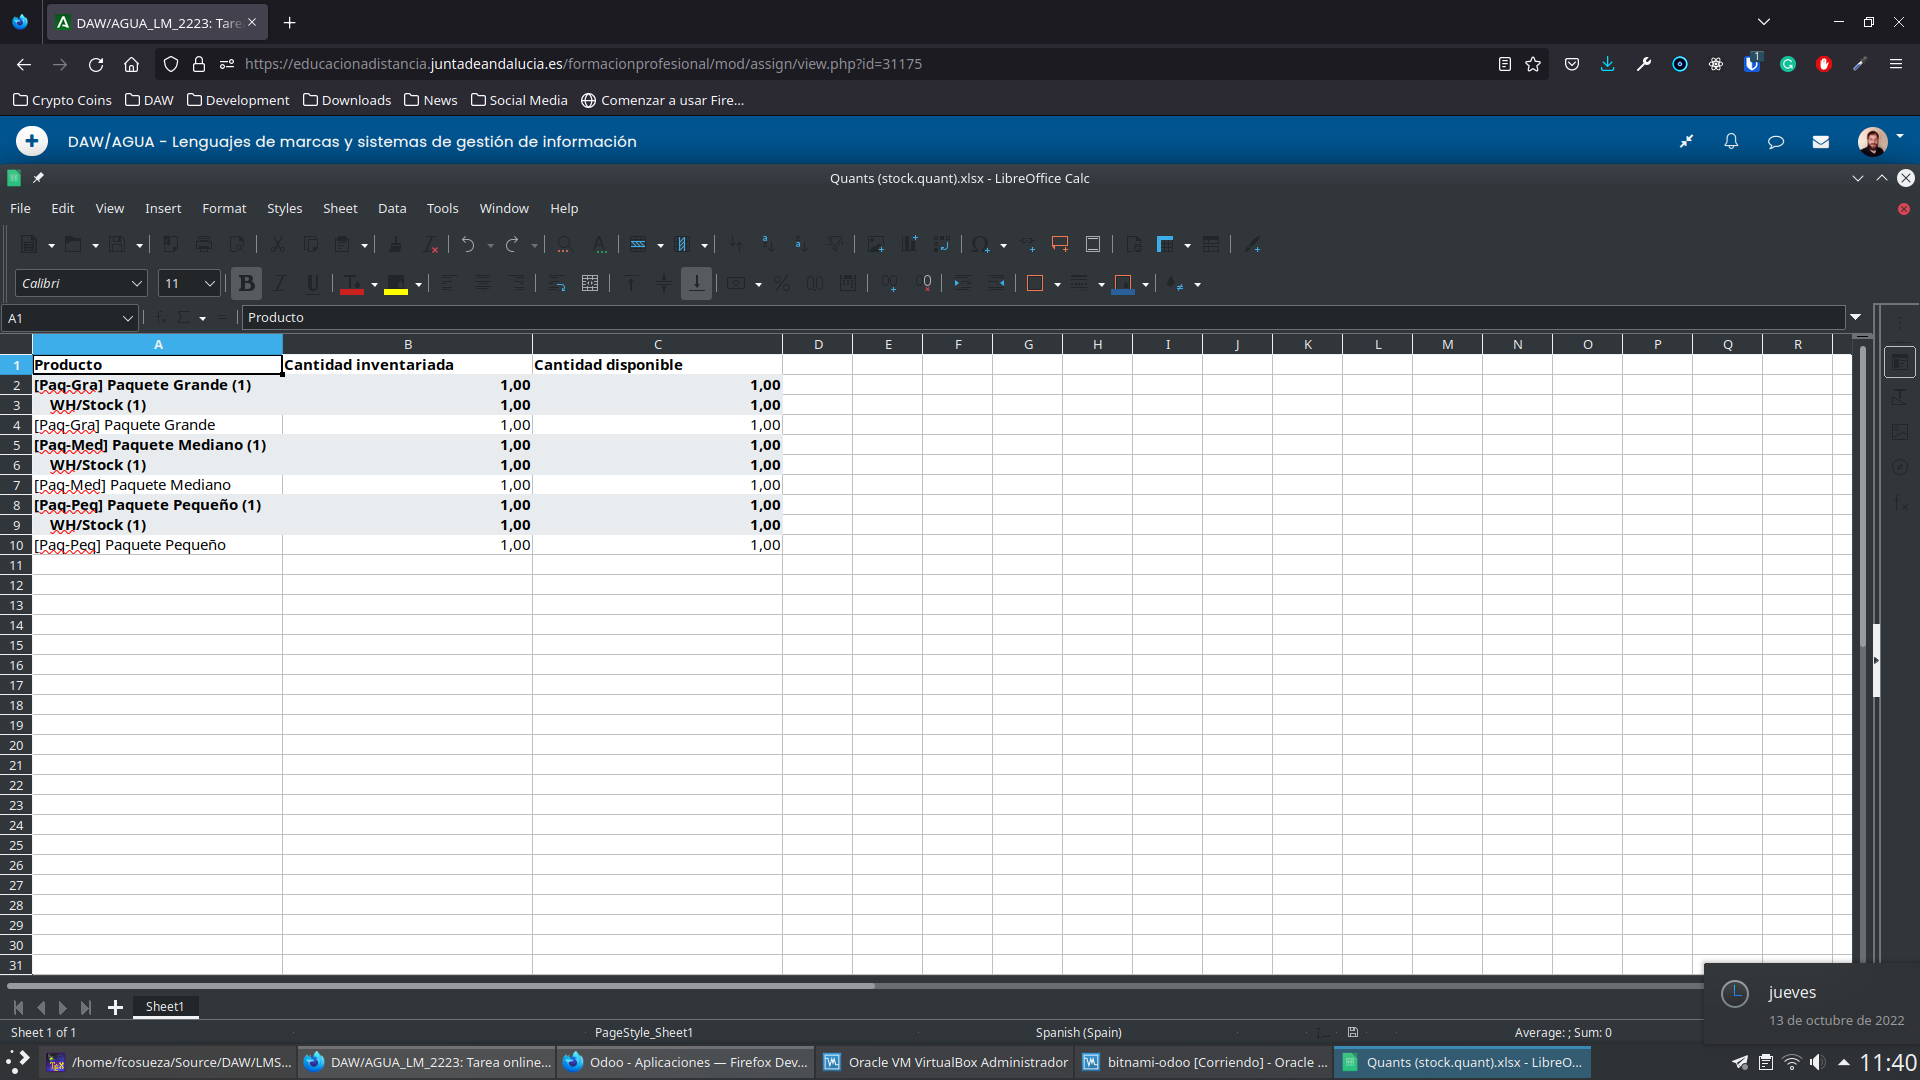
\includegraphics[scale=0.25]{hoja-calculo.png}
    \caption{Informe exportado en una hoja de cálculo}
\end{figure}

\section{Módulo Mantenimiento y Creación de Peticiones}
En este apartado vamos a instalar un módulo nuevo, el \textbf{módulo Mantenimiento}, y vamos a crear dos peticiones de mantenimiento en dos estados diferentes, una \textbf{``En Proceso''} y otra \textbf{``Reparado''}.

La instalación del módulo no se va a cubrir en este apartado ya que es idéntica a la del módulo Inventario que vimos en el apartado anterior, por lo que pasaremos a la \textbf{generación de las peticiones de mantenimiento}.

Para crear una petición de mantenimiento debemos seguir los siguientes pasos:

\begin{enumerate}
    \item En primer lugar, seleccionamos la opción \textbf{Mantenimiento} del menú principal. Eso nos llevará a la pagina principal del módulo donde se mostrarán las peticiones de mantenimiento en curso, en nuestro caso, estará aún vacío. Seleccionamos el menú \textbf{Mantenimiento} y dentro la opción \textbf{Peticiones de mantenimiento}.

    \begin{figure}[ht]
        \centering
        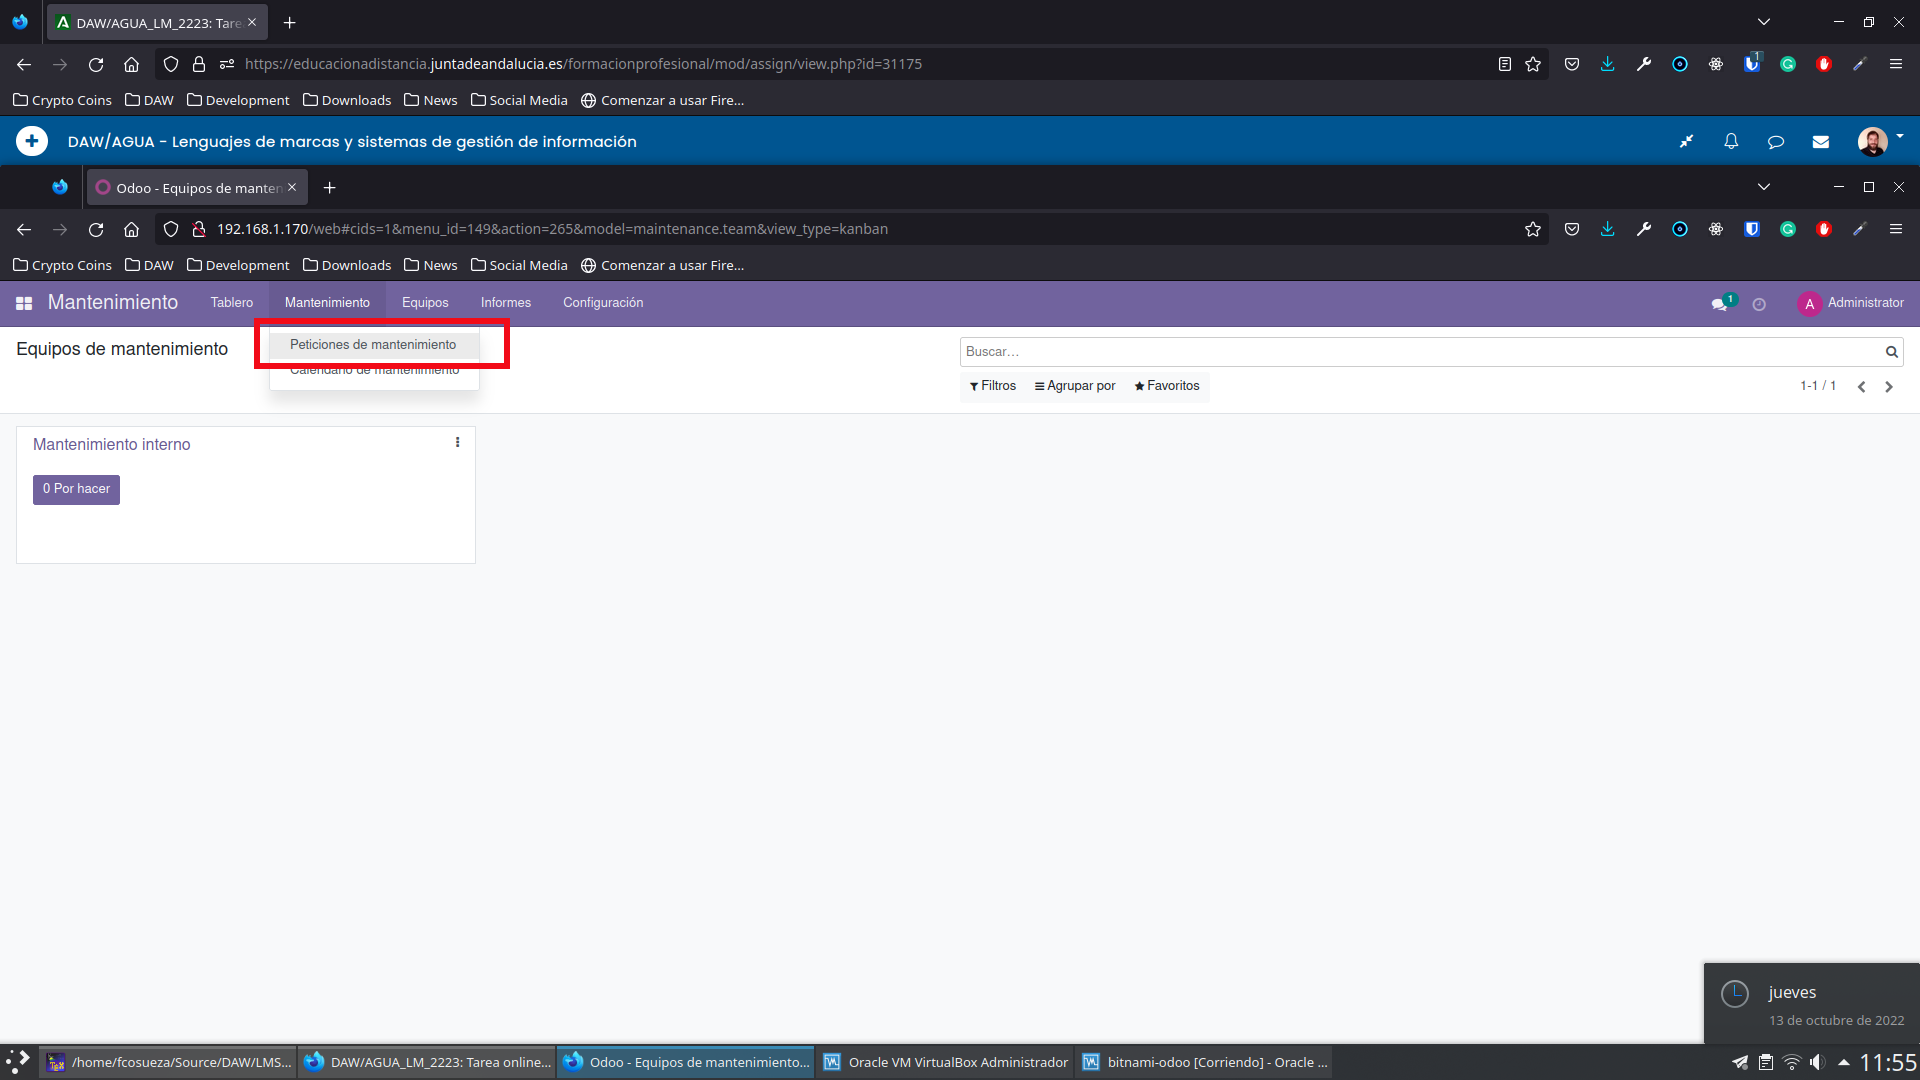
\includegraphics[scale=0.25]{mantenimiento.png}
        \caption{Página principal módulo mantenimiento}
    \end{figure}

    \item Una vez seleccionada la opción, nos llevará a una pagina donde se mostrarán las peticiones actuales y el estado en el que se encuentra. Pulsamos en el botón \textbf{Crear} para iniciar el proceso de creación de la petición.

    \begin{figure}[ht]
        \centering
        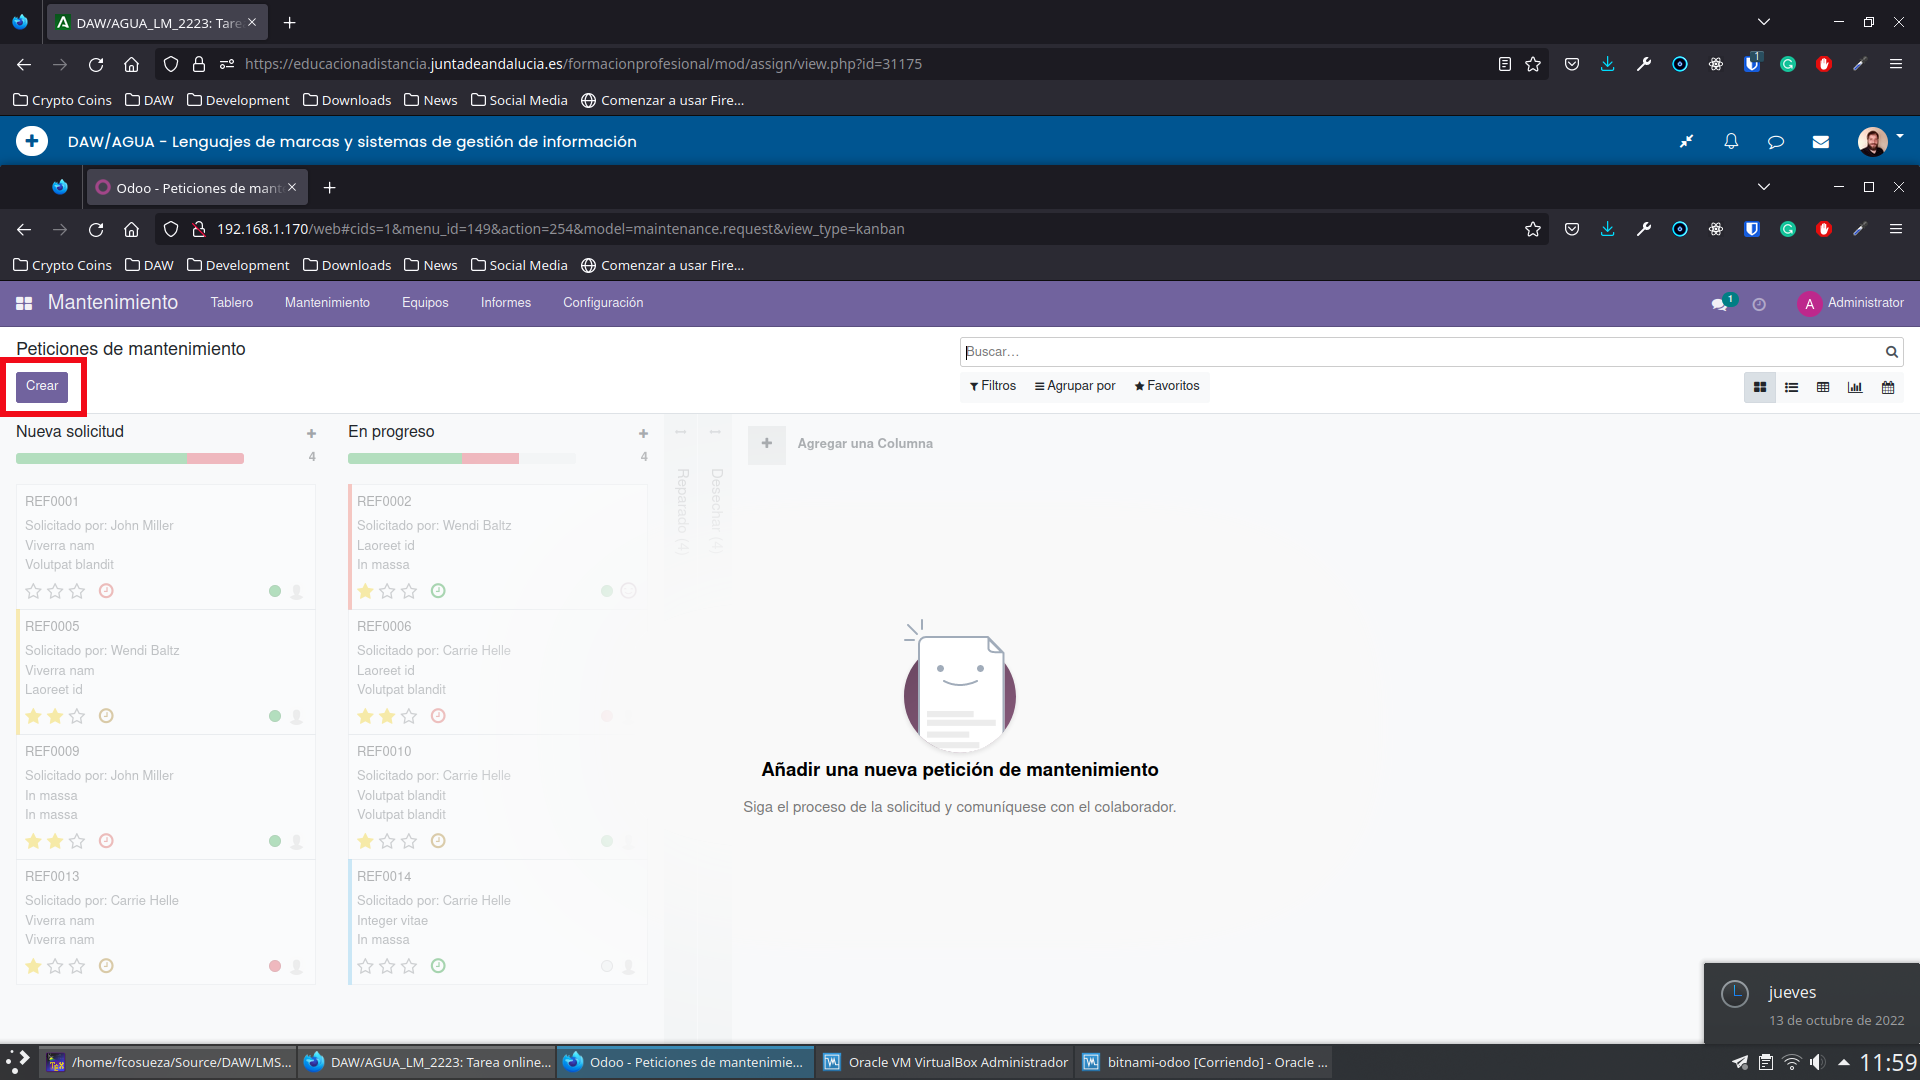
\includegraphics[scale=0.25]{mantenimiento-peticiones.png}
        \caption{Peticiones modulo mantenimiento}
    \end{figure}

    \item En la página de creación de la petición se nos mostrará un formulario con diferentes datos que deberemos introducir, como el \textbf{nombre}, \textbf{fecha de solicitud}, \textbf{tipo de mantenimiento}, \textbf{equipo}, \textbf{responsable}, etc.. Arriba a la izquierda también podemos seleccionar el \textbf{estado} de la petición.

    \begin{figure}[ht]
        \centering
        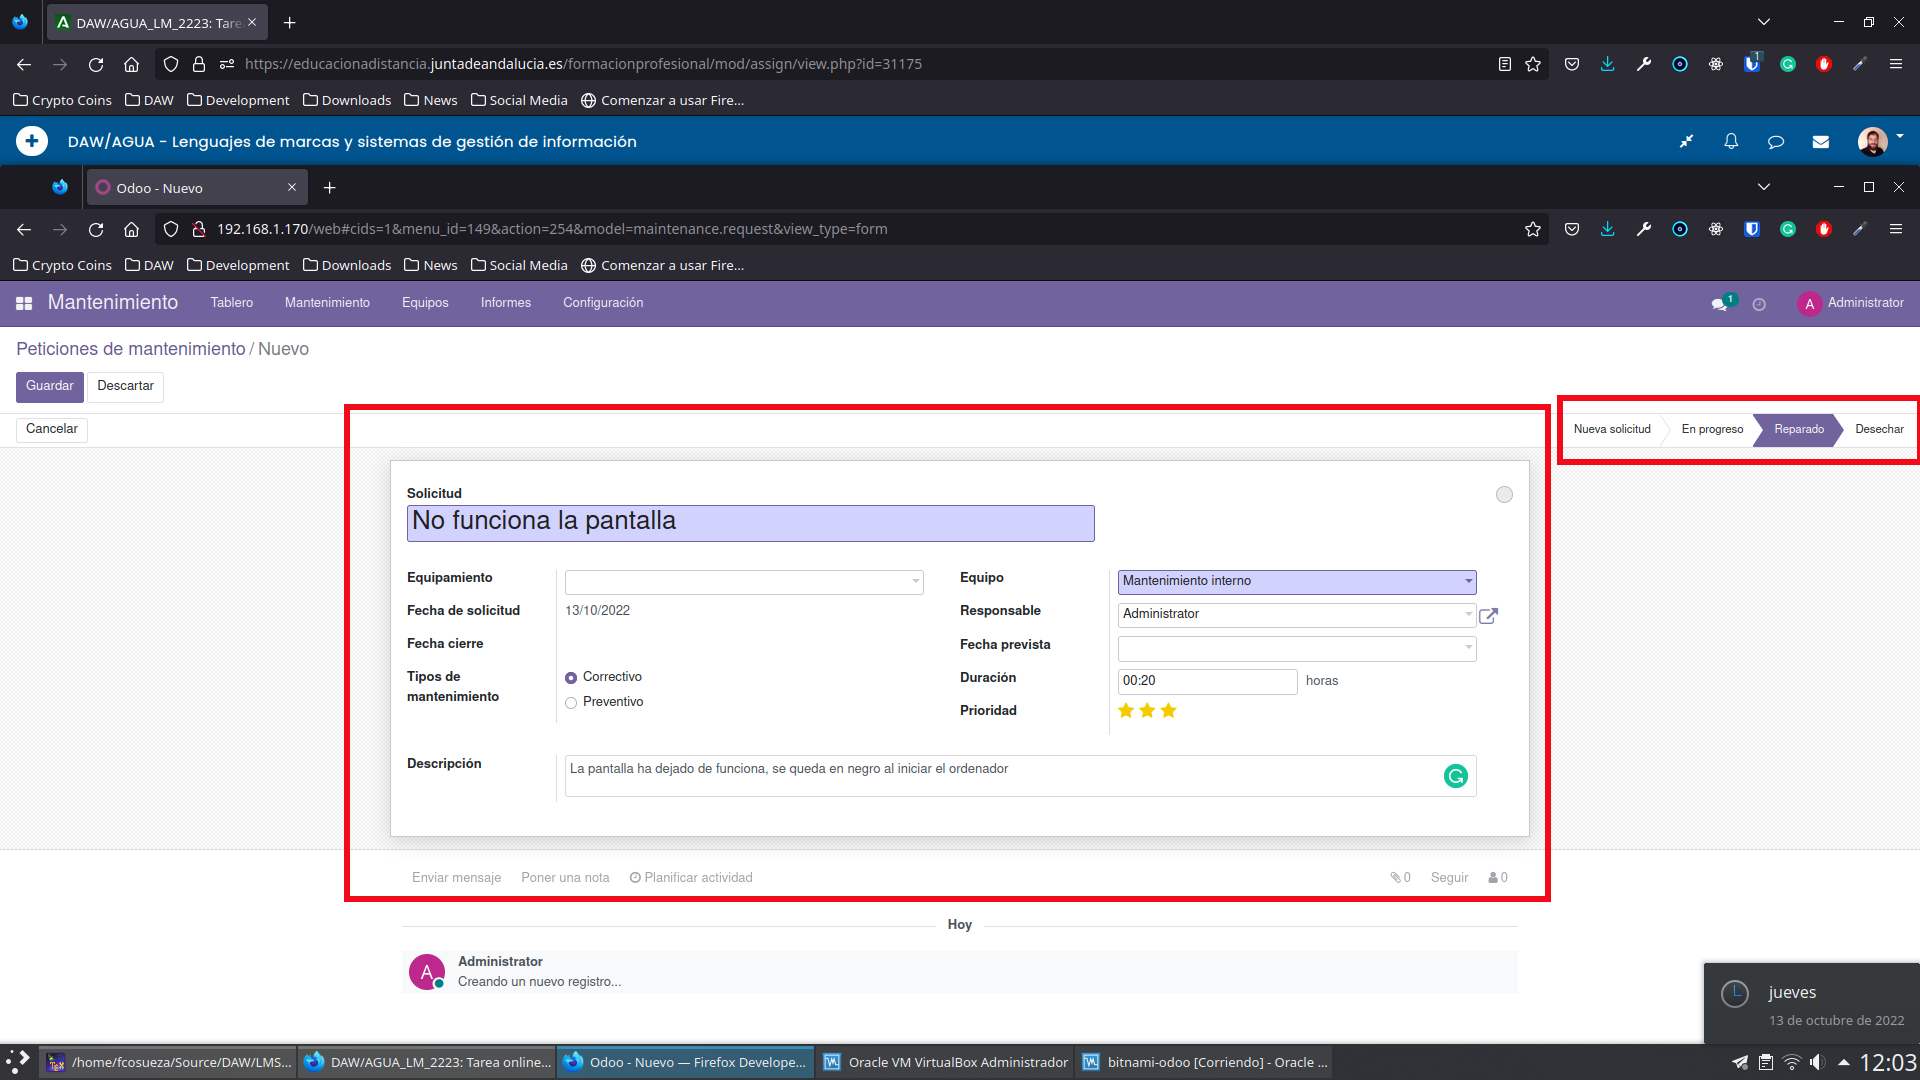
\includegraphics[scale=0.25]{mantenimiento-crear-peticion.png}
        \caption{Creación de petición de mantenimiento}
    \end{figure}

    \item Una vez que hayamos introducido los datos deseados, pulsaremos el botón \textbf{Guardar} y la petición se habrá creado.
\end{enumerate}

Como hemos comentado, se han creado dos peticiones en dos estados diferentes, en la siguiente captura podemos ver las dos peticiones creada y su estado, desde la pantalla principal de peticiones.

\begin{figure}[ht]
    \centering
    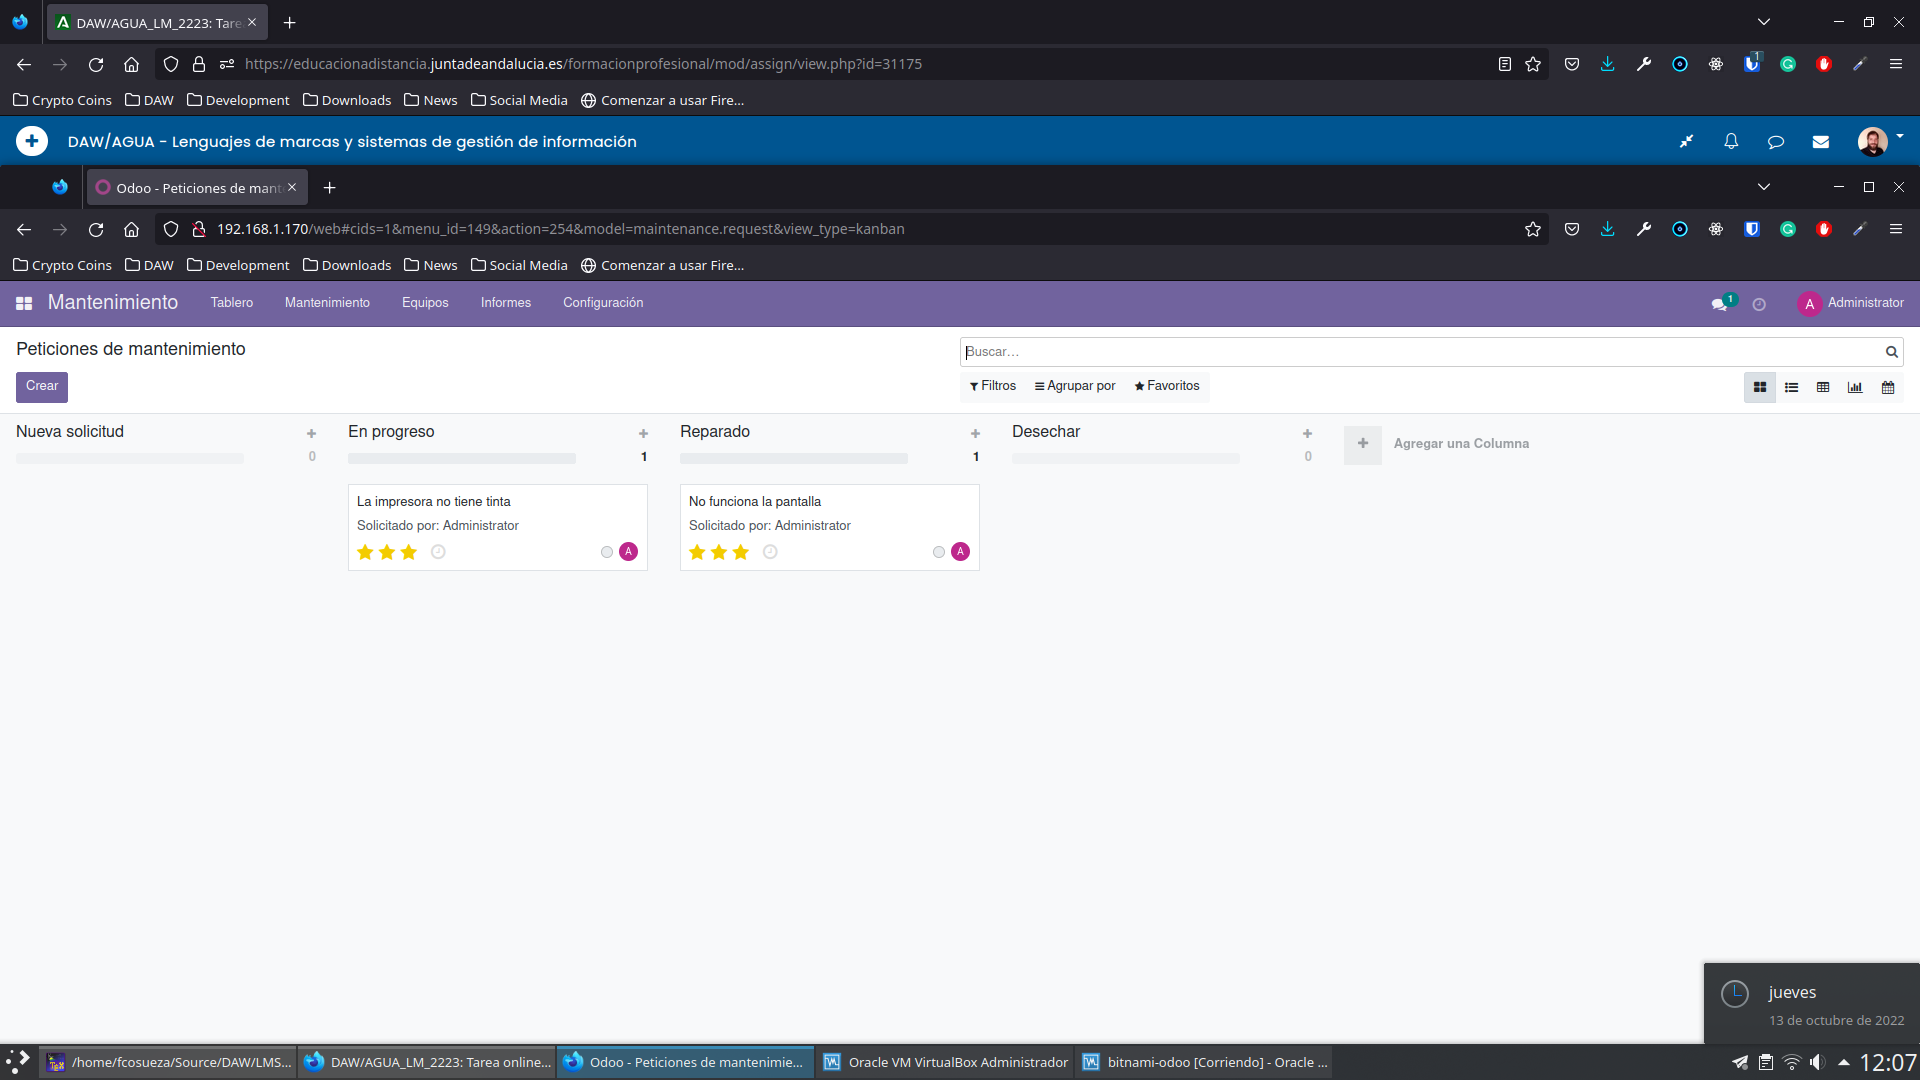
\includegraphics[scale=0.25]{mantenimiento-lista-peticiones.png}
    \caption{Lista de peticiones creadas}
\end{figure}

\vspace{5ex}
Desde esta página podremos mover las tarjetas de las peticiones a la lista que queramos cambiando así su estado, de una forma fácil y rápida, así como \textbf{bloquearlas} o marcarlas como \textbf{listas para la siguiente etapa}

\section{Conclusiones}
Como hemos visto durante este documento \textbf{Odoo} nos ayuda a gestionar todos los aspectos internos de una empresa, siendo una herramienta muy útil a la hora de lidiar con toda la información y procesos que tiene lugar en una compañía.

La instalación y configuración de módulos se lleva a cabo de una forma rápida e intuitiva. Además posee una extensa documentación, así como ayuda en línea proporcionada por Odoobot y que hace que el proceso de aprendizaje sea mucho más rápido y ameno.

Cabe destacar que Odoo tiene dos versiones, siendo la gratuita la que nosotros hemos usado en este documento. La versión de pago añade mas funcionalidad y actualizaciones para los diferentes módulos que componen la aplicación.
% Bibliography

%\newpage
%\bibliography{citas}
%\bibliographystyle{unsrt}

\end{document}